%%%%%%%%%%%%%%%%%%%%%%%%%%%%%%%%%%%%%%%%%%%%%%%%%%%%%%%%%%%%
%%% LaPreprint: PREPRINT TEMPLATE
%%%%%%%%%%%%%%%%%%%%%%%%%%%%%%%%%%%%%%%%%%%%%%%%%%%%%%%%%%%%


%%%%%%%%%%%%%%%%%%%%%%%%%%%%%%%%%%%%%%%%%%%%%%%%%%%%%%%%%%%%
%%% PREAMBLE
%%%%%%%%%%%%%%%%%%%%%%%%%%%%%%%%%%%%%%%%%%%%%%%%%%%%%%%%%%%%

% Declare document class
\documentclass[9pt]{lapreprint}
% Choose between "biorxiv", "medrxiv", "arxiv" and "chemrxiv". Otherwise defaults "Preprint".
% Choose between "blue" and "red" colour scheme. Defaults to "blue".
% Use the "onehalfspacing" option for 1.5 line spacing.
% Use the "doublespacing" option for 2.0 line spacing.
% Use the "lineno" option for line numbers.
% Use the "endfloat" option to place floats (images etc) after the bibliography.

% Import packages
\usepackage{lipsum}     % Required to insert dummy text
%\usepackage[version=4]{mhchem} % For chemical notation
\usepackage{siunitx}    % For SI units
\usepackage{pdflscape}  % For putting pages in landscape mode
%\usepackage{rotating}   % For rotating specific elements
\usepackage{textgreek}  % Greek symbols
\usepackage{gensymb}    % Symbols
\usepackage[misc]{ifsym} % For the \Letter symbol
\usepackage{orcidlink}  % For the \orcidlink
\usepackage{listings}   % For inserting code chunks
\usepackage{colortbl}   % For Knitr table colouring
\usepackage{tabularx}   % For making Knitr tables compatible
\usepackage{longtable}  % For multi-page tables
\usepackage{caption}
\usepackage{subcaption}
\usepackage{subscript}
\usepackage{multirow}
\usepackage{snotez}     % For sidenote environments. enotez for endnotes
\usepackage{csquotes}   % For language-based quote rules (helps BiBLaTeX)
\usepackage{textcomp}
\usepackage{todonotes}
\usepackage{booktabs}
%\usepackage{unicode-math}
\usepackage{siunitx}
\usepackage{longtable} % for 'longtable' environment

\usepackage{pifont}
\usepackage{placeins}
\DeclareRobustCommand{\textbigstar}{\mbox{\ding{72}}}

% for supplement
\renewcommand{\thetable}{S\arabic{table}}

% Make declarations
\DeclareSIUnit\Molar{M}

% Please note that these options may affect formatting. 

%%%%%%%%%%%%%%%%%%%%%%%%%%%%%%%%%%%%%%%%%%%%%%%%%%%%%%%%%%%%
%%% BIBLIOGRAPHYan
%%%%%%%%%%%%%%%%%%%%%%%%%%%%%%%%%%%%%%%%%%%%%%%%%%%%%%%%%%%%
\usepackage[			% use biblatex for bibliography
	backend=biber,      % use biber or bibtex backend
    style=numeric, %authoryear,   % choose style
	natbib=true,		% allow natbib commands
	hyperref=true,	    % activate hyperref support
	alldates=year,      % only show year (not month)
]{biblatex}

% Update to your bibliography file
\addbibresource{src/TOAM.bib}

%%%%%%%%%%%%%%%%%%%%%%%%%%%%%%%%%%%%%%%%%%%%%%%%%%%%%%%%%%%%
%%% ARTICLE SETUP
%%%%%%%%%%%%%%%%%%%%%%%%%%%%%%%%%%%%%%%%%%%%%%%%%%%%%%%%%%%%

% Paper title
%\title{Silent Memories: \\ Trajectory of memory traces}
%\title{Forgotten memories can be reactivated and influence behaviour outside of conscious access}
%\title{Forgotten memories can be reactivated and influence behaviour unconsciously}

%TC:ignore
\title{}
\title{
  Supplemental Information \\
  \vspace{1em}
  \large Neural Traces of Forgotten Memories Persist in Humans and are Behaviorally Relevant}


% Authors - you can use \orcidlink{} and \authfn{} - see contribution note

\author[]{Tom Willems, Konstantinos Zervas, Finn Rabe, Andrea Federspiel, Katharina Henke}


% Affiliations
%\affil[1]{Institute of Psychology, University of Bern}
%\affil[2]{Support Center for Advanced Neuroimaging, Translational Imaging Center (sitem-insel), Institute for Diagnostic and Interventional Neuroradiology, Inselspital – University of Bern}
% Other metadata. Feel free to add your own
\metadata[]{\Letter\hspace{.5ex} For correspondence}{\url{https://github.com/TomW92/TOAM/issues}}
%\metadata[\authfn{1}\authfn{2}\authfn{3}]{}{Here's a few symbols to denote contribution specifics, e.g. authors who contributed equally to the work.}
\metadata[]{Present address}{Cognitive Neuroscience of Memory and Consciousness, Institute of Psychology, University of Bern, Fabrikstrasse 8, 3012, Bern}
\metadata[]{Data availability}{Code available via GitHub, see above, preprocessed data is available via the UniBern Server, external access can be granted by the corresponding author.}%, otherwise see \href{https://zenodo.org/}{Zenodo}.}
\metadata[]{Funding}{This research was supported by SNSF Advanced Grant TMAG-1\_209374 to K. Henke and by the University of Bern Sitem-Insel-Support Grant to K. Henke.}
\metadata[]{Competing interests}{The authors declare no competing interests.}


% Surname of the lead author(s) for the running footer
\leadauthor{}
\shorttitle{}

%%%%%%%%%%%%%%%%%%%%%%%%%%%%%%%%%%%%%%%%%%%%%%%%%%%%%%%%%%%%
%%% ARTICLE START
%%%%%%%%%%%%%%%%%%%%%%%%%%%%%%%%%%%%%%%%%%%%%%%%%%%%%%%%%%%%

\begin{document}
\maketitle
\fussy

\newpage
\section{Supplementary Figures}
 \begin{figure}[!ht]
    \centering
     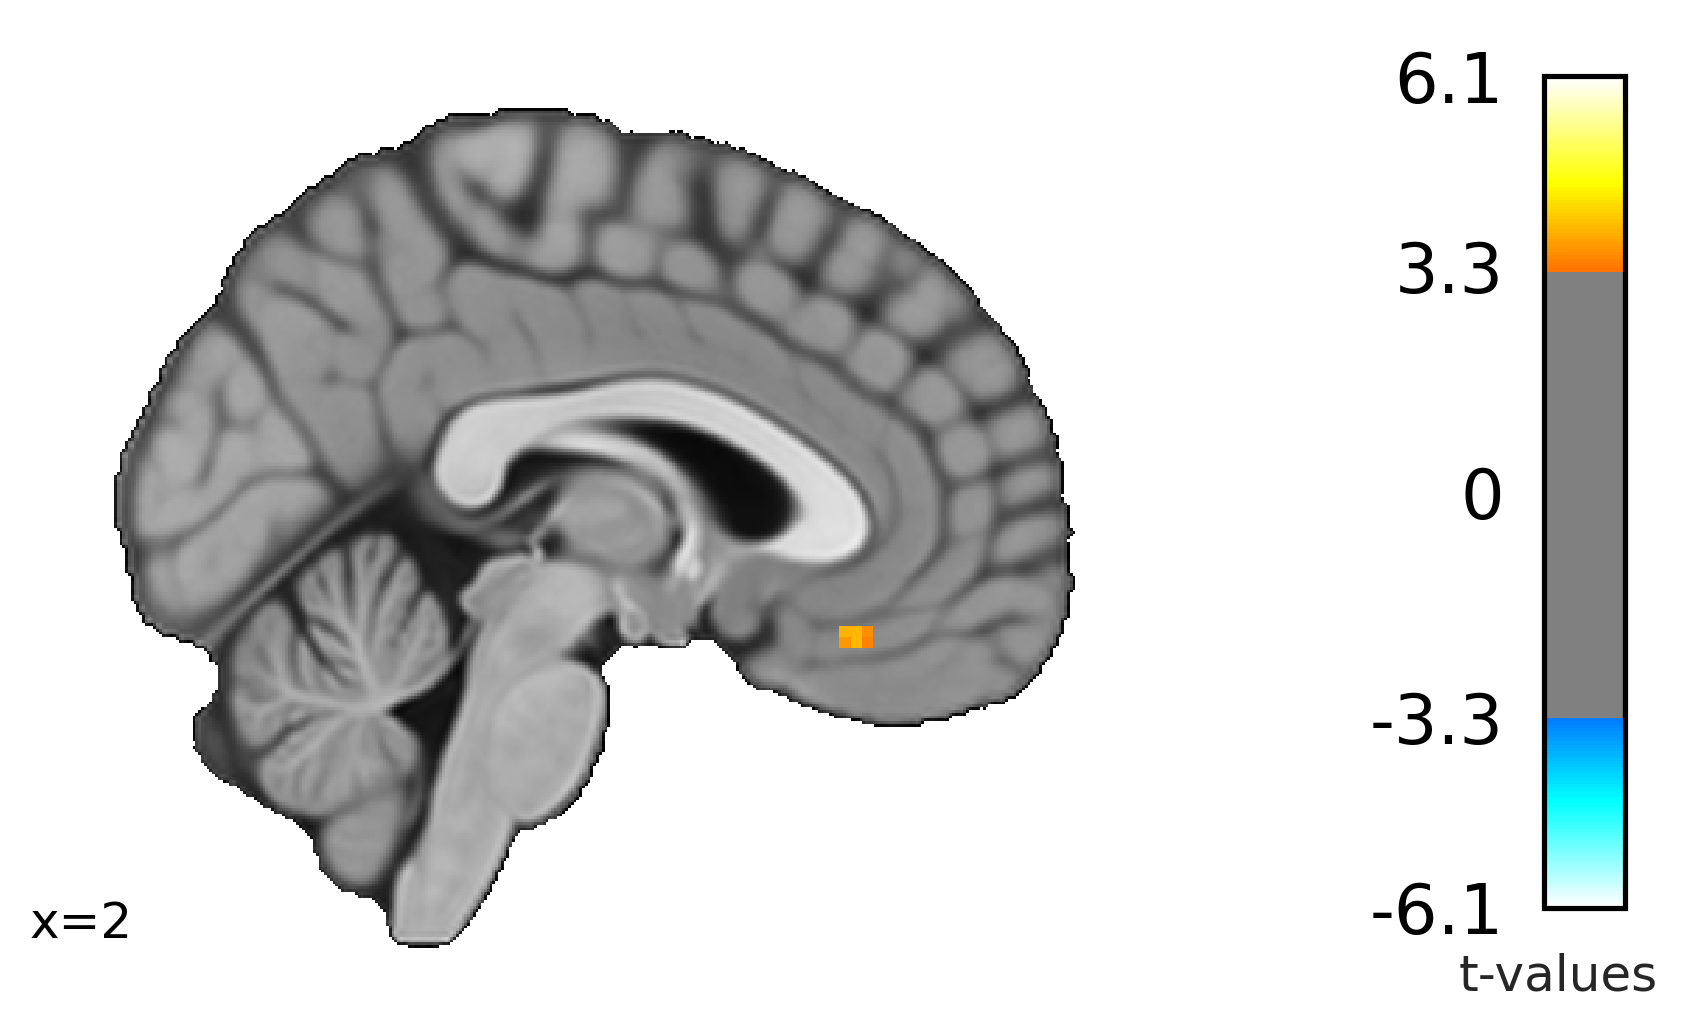
\includegraphics[width=\linewidth/2]{paper/src/figures/FigureS1_inaccessible_subsequent.png}
     \caption*{\textbf{Figure S1. Medial prefrontal cortex activation during guess responses given at the 24-hour category retrieval predicted the subsequent regain of conscious access to the memories.} \\ \vspace{0.5em}
     Medial prefrontal component of the episodic retrieval network predicted conscious recognition success. We contrasted the guess responses on the 24-hour category retrieval task that would subsequently yield correct sure responses on the recognition task with those other guess responses given on the 24-hour category task that would subsequently yield correct guess responses on the recognition task. This revealed a cluster in the medial prefrontal cortex (peak at MNI [0, 30, -16], p\textsubscript{uncor} < 0.001, T(18) = 4.19). Results presented in this panel were acquired with the whole-brain fMRI sequence. See Table S12 for details.}
\end{figure}

\newpage


 \begin{figure}[!ht]
    \centering
\begin{subfigure}[]{0.6\linewidth}
    \centering
    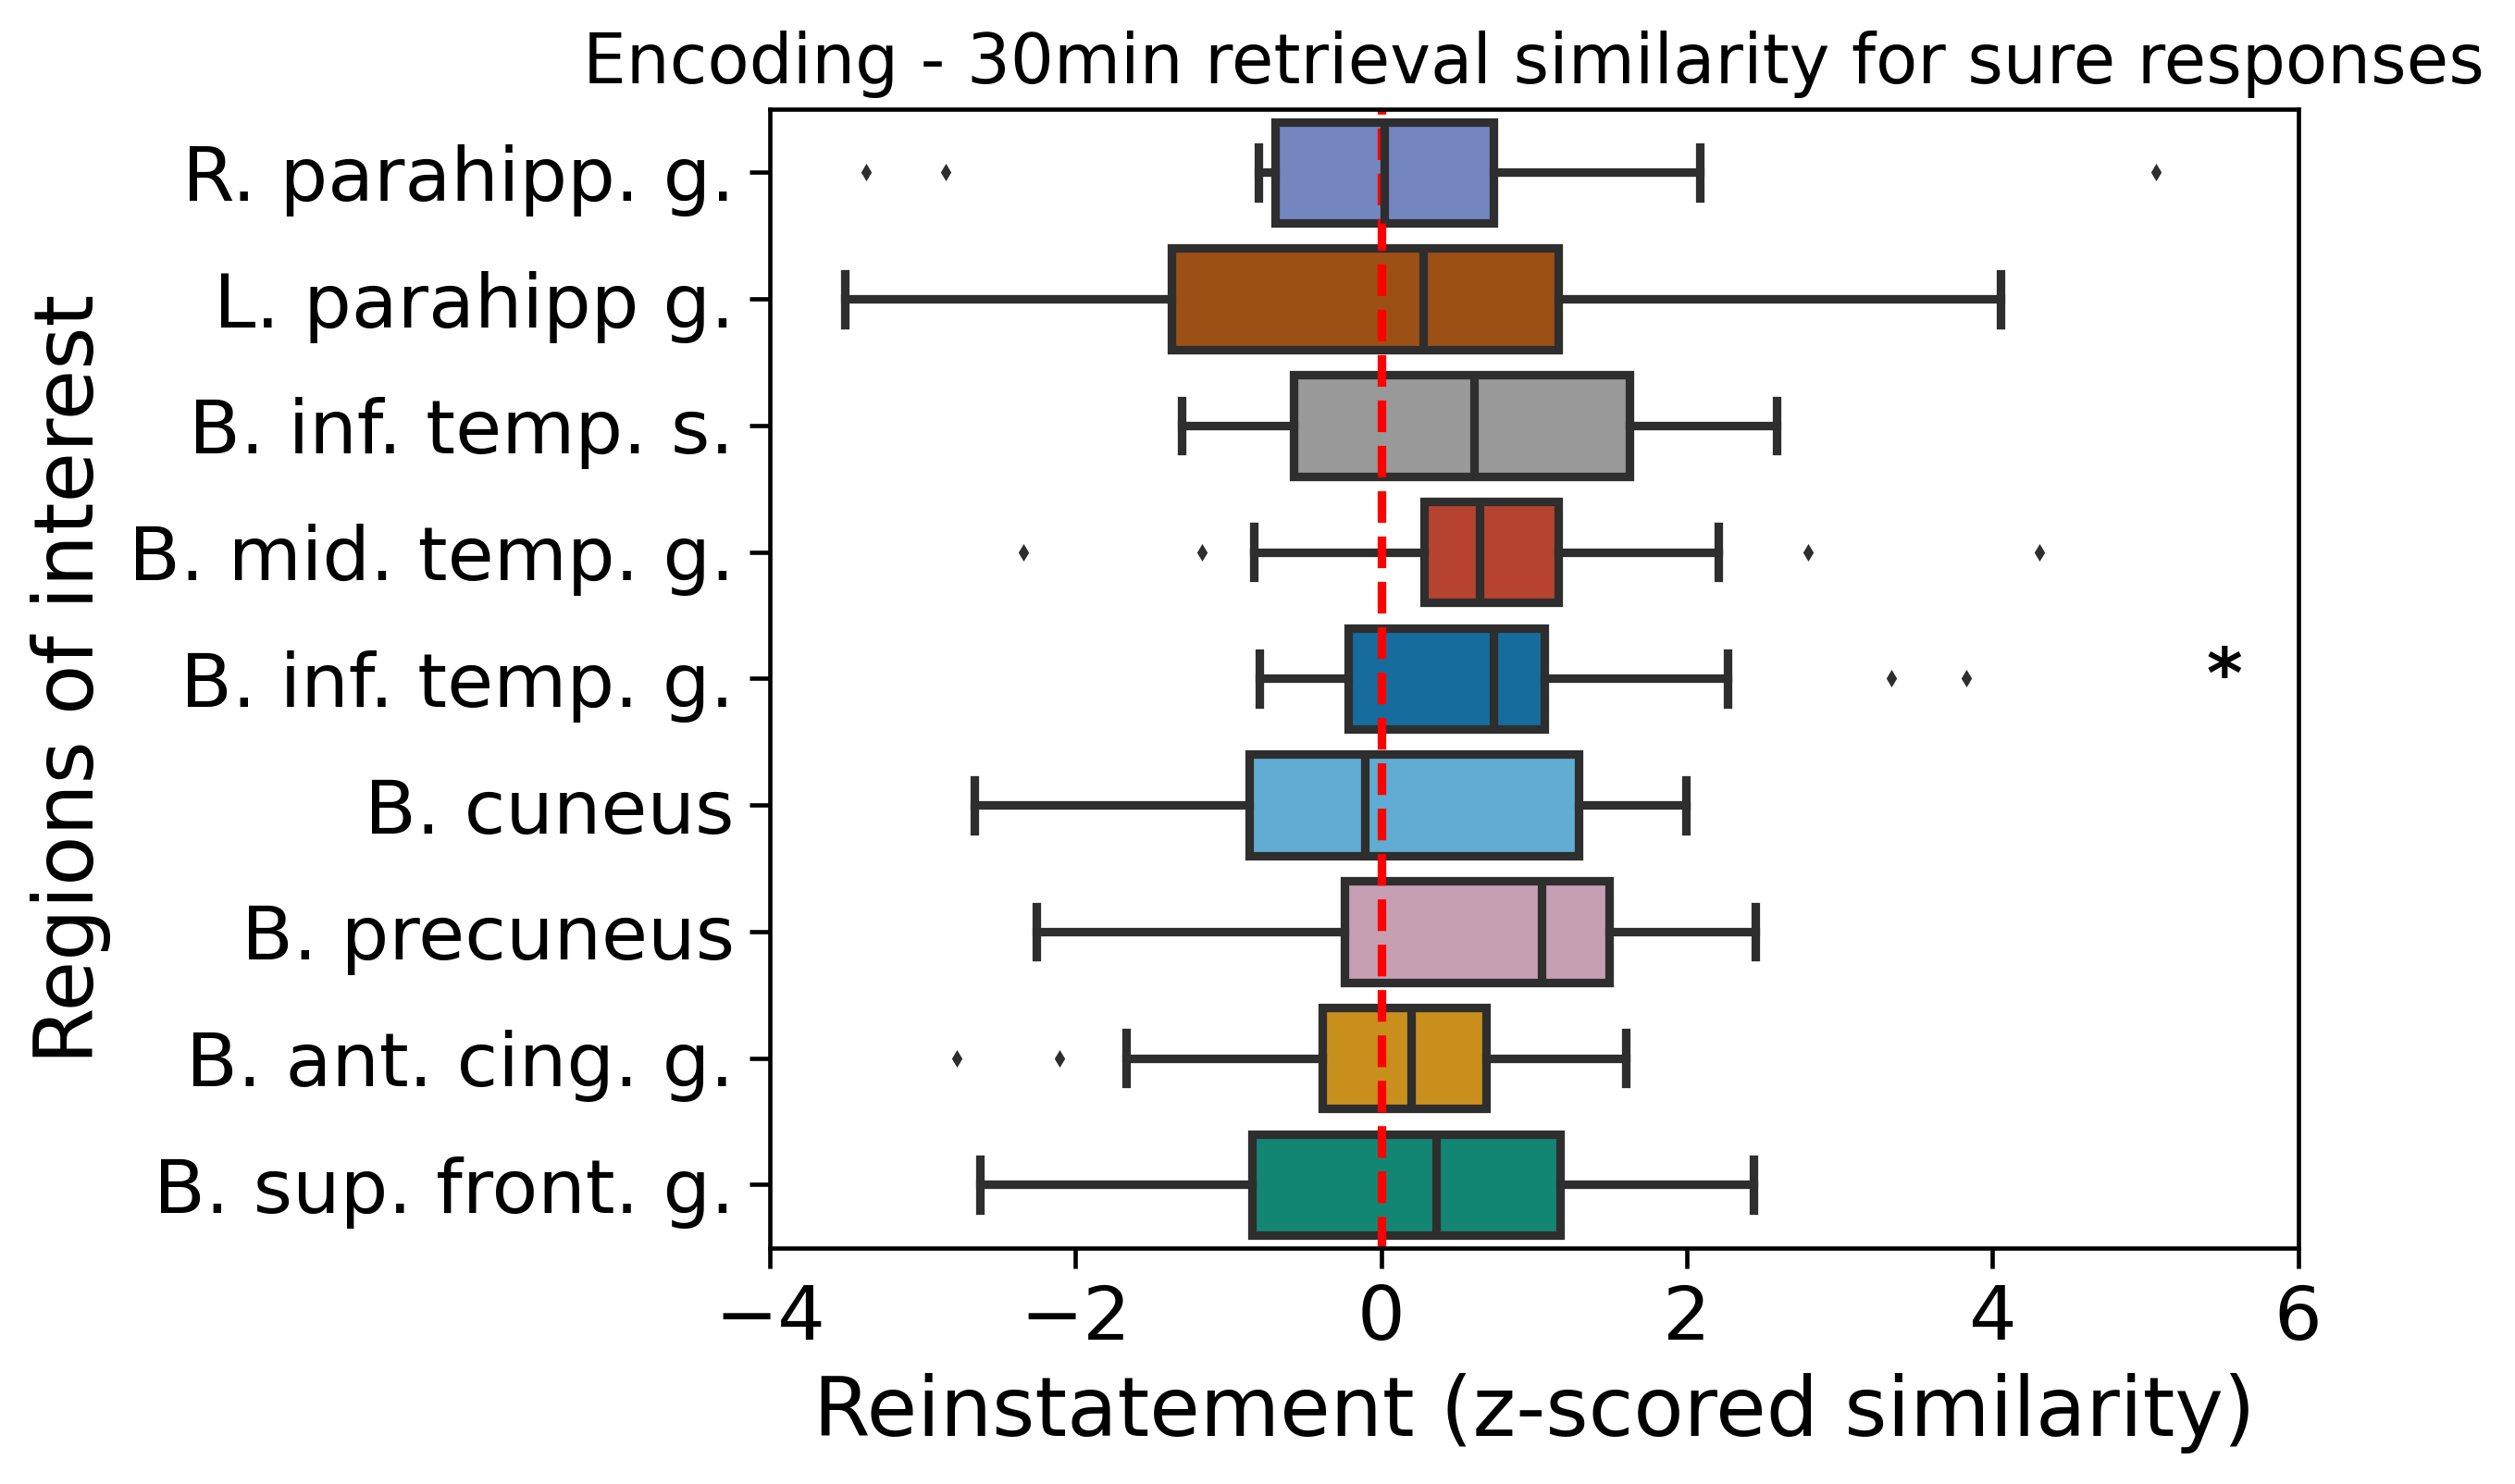
\includegraphics[width=\linewidth]{paper/src/figures/20240530_wb-array_n__enc_ret1_perm_consc_consc-unconsc_incorr.png}
\end{subfigure}
\begin{subfigure}[]{0.19\linewidth}
    \centering
    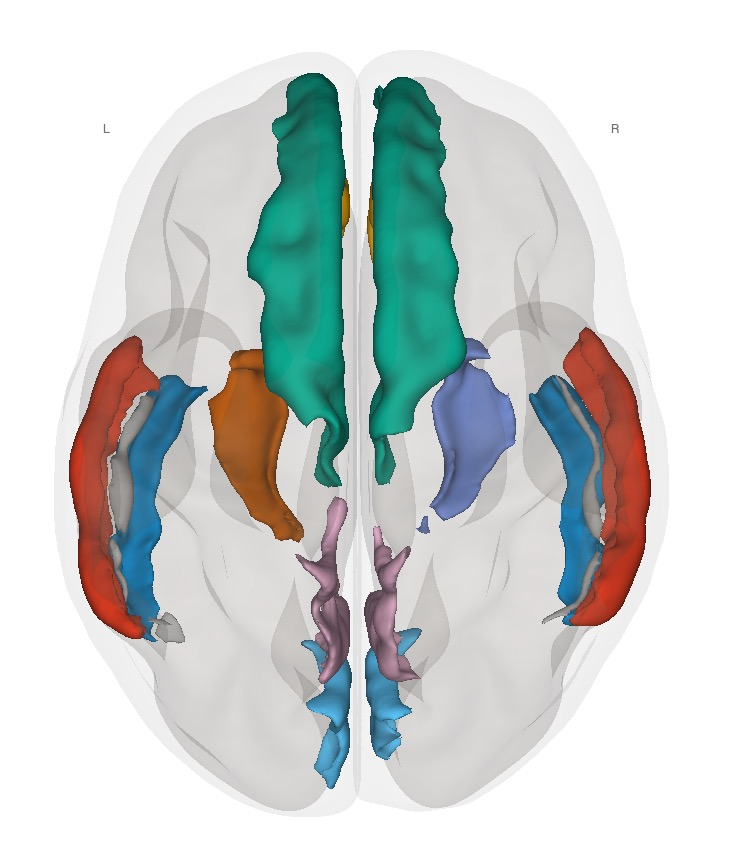
\includegraphics[width=\linewidth]{paper/src/figures/wb_rois_top.jpg}
\end{subfigure}
\begin{subfigure}[]{0.19\linewidth}
    \centering
    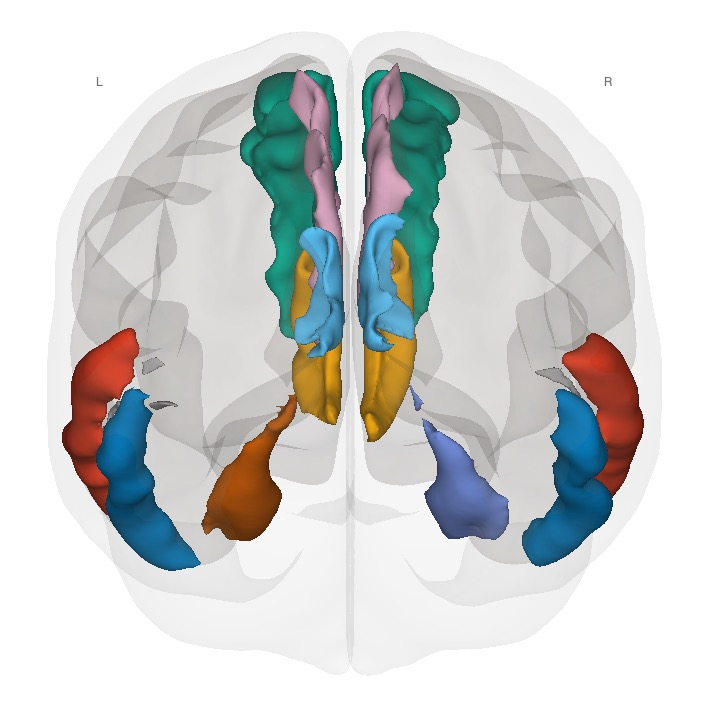
\includegraphics[width=\linewidth]{paper/src/figures/wb_rois_back.jpg}
\end{subfigure}
     \caption*{\textbf{Figure S2. Similarity of voxel patterns between encoding and the 30-minute category retrieval task were relevant for retrieval accuracy.} \\ \vspace{0.5em}
Encoding – retrieval similarity (ERS) analysis for the 30-minute category retrieval yielded significance in the bilateral inferior temporal gyrus for correct sure responses (t(16) = 2.3, p = 0.035, B\textsubscript{10} = 1.9).  Results presented in this panel were acquired with the whole-brain fMRI sequence. *p < 0.05, **p < 0.01 by Student’s t test. Abbreviations: R., right; L., left; B., bilateral; parahipp., parahippocampus; inf., inferior; mid., middle; ant., anterior; cing., cingulate; sup., superior; front., frontal; s., sulcus, g., gyrus.
}
\end{figure}

\newpage


 \begin{figure}[!ht]
    \centering
     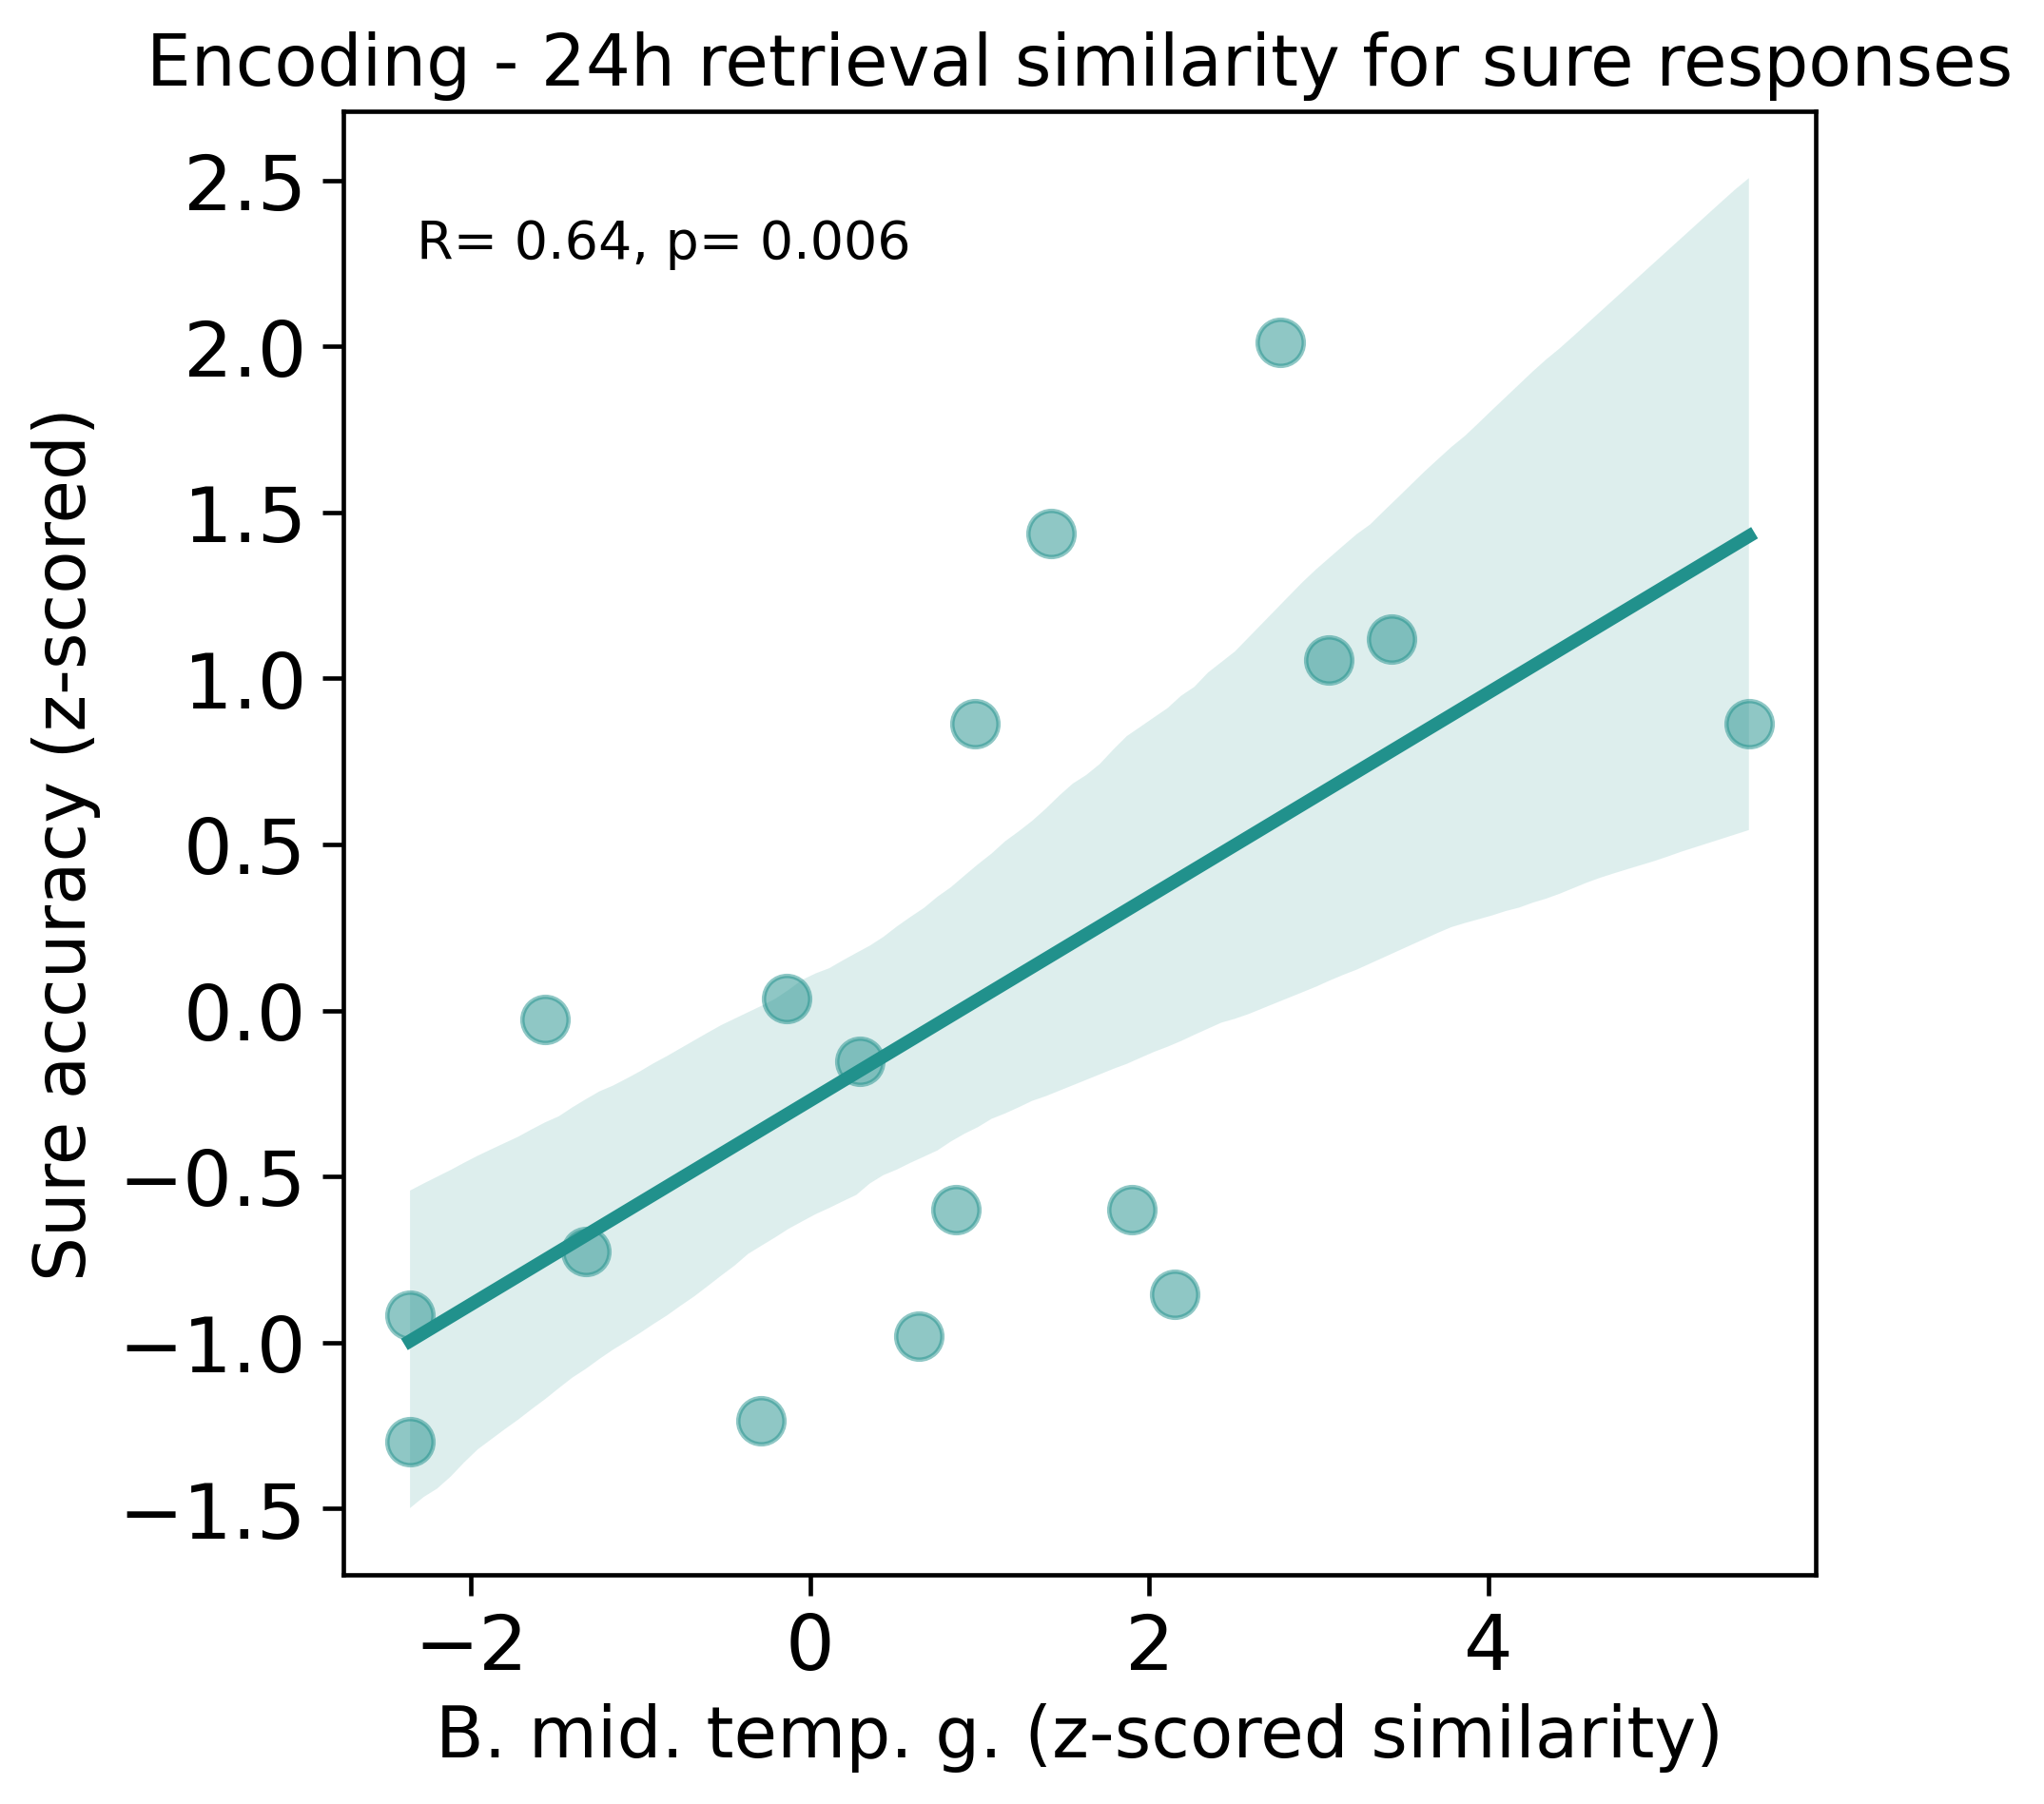
\includegraphics[width=0.6\linewidth]{paper/src/figures/20240530_wb-array_n__enc_ret2_perm_consc_consc-unconsc_incorr_B. mid. temp. g._ERS_correl.png}
     \caption*{\textbf{Figure S3. Similarity of voxel patterns between encoding and the 24-hour category retrieval were relevant for retrieval success.} \\ \vspace{0.5em}
   Encoding - 24-hour category retrieval similarity in bilateral middle temporal gyrus underlying correct sure responses given on the category retrieval task revealed a non-significant mean value comparison but a significant between-subjects correlation with the accuracy of sure responses given on the 24-hour category task (number of correct sure trials, p = 0.006, R = 0.64, B\textsubscript{10} = 10.4). Results presented in this panel were acquired with the whole-brain fMRI sequence. Abbreviations: B., bilateral; mid., middle; temp., temporal; g., gyrus.}
\end{figure}

\newpage

 \begin{figure}[!ht]
    \centering
     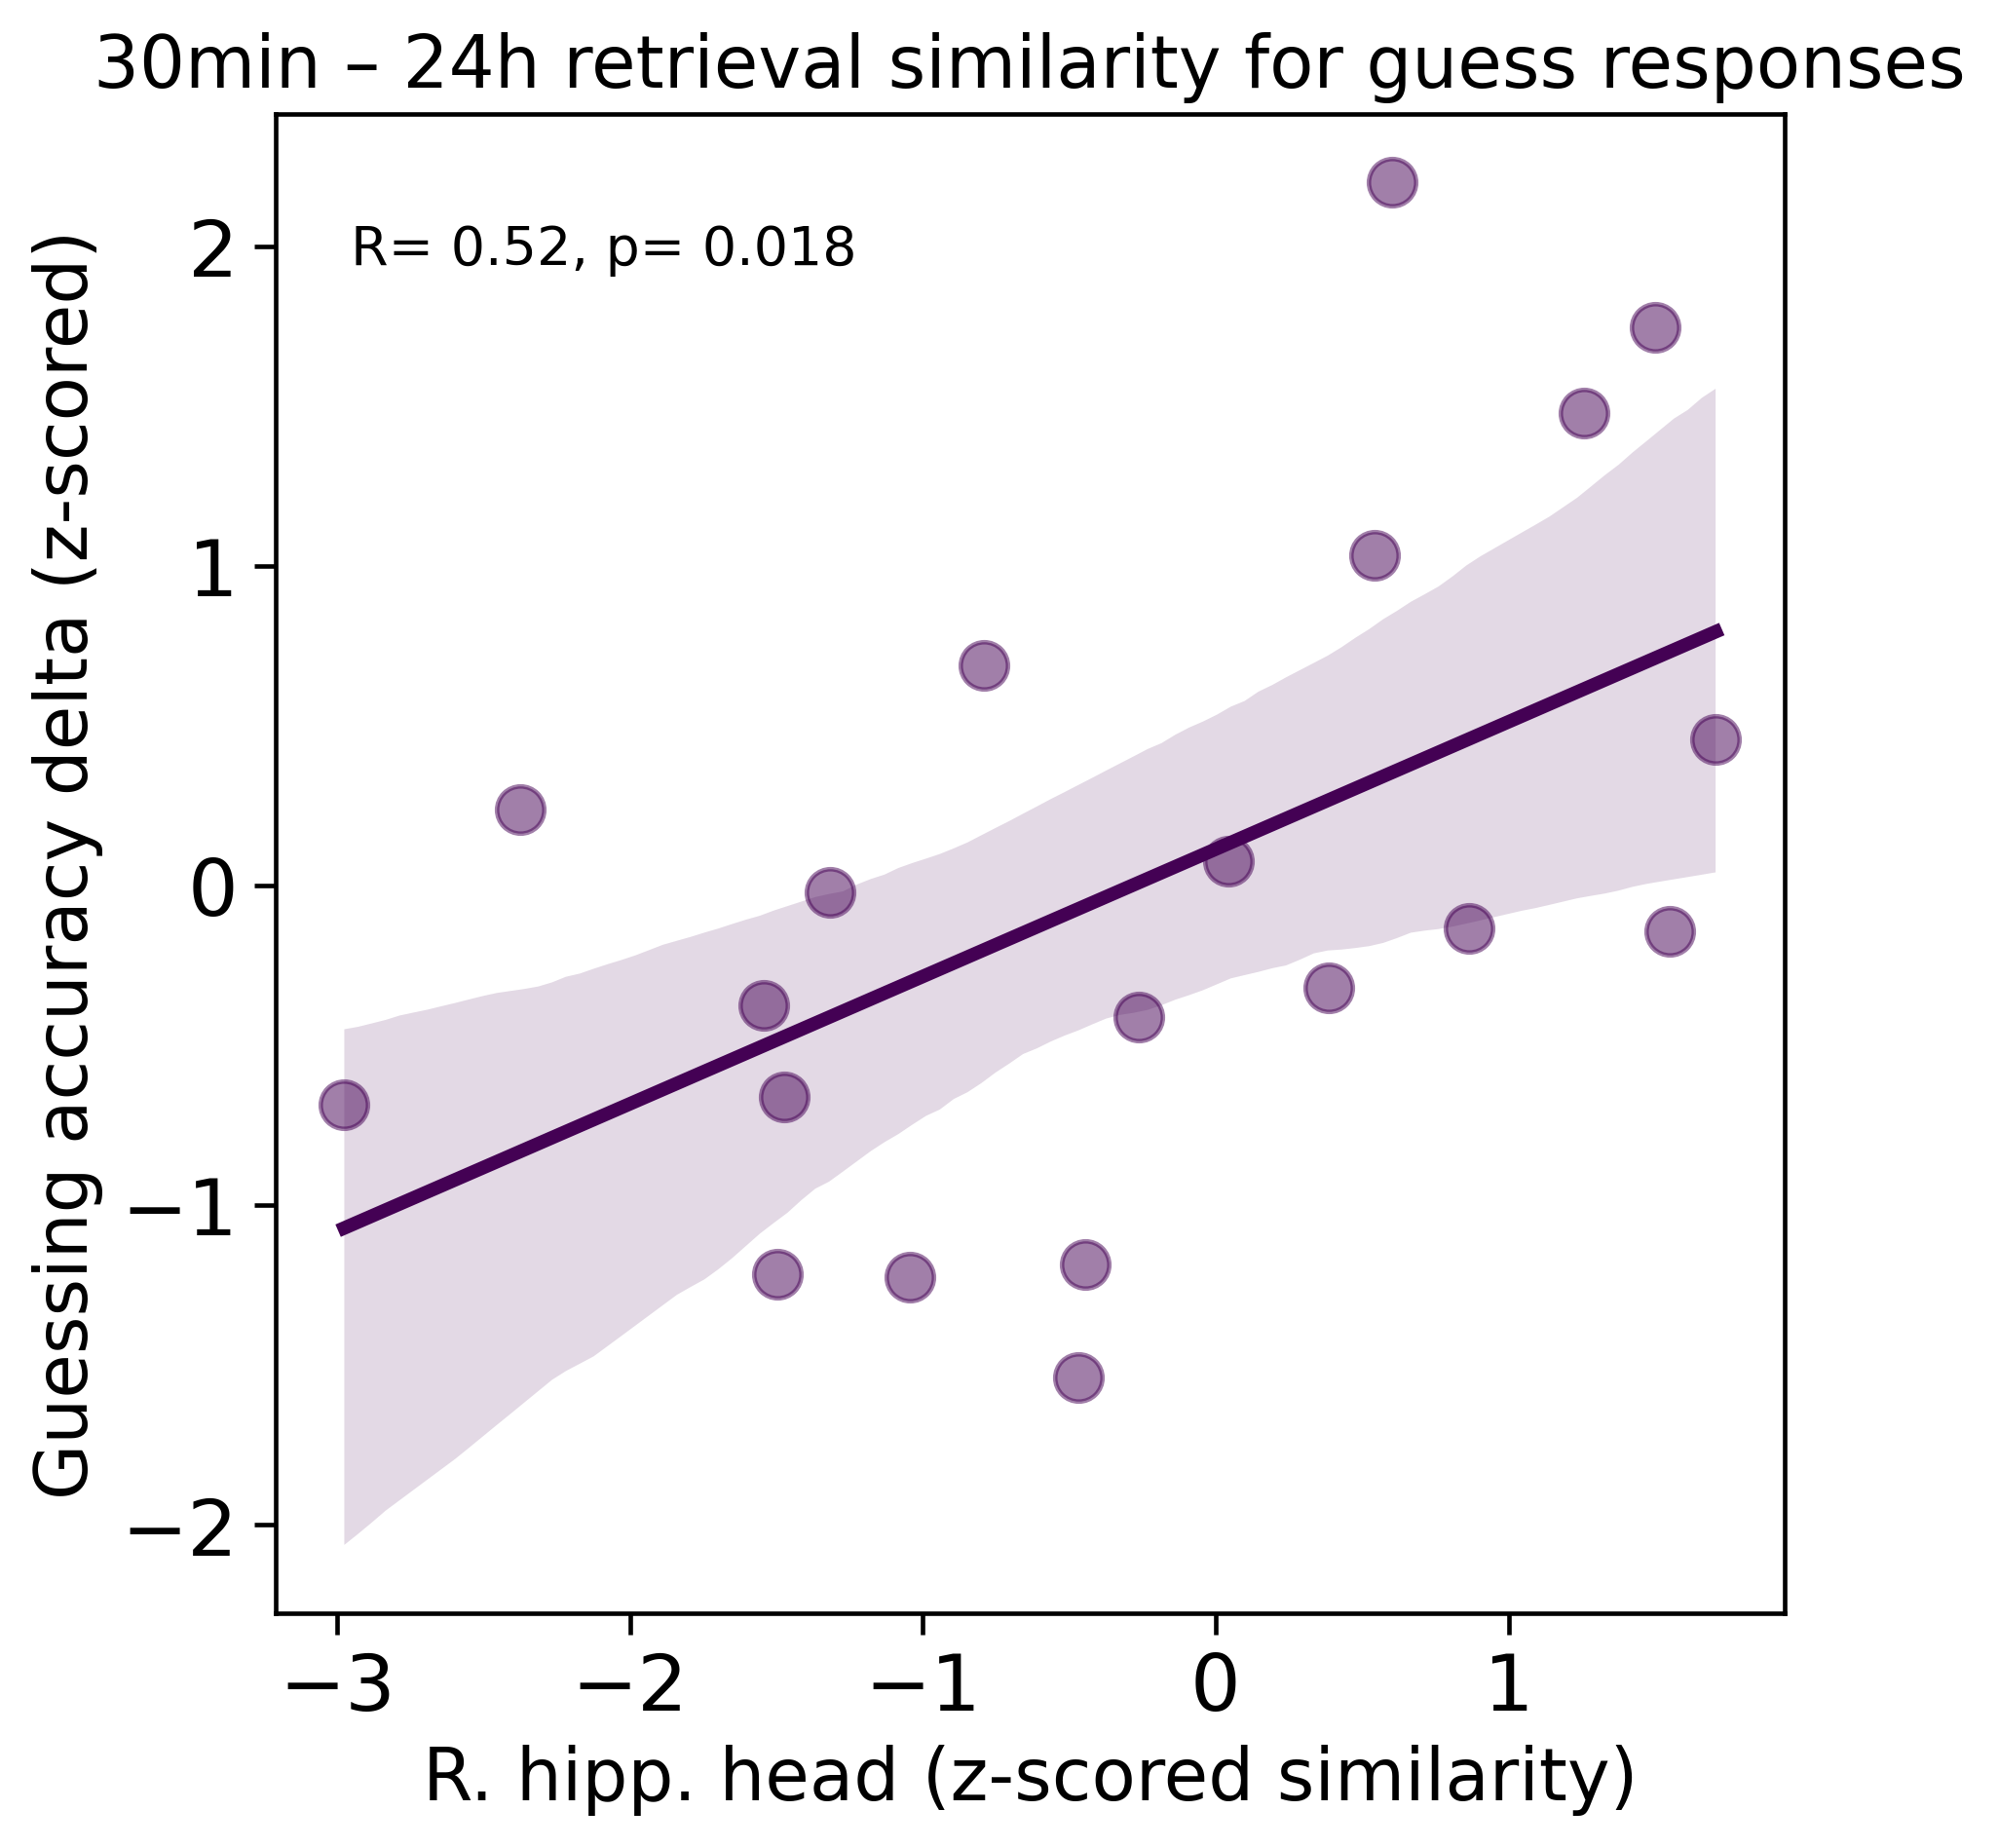
\includegraphics[width=\linewidth/2]{paper/src/figures/20240530_hipp-array_n_ret1_ret2_perm_consc_unconsc_corr-unconsc_incorr_R. hipp. head_ERS_correl.png}
     \caption*{\textbf{Figure S4. Similarity of voxel patterns between the 30-minute and the 24-hour category retrieval are relevant for the accuracy of guess responses.} \\ \vspace{0.5em}
Retrieval-retrieval similarity of voxel patterns in the right hippocampal head underlying correct guess responses revealed a non-significant mean value comparison but a significant between-subjects correlation with the delta of correct guess responses (i.e., number of correct guess responses at 24 hours minus number of correct guess responses at 30 minutes, p = 0.018, R = 0.52, B\textsubscript{10} = 3.7). Results presented in this panel were acquired with the small FOV fMRI sequence. Abbreviations: R., right; hipp., hippocampus.}
\end{figure}



\newpage

 \begin{figure}[!ht]
    \centering
\begin{subfigure}[]{0.6\linewidth}
    \centering
    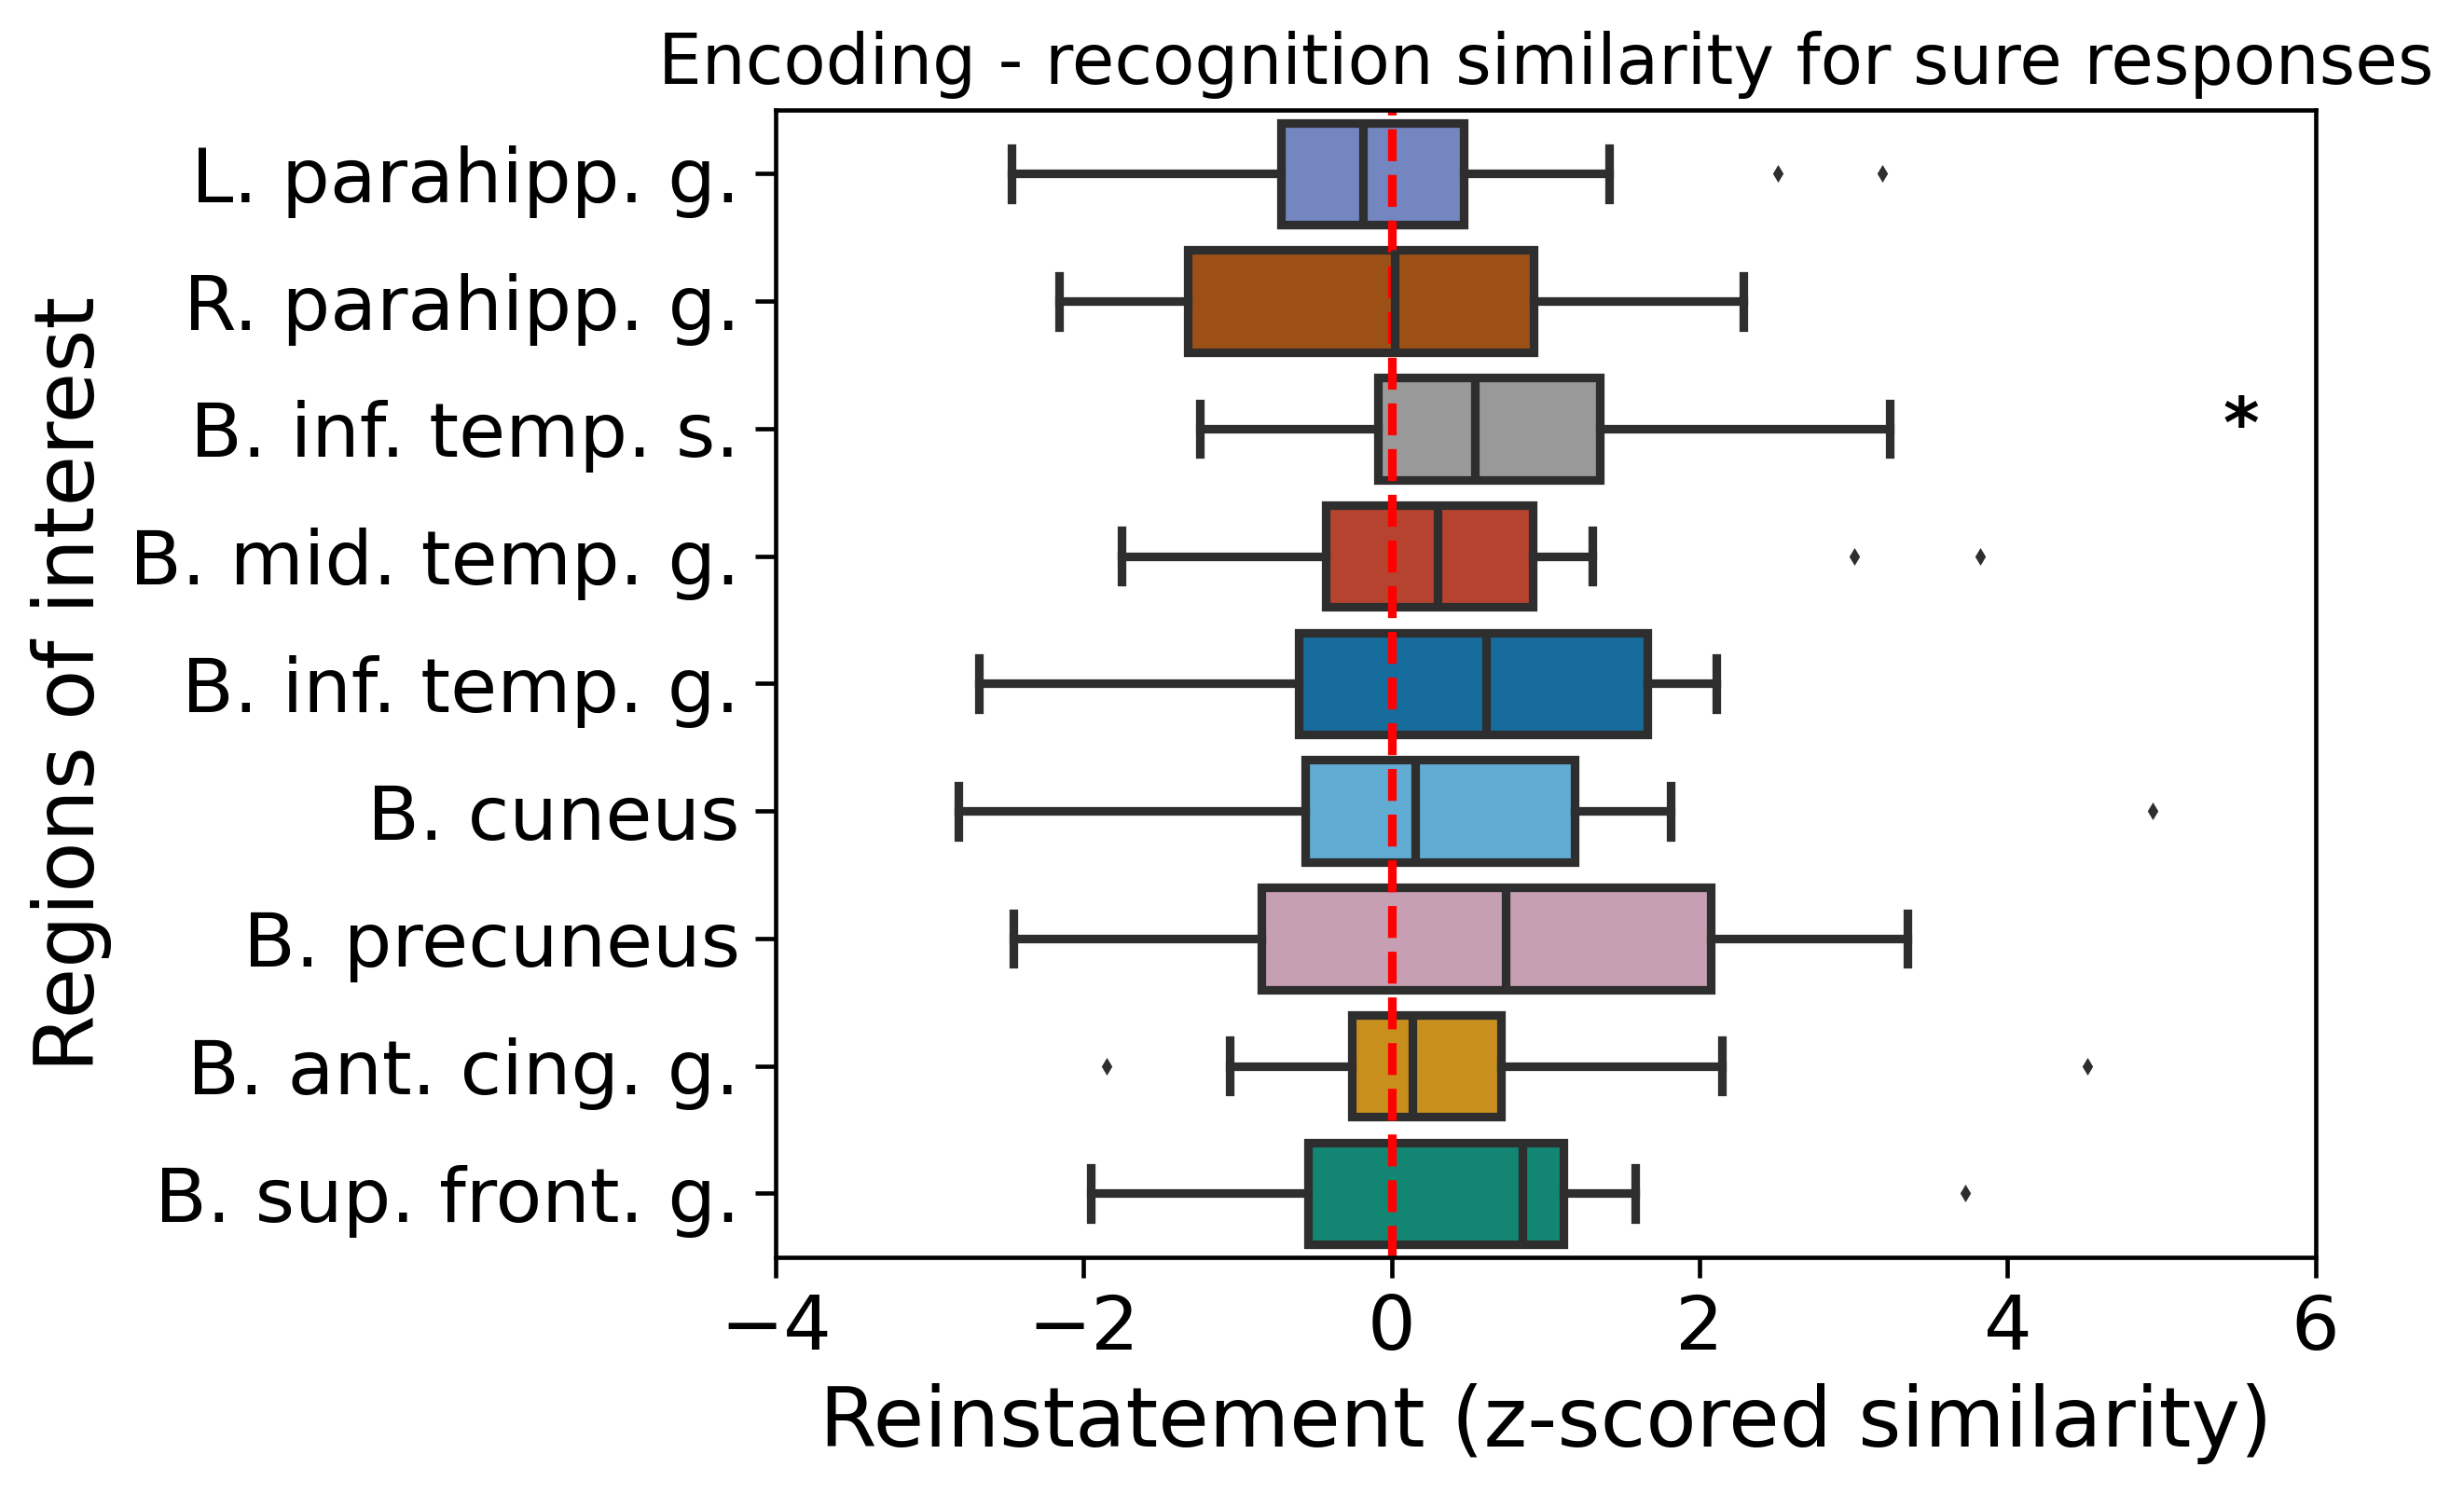
\includegraphics[width=\linewidth]{paper/src/figures/20240710_wb-all_memory_n_enc_recog_perm_consc_consc-unconsc_incorr.png}
\end{subfigure}
\begin{subfigure}[]{0.19\linewidth}
    \centering
    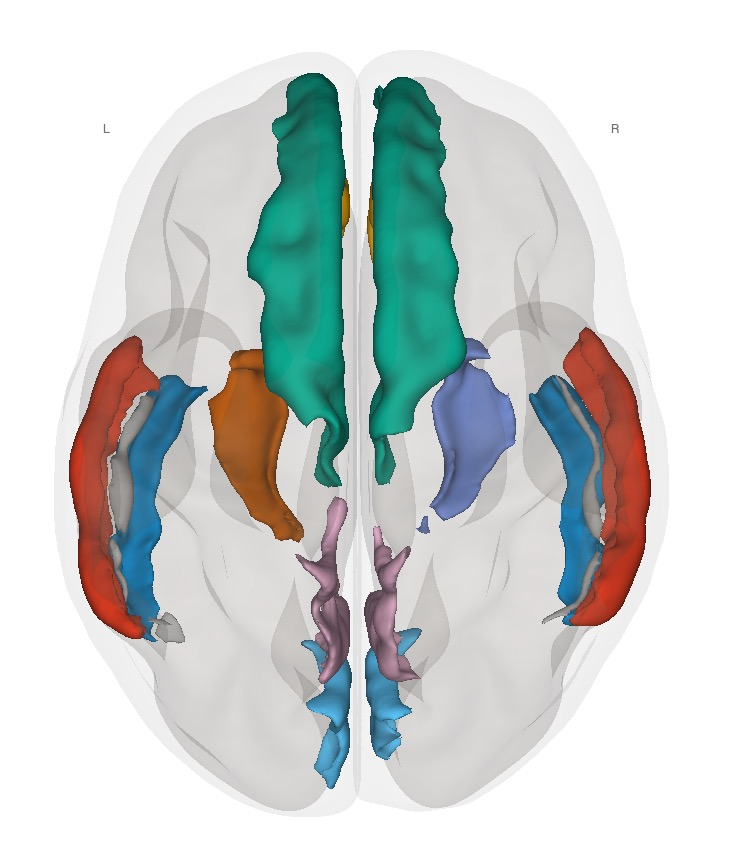
\includegraphics[width=\linewidth]{paper/src/figures/wb_rois_top.jpg}
\end{subfigure}
\begin{subfigure}[]{0.19\linewidth}
    \centering
    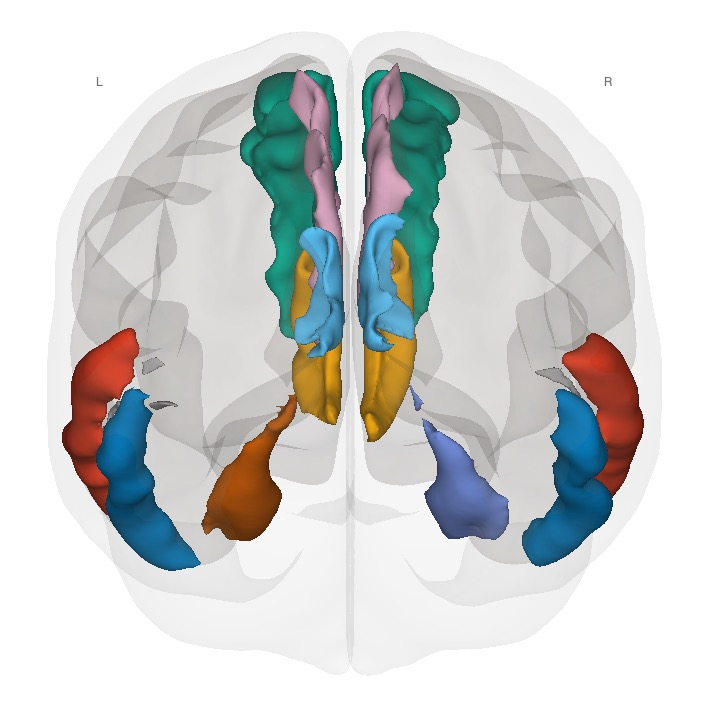
\includegraphics[width=\linewidth]{paper/src/figures/wb_rois_back.jpg}
\end{subfigure}
     \caption*{\textbf{Figure S5. Similarity of voxel patterns between encoding and recognition at 24 hours was relevant for retrieval success.} \\ \vspace{0.5em}
Significant mean value comparison in bilateral inferior temporal sulcus regarding correct sure responses (p = 0.026, t(17) = 2.55, B\textsubscript{10} = 2.9). Results presented in this panel were acquired with the whole-brain fMRI sequence. *p < 0.05, **p < 0.01 by Student’s t test. Abbreviations: R., right; L., left; B., bilateral; parahipp., parahippocampus; inf., inferior; mid., middle; ant., anterior; cing., cingulate; sup., superior; front., frontal; s., sulcus, g., gyrus.
}
\end{figure}


\newpage


 \begin{figure}[!ht]
    \centering
     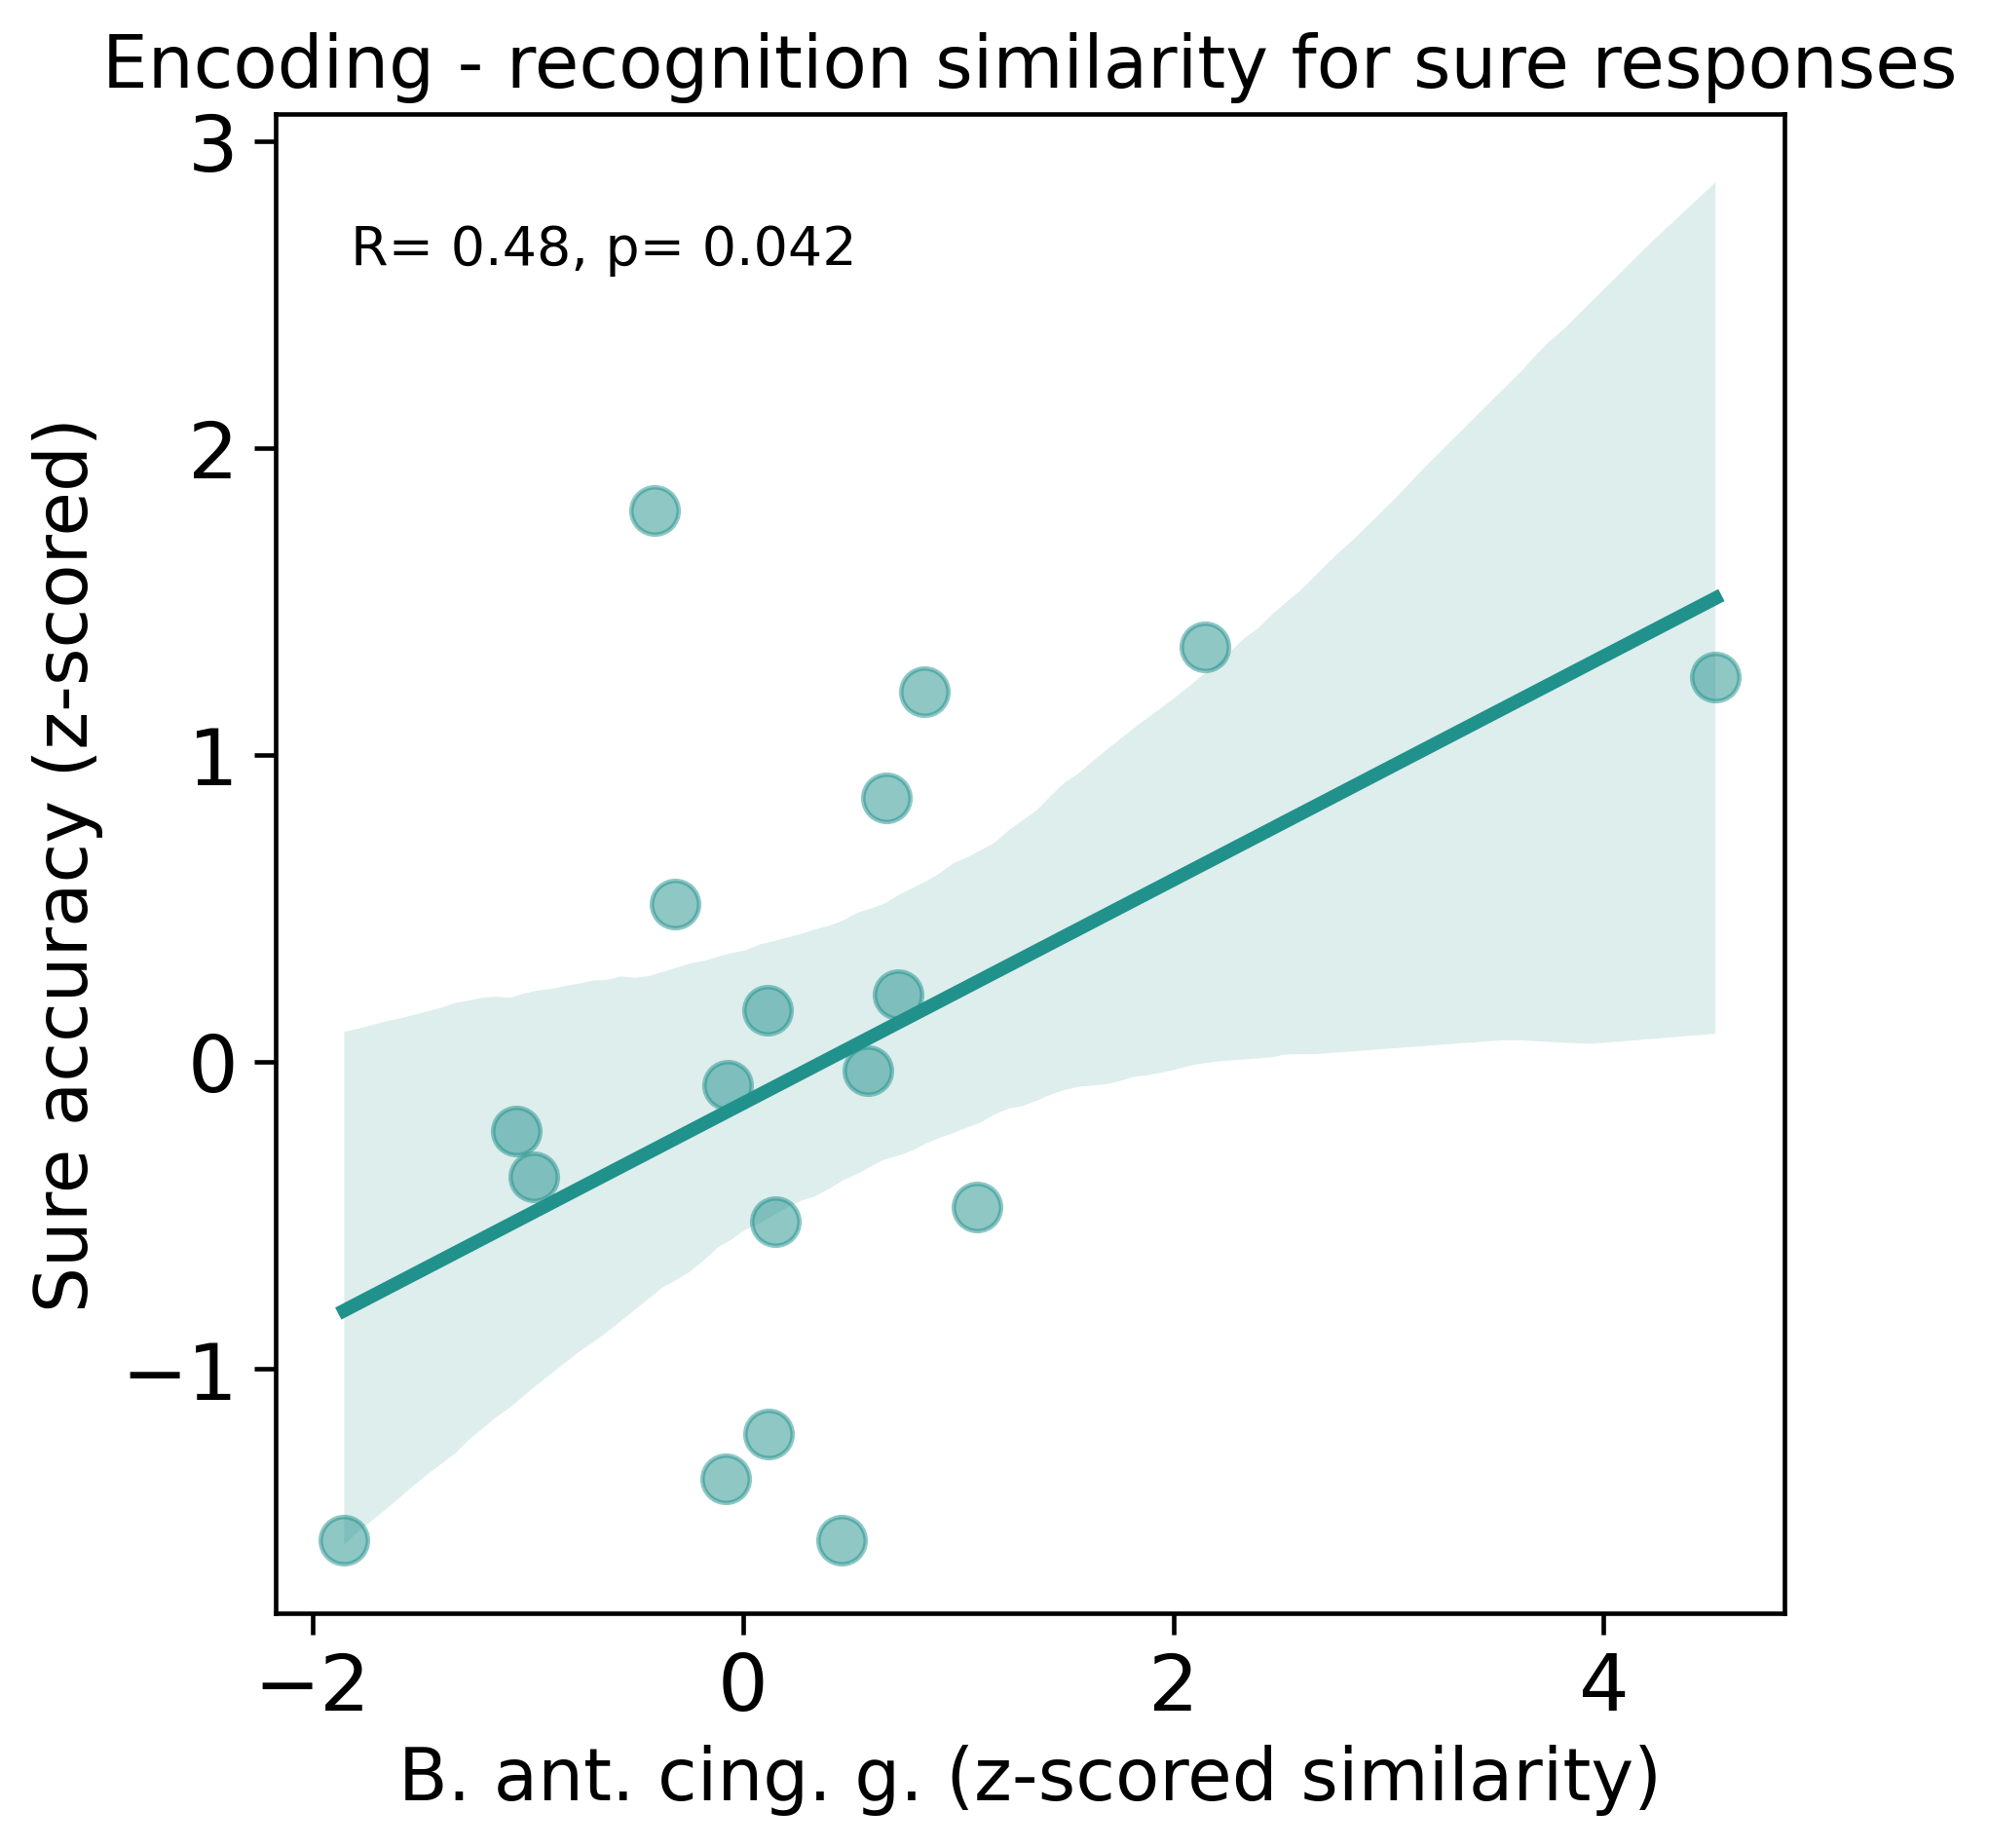
\includegraphics[width=\linewidth/2]{paper/src/figures/20240710_wb-all_memory_n_enc_recog_perm_consc_consc-unconsc_incorr_B. ant. cing. g._ERS_correl.png}
     \caption*{\textbf{Figure S6. Similarity of voxel patterns between encoding and recognition at 24 hours was relevant for retrieval success.} \\ \vspace{0.5em}
 Pattern similarity in bilateral anterior cingulate gyrus (B. ant. cing. g.) underlying correct sure responses revealed a non-significant mean value comparison but a significant between-subjects correlation with the number of correct sure responses given on the recognition task (p = 0.041, R = 0.48, B\textsubscript{10} = 2.0).  Results presented in this panel were acquired with the small FOV fMRI sequence. Abbreviations: B., bilateral; ant., anterior; cing., cingulate; g., gyrus.}
\end{figure}


\newpage
\section{Supplementary Tables}
%----- Requires booktabs package -----%
\begin{table}[ht]
	
	\label{tab:aNCOVA-Mean_acc_bysub}
	{
		\begin{tabular}{lrrrrr}
			\toprule
			Cases & Sum of Squares & df & Mean Square & F & p  \\
			\cmidrule[0.4pt]{1-6}
			Repetition & $0.002$ & $1$ & $0.002$ & $0.041$ & $0.840$  \\
			n & $0.050$ & $1$ & $0.050$ & $1.106$ & $0.296$  \\
			Residuals & $3.464$ & $77$ & $0.045$ & ~ & ~  \\
			\bottomrule
			% \addlinespace[1ex]
			% \multicolumn{6}{p{0.5\linewidth}}{\textit{Note.} Type III Sum of Squares} \\
		\end{tabular}
        \vspace{1em}
        \caption{\textbf{Additional analysis regarding guessing accuracy during the recognition task, related to Figure 2.}\\ 
        Since objects were repeatedly shown during the recognition task (see STAR Methods), it was theoretically possible to answer recognition trials correctly solely based on previous choices for these objects, while still rating them as guess answers. No participant reported to have done so. Still, we investigated if responses for repeated objects would contribute differently to guessing accuracy than responses for first presentations of the objects (within the recognition task). In addition, we included the number of guessed responses as a covariate, because it varied considerably across participants.
        The table shows the result of an analysis of covariance (ANCOVA) which shows that it is unlikely that repeated objects (case: repetition) contributed differently to guessed retrieval accuracy, and that number of guessed responses (case: n) was not associated with guessing accuracy across participants.}
	}
\end{table}

\label{ancova_source}
\begin{landscape}
\begin{table}[!ht]
    \vspace*{-4cm}
    \raggedright
        \begin{tabular}{ll|cccc|cccc|ccc} \\ \hline
        \multicolumn{2}{l}{\textbf{Anatomical description}} & \multicolumn{4}{c}{\textbf{Cluster}} & \multicolumn{4}{c}{\textbf{Peak}} &  \multicolumn{3}{c}{\textbf{MNI}} \\ \hline
        \multicolumn{2}{l}{\textbf{}} & \multicolumn{1}{l}{p(FWE-corr)} & p(FDR-corr) & k & \multicolumn{1}{l}{p(unc)} & p(FWE-corr) & p(FDR-corr) & T & \multicolumn{1}{l}{p(unc)} & x & y & z \\ \hline
        \textbf{R} & Hippocampus & 0.692 & 0.920 & 128 & 0.120 & 0.472 & 0.519 & 4.05 & 0.000 & 30 & -32 & -9 \\
        \textbf{L} & Posterior cingulate gyrus & 0.998 & 0.920 & 13 & 0.630 & 0.999 & 0.963 & 3.25 & 0.001 & -9 & -52 & 4 \\ \hline
    \end{tabular}
    \vspace{1.0 em}
    \caption{\textbf{Common hippocampal and neocortical areas mediated correct sure and correct guess responses at the 30-minute category retrieval, related to Figure 3A.} \\ 
    This table shows the results of a conjunction analysis for guessed correct > guessed incorrect and sure correct > guessed incorrect trials during 30-min category retrieval. 
    This analysis displays the shared brain activation patterns for guessed correct and sure correct trials. \\ 
    \vspace{1.0 em} \textit{Notes}. Results from small FOV fMRI sequence. Threshold set to p < .001, k = 10 voxels, uncorrected. MNI, Montreal Neurological Institute; FWE-corr, family wise error corrected; FDR-corr, false discovery rate corrected; unc, uncorrected; g, gyrus; k, cluster size in number of voxels; L, left hemisphere; R, right hemisphere; B, bilateral.}
    \label{tab:Retrieval1_hipp_Conjunction_ConsciousUnconscious}
\end{table}
\end{landscape}


\begin{landscape}
\begin{table}[!ht]
    \vspace*{-4cm}
    \raggedright
       \begin{tabular}{ll|cccc|cccc|ccc} \\ \hline
        \multicolumn{2}{l}{\textbf{Anatomical description}} & \multicolumn{4}{c}{\textbf{Cluster}} & \multicolumn{4}{c}{\textbf{Peak}} &  \multicolumn{3}{c}{\textbf{MNI}} \\ \hline
        \multicolumn{2}{l}{\textbf{}} & \multicolumn{1}{l}{p(FWE-corr)} & p(FDR-corr) & k & \multicolumn{1}{l}{p(unc)} & p(FWE-corr) & p(FDR-corr) & T & \multicolumn{1}{l}{p(unc)} & x & y & z \\ \hline
        \textbf{L} & Lingual gyrus & 0.996 & 0.920 & 18 & 0.563 & 0.999 & 0.985 & 3.28 & 0.001 & -16 & -54 & 1 \\
        \textbf{L} & Posterior cingulate gyrus& 1.000 & 0.920 & 2 & 0.876 & 1.000 & 0.985 & 3.16 & 0.001 & -11 & -45 & -1 \\
        \textbf{L} & Lingual gyrus & 1.000 & 0.920 & 1 & 0.920 & 1.000 & 0.985 & 3.13 & 0.001 & -17 & -55 & 2 \\ \hline
    \end{tabular}
    \vspace{1.0 em}
    \caption{\textbf{Common neocortical areas mediated correct sure and correct guess responses at the 24-hour category retrieval, related to Figure 3B.}\\
    This table shows the results of a conjunction analysis for guessed correct > guessed incorrect and sure correct > guessed incorrect trials during 24-hour category retrieval. 
    This analysis displays the shared brain activation patterns for guessed correct and sure correct trials. \\
    \vspace{1.0 em} \textit{Notes}. Results from small FOV fMRI sequence. Threshold set to p < .001, k = 10 voxels. MNI, Montreal Neurological Institute; FWE-corr, family wise error corrected; FDR-corr, false discovery rate corrected; unc, uncorrected; g, gyrus; k, cluster size in number of voxels; L, left hemisphere; R, right hemisphere; B, bilateral.}
\label{tab:Retrieval2_hipp_Conjunction_ConsciousUnconscious}
\end{table}
\end{landscape}


\begin{landscape}
\begin{table}[!ht]
    \vspace*{-4cm}
    \raggedright
    \begin{tabular}{ll|cccc|cccc|ccc} \\ \hline
        \multicolumn{2}{l}{\textbf{Anatomical description}} & \multicolumn{4}{c}{\textbf{Cluster}} & \multicolumn{4}{c}{\textbf{Peak}} &  \multicolumn{3}{c}{\textbf{MNI}} \\ \hline
        \multicolumn{2}{l}{\textbf{}} & \multicolumn{1}{l}{p(FWE-corr)} & p(FDR-corr) & k & \multicolumn{1}{l}{p(unc)} & p(FWE-corr) & p(FDR-corr) & T & \multicolumn{1}{l}{p(unc)} & x & y & z \\ \hline
        \textbf{R} & Hippocampus & 0.0188 & 0.0734 & 431 & 0.0012 & 0.1792 & 0.4407 & 6.3158 & 0.0000 & 27 & -8 & -25 \\ 
        \textbf{L} & Ventral diencephalon & 0.1765 & 0.2571 & 227 & 0.0127 & 0.2362 & 0.4407 & 6.1201 & 0.0000 & -16 & -14 & -13 \\ 
        \textbf{R} & Middle temporal g. & 0.4410 & 0.3754 & 147 & 0.0382 & 0.2712 & 0.4407 & 6.0196 & 0.0000 & 48 & -49 & 14 \\ 
        \textbf{R} & Ventral diencephalon & 0.3373 & 0.3186 & 171 & 0.0270 & 0.2881 & 0.4407 & 5.9748 & 0.0000 & 1 & -18 & -11 \\ 
        \textbf{L} & Inferior temporal g. & 0.9870 & 0.8894 & 35 & 0.2852 & 0.3332 & 0.4407 & 5.8651 & 0.0000 & -56 & -10 & -35 \\ 
        \textbf{L} & Inferior temporal g. & 0.3259 & 0.3186 & 174 & 0.0259 & 0.7606 & 0.8631 & 5.0893 & 0.0000 & -44 & -27 & -22 \\ 
        \textbf{R} & Middle temporal g. & 0.9551 & 0.8894 & 50 & 0.2037 & 0.8645 & 0.8631 & 4.8843 & 0.0001 & 59 & -9 & -32 \\ 
        \textbf{R} & Precunues & 0.9457 & 0.8894 & 53 & 0.1912 & 0.8899 & 0.8631 & 4.8239 & 0.0001 & 4 & -64 & 18 \\ 
        \textbf{L} & Posterior cingulate g. & 0.9842 & 0.8894 & 37 & 0.2720 & 0.9171 & 0.8631 & 4.7497 & 0.0001 & -5 & -51 & 12 \\ 
        \textbf{R} & Middle temporal g. & 0.9809 & 0.8894 & 39 & 0.2597 & 0.9184 & 0.8631 & 4.7459 & 0.0001 & 64 & -56 & 8 \\ 
        \textbf{L} & Middle temporal g. & 0.9870 & 0.8894 & 35 & 0.2852 & 0.9478 & 0.8631 & 4.6455 & 0.0001 & -52 & -14 & -25 \\ 
        \textbf{R} & Hippocampus & 0.9551 & 0.8894 & 50 & 0.2037 & 0.9524 & 0.8631 & 4.6264 & 0.0001 & 16 & -39 & 6 \\ 
        \textbf{L} & Middle temporal g. & 0.1806 & 0.2571 & 225 & 0.0131 & 0.9535 & 0.8631 & 4.6219 & 0.0001 & -54 & -19 & -15 \\ 
        \textbf{} & Brain Stem & 0.5792 & 0.4788 & 121 & 0.0568 & 0.9714 & 0.8631 & 4.5312 & 0.0001 & 0 & -24 & -20 \\ 
        \textbf{L} & Middle temporal g. & 0.6320 & 0.4839 & 112 & 0.0656 & 0.9716 & 0.8631 & 4.5300 & 0.0001 & -68 & -28 & -16 \\ 
        \textbf{L} & Ventral diencephalon & 0.9968 & 0.8894 & 24 & 0.3770 & 0.9991 & 0.9201 & 4.1062 & 0.0003 & -11 & -18 & -16 \\ 
        \textbf{L} & Middle temporal g. & 0.9895 & 0.8894 & 33 & 0.2993 & 0.9994 & 0.9201 & 4.0704 & 0.0004 & -58 & -29 & -10 \\ \hline
    
    \end{tabular}
    \vspace{1.0 em}
    \caption{\textbf{Activity in hippocampus and episodic memory network underlying correct guess responses correlated with the guessing accuracy on the category retrieval task at 30 minutes, related to Figure 3C.} \\ 
    This table shows the results of a brain-behavior correlation for correct > incorrect guess responses correlated with guessed retrieval performance at 30-minute retrieval. This analysis displays brain activation during 30-min retrieval that was modulated by guessed retrieval performance at 30-min retrieval. \\ 
    \vspace{1.0 em} \textit{Notes}. Results from small FOV fMRI sequence. Threshold set to p < .001, k = 10 voxels. MNI, Montreal Neurological Institute; FWE-corr, family wise error corrected; FDR-corr, false discovery rate corrected; unc, uncorrected; g, gyrus; k, cluster size in number of voxels; L, left hemisphere; R, right hemisphere; B, bilateral; ROI, region of interest.}
    \label{tab:unconsciousCORR_Day1}
\end{table}
\end{landscape}


\begin{landscape}
\begin{table}[!ht]
    \vspace*{-4cm}
    \raggedright
\begin{tabular}{ll|cccc|cccc|ccc} \\ \hline
        \multicolumn{2}{l}{\textbf{Anatomical description}} & \multicolumn{4}{c}{\textbf{Cluster}} & \multicolumn{4}{c}{\textbf{Peak}} &  \multicolumn{3}{c}{\textbf{MNI}} \\ \hline
        \multicolumn{2}{l}{\textbf{}} & \multicolumn{1}{l}{p(FWE-corr)} & p(FDR-corr) & k & \multicolumn{1}{l}{p(unc)} & p(FWE-corr) & p(FDR-corr) & T & \multicolumn{1}{l}{p(unc)} & x & y & z \\ \hline
        \textbf{R} & Middle temporal gyrus & 0.528 & 0.544 & 148 & 0.060 & 0.320 & 0.775 & 5.77 & 0.000 & 60 & -24 & -11 \\
        \textbf{R} & Hippocampus & 0.814 & 0.544 & 89 & 0.135 & 0.421 & 0.775 & 5.55 & 0.000 & 31 & -36 & -6 \\
        %\textbf{L} & Cerebral white matter & 0.686 & 0.544 & 115 & 0.093 & 0.825 & 0.775 & 4.84 & 0.000 & -43.6 & -54.8 & 1.6 \\
        \textbf{R} & Hippocampus & 0.931 & 0.563 & 60 & 0.214 & 0.890 & 0.775 & 4.70 & 0.000 & 28 & -10 & -28 \\
        \textbf{R} & Middle temporal gyrus & 0.997 & 0.715 & 20 & 0.477 & 0.908 & 0.775 & 4.65 & 0.000 & 68 & -22 & -18 \\
        \textbf{L} & Temporal pole & 0.851 & 0.544 & 81 & 0.152 & 0.941 & 0.775 & 4.55 & 0.000 & -36 & 4 & -29 \\
        \textbf{R} & Middle temporal gyrus & 0.995 & 0.715 & 25 & 0.423 & 0.955 & 0.775 & 4.49 & 0.000 & 56 & -16 & -15 \\
        %\textbf{L} & Cerebral white matter & 0.884 & 0.544 & 73 & 0.173 & 0.957 & 0.775 & 4.48 & 0.000 & -29.2 & -38.8 & 8.0 \\
        \textbf{R} & Middle temporal gyrus & 0.974 & 0.612 & 43 & 0.291 & 0.968 & 0.775 & 4.43 & 0.000 & 61 & -16 & -16 \\
        \textbf{} & Brain stem & 0.833 & 0.544 & 85 & 0.143 & 0.980 & 0.775 & 4.35 & 0.000 & -2 & -36 & -10 \\
        \textbf{L} & Hippocampus & 0.968 & 0.612 & 46 & 0.275 & 0.991 & 0.775 & 4.24 & 0.000 & -17 & -40 & 3 \\
        \textbf{L} & Middle temporal gyrus & 0.896 & 0.544 & 70 & 0.181 & 0.992 & 0.775 & 4.21 & 0.000 & -52 & -46 & 4 \\
        \textbf{} & Brain stem & 0.997 & 0.715 & 22 & 0.454 & 0.996 & 0.775 & 4.14 & 0.000 & 9 & -19 & -27 \\
       % \textbf{R} & Cerebral white matter & 0.993 & 0.715 & 28 & 0.396 & 1.000 & 0.786 & 3.91 & 0.001 & 55.6 & -44.4 & 2.4 \\ \hline
    \end{tabular}
    \vspace{1.0 em}
    \caption{\textbf{Hippocampal and middle temporal gyrus activity underlying correct guess responses correlated with the guessing accuracy on the category retrieval task at 24 hours, related to Figure 3C.} \\ 
    This table shows the results of a brain-behavior correlation for correct > incorrect guess responses that correlated with guessed retrieval performance at 24-hour retrieval.
    This analysis displays brain activation during 24-hour guessed retrieval that was modulated by guessed retrieval performance. \\
    \vspace{1.0 em} \textit{Notes}. Results from small FOV fMRI sequence. Clusters identified solely within white matter regions have been excluded. Threshold set to p < .001, k = 10 voxels. MNI, Montreal Neurological Institute; FWE-corr, family wise error corrected; FDR-corr, false discovery rate corrected; unc, uncorrected; g, gyrus; k, cluster size in number of voxels; L, left hemisphere; R, right hemisphere; B, bilateral; ROI, region of interest.}
    \label{tab:unconsciousCORR_Day2}
\end{table}
\end{landscape}
\begin{landscape}
\begin{table}[!ht]
    \vspace*{-4cm}
    \raggedright
    \footnotesize
\begin{tabular}{ll|cccc|cccc|ccc} \\ \hline
        \multicolumn{2}{l}{\textbf{Anatomical description}} & \multicolumn{4}{c}{\textbf{Cluster}} & \multicolumn{4}{c}{\textbf{Peak}} &  \multicolumn{3}{c}{\textbf{MNI}} \\ \hline
        \multicolumn{2}{l}{\textbf{}} & \multicolumn{1}{l}{p(FWE-corr)} & p(FDR-corr) & k & \multicolumn{1}{l}{p(unc)} & p(FWE-corr) & p(FDR-corr) & T & \multicolumn{1}{l}{p(unc)} & x & y & z \\ \hline
        \textbf{B} & Anterior cingulate g. \& medial superior frontal g. & 0.000 & 0.000 & 86 & 0.000 & 0.042 & 0.363 & 7.81 & 0.000 & 12 & 42 & -4 \\
        \textbf{} & & & & & & 1.000 & 0.918 & 4.69 & 0.000 & 12 & 42 & 10 \\
        %\textbf{R} & Cerebral white matter & 0.039 & 0.014 & 29 & 0.000 & 0.095 & 0.363 & 7.36 & 0.000 & 12 & -80 & 20 \\
        %\textbf{R} & Cerebral white matter & 0.929 & 0.132 & 10 & 0.017 & 0.347 & 0.474 & 6.68 & 0.000 & 2 & -38 & 14 \\
        \textbf{R} & Precuneus & 0.704 & 0.083 & 13 & 0.008 & 0.400 & 0.474 & 6.61 & 0.000 & 14 & -48 & 52 \\
        %\textbf{L} & Cerebral white matter & 0.868 & 0.127 & 11 & 0.013 & 0.786 & 0.474 & 6.27 & 0.000 & -48 & -22 & 28 \\
        %\textbf{L} & Cerebral white matter & 0.704 & 0.083 & 13 & 0.008 & 0.849 & 0.474 & 6.23 & 0.000 & -44 & -40 & -8 \\
        %\textbf{L} & Cerebral white matter & 0.013 & 0.007 & 35 & 0.000 & 0.946 & 0.474 & 6.18 & 0.000 & -24 & -28 & 32 \\
        \textbf{L} & Medial superior frontal g. & 0.929 & 0.132 & 10 & 0.017 & 0.958 & 0.474 & 6.12 & 0.000 & -6 & 34 & 30 \\
        %\textbf{L} & Cerebral white matter & 0.614 & 0.077 & 14 & 0.006 & 0.978 & 0.474 & 6.00 & 0.000 & -30 & -42 & 24 \\
        \textbf{L} & Middle cingulate gyrus & 0.000 & 0.000 & 60 & 0.000 & 0.986 & 0.479 & 5.93 & 0.000 & -6 & -22 & 34 \\
        \textbf{} & & & & & & 1.000 & 0.853 & 5.10 & 0.000 & 6 & -22 & 42 \\
        \textbf{} & & & & & & 1.000 & 0.897  & 4.89 & 0.000 & -12 & -32 & 42 \\
        \textbf{R} & Anterior cingulate gyrus & 0.704 & 0.083 & 13 & 0.008 & 0.995 & 0.541 & 5.79 & 0.000 & 8 & 34 & 6 \\
        \textbf{R} & Cuneus & 0.704 & 0.083 & 13 & 0.008 & 0.998 & 0.589 & 5.67 & 0.000 & 4 & -82 & 6 \\
        \textbf{R} & Precuneus & 0.262 & 0.052 & 19 & 0.002 & 1.000 & 0.827 & 5.40 & 0.000 & 12 & -60 & 26 \\
        %\textbf{L} & Cerebral white matter & 0.217 & 0.052 & 20 & 0.002 & 1.000 & 0.827 & 5.38 & 0.000 & -46 & -6 & -22 \\
        \textbf{} & Cerebellar vermal lobules & 0.448 & 0.063 & 16 & 0.004 & 1.000 & 0.853 & 5.27 & 0.000 & 4 & -46 & -18 \\
        \textbf{} & Brain stem & 0.377 & 0.057 & 17 & 0.003 & 1.000 & 0.853 & 5.25 & 0.000 & -2 & -32 & -6 \\
        \textbf{L} & Precuneus & 0.377 & 0.057 & 17 & 0.003 & 1.000 & 0.853 & 5.23 & 0.000 & -8 & -60 & 34 \\
        \textbf{} & & & & & & 1.000 & 0.897 & 4.75 & 0.000 & -14 & -64 & 42 \\
        \textbf{L} & Precuneus & 0.614 & 0.077 & 14 & 0.006 & 1.000 & 0.853 & 5.13 & 0.000 & -20 & -58 & 24 \\
        \textbf{L} & Middle cingulate gyrus & 0.528 & 0.067 & 15 & 0.005 & 1.000 & 0.853 & 5.12 & 0.000 & -8 & 0 & 36 \\
        \textbf{L} & Lingual gyrus & 0.148 & 0.045 & 22 & 0.001 & 1.000 & 0.853 & 5.03 & 0.000 & -14 & -54 & 0 \\
        \textbf{} & & & & & & 1.000 & 0.953 & 4.09 & 0.000 & -4 & -52 & 4 \\
        \textbf{L} & Precuneus & 0.262 & 0.052 & 19 & 0.002 & 1.000 & 0.853 & 5.01 & 0.000 & -12 & -54 & 20 \\
        \textbf{L} & Hippocampus & 0.868 & 0.127 & 11 & 0.013 & 1.000 & 0.853 & 5.00 & 0.000 & -34 & -28 & -10 \\
        \textbf{} & & & & & & 1.000 & 0.953 & 4.11 & 0.000 & -28 & -32 & -6 \\
        \textbf{L} & Posterior cingulate gyrus & 0.315 & 0.057 & 18 & 0.002 & 1.000 & 0.875 & 4.97 & 0.000 & -2 & -44 & 24 \\
        \textbf{L} & Cuneus & 0.929 & 0.132 & 10 & 0.017 & 1.000 & 0.897 & 4.81 & 0.000 & 0 & -84 & 36 \\
        \textbf{L} & Anterior cingulate gyrus & 0.262 & 0.052 & 19 & 0.002 & 1.000 & 0.897 & 4.75 & 0.000 & -12 & 42 & 8 \\
        \textbf{L} & Thalamus & 0.929 & 0.132 & 10 & 0.017 & 1.000 & 0.897 & 4.75 & 0.000 & -18 & -24 & 10 \\
        %\textbf{R} & Cerebral white matter & 0.528 & 0.067 & 15 & 0.005 & 1.000 & 0.918 & 4.72 & 0.000 & 18 & -30 & 46 \\
        \textbf{R} & Lingual gyrus & 0.016 & 0.007 & 34 & 0.000 & 1.000 & 0.918 & 4.59 & 0.000 & 12 & -52 & 2 \\
        %\textbf{L} & Cerebral white matter & 0.528 & 0.067 & 15 & 0.005 & 1.000 & 0.918 & 4.56 & 0.000 & -40 & -16 & 30 \\
        \textbf{R} & Posterior cingulate gyrus & 0.929 & 0.132 & 10 & 0.017 & 1.000 & 0.918 & 4.50 & 0.000 & 4 & -38 & 28 \\
        \textbf{R} & Pallidum  & 0.377 & 0.057 & 17 & 0.003 & 1.000 & 0.918 & 4.47 & 0.000 & 14 & -8 & -4 \\
        \textbf{L} & Anterior insula & 0.929 & 0.132 & 10 & 0.017 & 1.000 & 0.918 & 4.44 & 0.000 & -30 & 20 & -10 \\
        \textbf{L} & Precuneus & 0.448 & 0.063 & 16 & 0.004 & 1.000 & 0.918 & 4.43 & 0.000 & -4 & -46 & 46 \\
        \textbf{} & & & & & & 1.000 & 0.953 & 4.17 & 0.000 & -8 & -44 & 38 \\
        \textbf{R} & Superior frontal gyrus & 0.929 & 0.132 & 10 & 0.017 & 1.000 & 0.945 & 4.25 & 0.000 & 16 & 52 & 34 \\ \hline
    \end{tabular}
    \vspace{1.0 em}
    \caption{\textbf{Hippocampal functional connectivity  during learning correlated with the 30-minute guessing accuracy for forgotten associations, related to Figure 4A.} \\
    This table shows the results of a correlative gPPI analysis with the seed region in the right hippocampus head: learning trials that would yield correct > incorrect guess responses during the 30-minute retrieval (subsequent memory analysis) revealed that connectivity estimates correlated between-subjects with guessing accuracy.
    This analysis displays right hippocampus head functional connectivity during learning that was modulated by subsequent guessing accuracy.\\
    \vspace{1.0 em} \textit{Notes}. Results from whole-brain fMRI sequence. Clusters identified solely within white matter regions have been excluded. Threshold set to p < .001, k = 10 voxels. MNI, Montreal Neurological Institute; FWE-corr, family wise error corrected; FDR-corr, false discovery rate corrected; unc, uncorrected; g, gyrus; gPPI, general psychophysiological interaction; k, cluster size in number of voxels; L, left hemisphere; R, right hemisphere; B, bilateral.}
    \label{tab:Encoding_unconscious_gPPI}
\end{table}
\end{landscape}

\begin{landscape}
\begin{table}[!ht]
    \vspace*{-4cm}
    \raggedright
    \tiny
\begin{tabular}{ll|cccc|ccccc|ccc} \\ \hline
        \multicolumn{2}{l}{\textbf{Anatomical description}} & \multicolumn{4}{c}{\textbf{Cluster}} & \multicolumn{5}{c}{\textbf{Peak}} &  \multicolumn{3}{c}{\textbf{MNI}} \\ \hline
        \multicolumn{2}{l}{} & \textbf{p(FWE-corr)} & \textbf{p(FDR-corr)} & \textbf{k} & \textbf{p(unc)} & \textbf{p(FWE-corr)} & \textbf{p(FDR-corr)} & \textbf{T} & \textbf{Z} & \textbf{p(unc)} & x & y & z \\ \hline
        \textbf{L} & Temporal pole & 0.920 & 0.138 & 10 & 0.016 & 0.014 & 0.327 & 8.41 & 5.29 & 0.000 & -48 & 18 & -22 \\
        %\textbf{R} & Cerebral white matter & 0.504 & 0.082 & 15 & 0.005 & 0.223 & 0.811 & 6.91 & 4.77 & 0.000 & 20 & 28 & 34 \\
        \textbf{L} & Middle frontal gyrus & 0.920 & 0.138 & 10 & 0.016 & 0.336 & 0.811 & 6.70 & 4.69 & 0.000 & -26 & 42 & 16 \\
        \textbf{L} & Inferior temporal gyrus & 0.201 & 0.044 & 20 & 0.001 & 0.393 & 0.811 & 6.62 & 4.65 & 0.000 & -48 & -40 & -32 \\
        \textbf{L} & Caudate & 0.042 & 0.020 & 28 & 0.000 & 0.396 & 0.811 & 6.62 & 4.65 & 0.000 & -16 & -8 & 18 \\
        %\textbf{L} & Cerebral white matter & 0.772 & 0.124 & 12 & 0.010 & 0.507 & 0.811 & 6.49 & 4.60 & 0.000 & -14 & 30 & -8 \\
        %\textbf{L} & Cerebral white matter & 0.136 & 0.034 & 22 & 0.001 & 0.550 & 0.811 & 6.45 & 4.59 & 0.000 & -30 & 14 & 46 \\
        \textbf{R} & Medial superior frontal gyrus & 0.000 & 0.000 & 144 & 0.000 & 0.820 & 0.813 & 6.25 & 4.50 & 0.000 & 12 & 46 & 28 \\
        \textbf{} & & & & & & 1.000 & 0.957 & 5.41 & 4.11 & 0.000 & 8 & 48 & 36 \\
        \textbf{} & & & & & & 1.000 & 0.957 & 5.30 & 4.06 & 0.000 & 6 & 36 & 20 \\
        %\textbf{L} & Cerebral white matter & 0.854 & 0.129 & 11 & 0.012 & 0.955 & 0.813 & 6.16 & 4.46 & 0.000 & 44 & 20 & 16 \\
        \textbf{R} & Medial superior frontal g. & 0.425 & 0.081 & 16 & 0.004 & 0.992 & 0.957 & 5.87 & 4.33 & 0.000 & -4 & 56 & 18 \\
        \textbf{R} & Inferior temporal gyrus & 0.355 & 0.074 & 17 & 0.003 & 0.995 & 0.957 & 5.80 & 4.30 & 0.000 & 54 & -4 & -40 \\
        \textbf{R} & Middle temporal gyrus & 0.092 & 0.034 & 24 & 0.001 & 0.997 & 0.957 & 5.77 & 4.29 & 0.000 & 62 & -42 & 2 \\
        \textbf{R} & Posterior insula & 0.504 & 0.082 & 15 & 0.005 & 1.000 & 0.957 & 5.53 & 4.18 & 0.000 & 38 & -12 & 16 \\
        \textbf{L} & Anterior cingulate gyrus & 0.504 & 0.082 & 15 & 0.005 & 1.000 & 0.957 & 5.53 & 4.17 & 0.000 & -4 & 36 & 8 \\
        \textbf{R} & Middle temporal gyrus & 0.111 & 0.034 & 23 & 0.001 & 1.000 & 0.957 & 5.44 & 4.13 & 0.000 & 66 & -8 & -22 \\
        \textbf{L} & Precentral gyrus & 0.591 & 0.100 & 14 & 0.006 & 1.000 & 0.957 & 5.43 & 4.13 & 0.000 & -38 & -12 & 62 \\
        %\textbf{R} & Cerebral white matter & 0.111 & 0.034 & 23 & 0.001 & 1.000 & 0.957 & 5.20 & 4.01 & 0.000 & 18 & 46 & 2 \\
        \textbf{} & & & & & & 1.000 & 0.957 & 4.33 & 3.54 & 0.000 & 18 & 50 & -6 \\
        \textbf{L} & Posterior orbital gyrus & 0.682 & 0.112 & 13 & 0.007 & 1.000 & 0.957 & 5.18 & 4.00 & 0.000 & -30 & 28 & -20 \\
        \textbf{R} & Posterior orbital gyrus & 0.042 & 0.020 & 28 & 0.000 & 1.000 & 0.957 & 5.13 & 3.98 & 0.000 & 32 & 26 & -22 \\
        %\textbf{R} & Cerebral white matter & 0.682 & 0.112 & 13 & 0.007 & 1.000 & 0.957 & 5.07 & 3.95 & 0.000 & 24 & -28 & 18 \\
        %\textbf{L} & Cerebral white matter & 0.920 & 0.138 & 10 & 0.016 & 1.000 & 0.957 & 5.05 & 3.93 & 0.000 & -38 & 0 & 20 \\
        \textbf{L} & Temporal pole & 0.029 & 0.020 & 30 & 0.000 & 1.000 & 0.957 & 5.03 & 3.92 & 0.000 & -42 & 16 & -40 \\
        \textbf{R} & Inferior frontal gyrus & 0.000 & 0.000 & 80 & 0.000 & 1.000 & 0.957 & 4.97 & 3.89 & 0.000 & 50 & 26 & 10 \\
        \textbf{} & & & & & & 1.000 & 0.957 & 4.95 & 3.88 & 0.000 & 40 & 30 & 0 \\
        \textbf{} & & & & & & 1.000 & 0.970 & 3.95 & 3.31 & 0.000 & 50 & 28 & 0 \\
        \textbf{L} & Anterior cingulate gyrus & 0.201 & 0.044 & 20 & 0.001 & 1.000 & 0.957 & 4.97 & 3.89 & 0.000 & -8 & 20 & -10 \\
        \textbf{R} & Middle temporal gyrus & 0.772 & 0.124 & 12 & 0.010 & 1.000 & 0.957 & 4.94 & 3.88 & 0.000 & 52 & -60 & 6 \\
        \textbf{L} & Medial orbital gyrus & 0.136 & 0.034 & 22 & 0.001 & 1.000 & 0.957 & 4.86 & 3.83 & 0.000 & -18 & 26 & -26 \\
        \textbf{L} & Medial precentral gyrus & 0.920 & 0.138 & 10 & 0.016 & 1.000 & 0.957 & 4.85 & 3.83 & 0.000 & -10 & -18 & 52 \\
        %\textbf{L} & Cerebral white matter & 0.854 & 0.129 & 11 & 0.012 & 1.000 & 0.957 & 4.71 & 3.75 & 0.000 & -20 & -44 & 28 \\
        \textbf{L} & Precuneus & 0.920 & 0.138 & 10 & 0.016 & 1.000 & 0.957 & 4.62 & 3.70 & 0.000 & -14 & -66 & 36 \\
        \textbf{L} & Postcentral gyrus & 0.854 & 0.129 & 11 & 0.012 & 1.000 & 0.957 & 4.56 & 3.67 & 0.000 & -58 & -16 & 48 \\
        \textbf{R} & Supplementary motor cortex & 0.504 & 0.082 & 15 & 0.005 & 1.000 & 0.957 & 4.55 & 3.66 & 0.000 & 12 & 4 & 52 \\
        \textbf{L} & Frontal operculum & 0.355 & 0.074 & 17 & 0.003 & 1.000 & 0.957 & 4.52 & 3.64 & 0.000 & -42 & 12 & 0 \\
        \textbf{} & & & & & & 1.000 & 0.970 & 3.85 & 3.24 & 0.001 & -36 & 12 & -6 \\
        \textbf{R} & Caudate & 0.854 & 0.129 & 11 & 0.012 & 1.000 & 0.957 & 4.50 & 3.64 & 0.000 & 8 & 6 & 12 \\
        \textbf{R} & Superior frontal gyrus & 0.425 & 0.081 & 16 & 0.004 & 1.000 & 0.957 & 4.47 & 3.62 & 0.000 & 24 & 12 & 62 \\
        %\textbf{R} & Cerebral white matter & 0.854 & 0.129 & 11 & 0.012 & 1.000 & 0.957 & 4.41 & 3.59 & 0.000 & 42 & -6 & 46 \\
        \textbf{L} & Superior temporal gyrus & 0.682 & 0.112 & 13 & 0.007 & 1.000 & 0.957 & 4.35 & 3.55 & 0.000 & -68 & -26 & -2 \\
        \textbf{R} & Posterior orbital gyrus & 0.920 & 0.138 & 10 & 0.016 & 1.000 & 0.957 & 4.31 & 3.53 & 0.000 & 32 & 26 & -12 \\
        %\textbf{L} & Cerebral white matter & 0.772 & 0.124 & 12 & 0.010 & 1.000 & 0.957 & 4.25 & 3.49 & 0.000 & -14 & -54 & 50 \\
        \textbf{R} & Middle frontal gyrus & 0.772 & 0.124 & 12 & 0.010 & 1.000 & 0.957 & 4.21 & 3.47 & 0.000 & 36 & 0 & 56 \\
        \textbf{R} & Supplementary motor cortex & 0.920 & 0.138 & 10 & 0.016 & 1.000 & 0.959 & 4.18 & 3.45 & 0.000 & -6 & 20 & 62 \\
        \textbf{R} & Anterior cingulate gyrus & 0.920 & 0.138 & 10 & 0.016 & 1.000 & 0.970 & 4.08 & 3.39 & 0.000 & 6 & 44 & 12 \\
        \textbf{L} & Postcentral gyrus & 0.854 & 0.129 & 11 & 0.012 & 1.000 & 0.970 & 4.08 & 3.39 & 0.000 & -62 & -14 & 24 \\
\hline
    \end{tabular}
\vspace{1.0 em}
    \caption{\textbf{Hippocampal functional connectivity at the 30-minute retrieval correlated with the 30-minute guessing accuracy, related to Figure 4B.} \\ 
    This table shows the results of a correlative gPPI analysis with the seed region in the right hippocampus head: correct > incorrect guess responses correlated with 30-min guessing accuracy.
    This analysis displays right hippocampus head connectivity during correct > incorrect guess responses given at the 30-minute category retrieval correlated with guessing accuracy at 30 minutes. \\ 
    \vspace{1.0 em} \textit{Notes}. Results from whole-brain fMRI sequence. Clusters identified solely within white matter regions have been excluded. Threshold set to p < .001, k = 10 voxels. MNI, Montreal Neurological Institute; FWE-corr, family wise error corrected; FDR-corr, false discovery rate corrected; unc, uncorrected; g, gyrus; gPPI, general psychophysiological interaction; k, cluster size in number of voxels; L, left hemisphere; R, right hemisphere; B, bilateral; }
    \label{tab:Retrieval_unconscious_gPPI_SeedHippHead}
\end{table}
\end{landscape}
\begin{landscape}
\begin{fullwidth}
\begin{table}[!ht]
    \vspace{-4cm}
    \raggedright
    \footnotesize
    \begin{tabular}{ll|cccc|cccc|ccc} \\ \hline
        \multicolumn{2}{l}{\textbf{Anatomical description}} & \multicolumn{4}{c}{\textbf{Cluster}} & \multicolumn{4}{c}{\textbf{Peak}} &  \multicolumn{3}{c}{\textbf{MNI}} \\ \hline
        \multicolumn{2}{l}{\textbf{}} & \multicolumn{1}{l}{p(FWE-corr)} & p(FDR-corr) & k & \multicolumn{1}{l}{p(unc)} & p(FWE-corr) & p(FDR-corr) & T & \multicolumn{1}{l}{p(unc)} & x & y & z \\ \hline
        \textbf{L} & Superior parietal and supramarginal g. & 0.0005 & 0.0003 & 188 & 0.0000 & 0.4554 & 0.9960 & 4.6550 & 0.0000 & -28 & -44 & 42 \\
        \textbf{L} & Central operculum & 0.0000 & 0.0000 & 293 & 0.0000 & 0.6020 & 0.9960 & 4.5396 & 0.0000 & -38 & -2 & 22 \\
        \textbf{R} & Superior frontal g. & 0.6136 & 0.1233 & 49 & 0.0054 & 0.9579 & 0.9960 & 4.1787 & 0.0000 & 24 & 54 & 4 \\
        %\textbf{L} & Cerebral white matter & 0.9589 & 0.2457 & 33 & 0.0180 & 0.9633 & 0.9960 & 4.1656 & 0.0000 & -22 & -28 & 32 \\
        \textbf{L} & Superior frontal g. & 0.8631 & 0.2035 & 39 & 0.0112 & 0.9686 & 0.9960 & 4.1517 & 0.0000 & -16 & 12 & 50 \\
        \textbf{R} & Occipital fusiform \& lingual g. & 0.3603 & 0.0784 & 60 & 0.0025 & 0.9958 & 0.9960 & 4.0079 & 0.0000 & 26 & -74 & -8 \\
        \textbf{R} & Cerebellum exterior & 0.7949 & 0.1697 & 42 & 0.0090 & 0.9960 & 0.9960 & 4.0057 & 0.0000 & 22 & -76 & -26 \\
        \textbf{R} & Middle frontal g. & 0.0001 & 0.0001 & 223 & 0.0000 & 0.9966 & 0.9960 & 3.9962 & 0.0001 & 32 & 12 & 36 \\
        \textbf{R} & Precuneus & 0.3797 & 0.0784 & 59 & 0.0027 & 0.9987 & 0.9960 & 3.9445 & 0.0001 & 10 & -58 & 54 \\
        \textbf{L} & Middle \& superior temporal g. & 0.1971 & 0.0541 & 71 & 0.0012 & 0.9998 & 0.9960 & 3.8583 & 0.0001 & -46 & -52 & 14 \\
        \textbf{L} & Cerebellum exterior & 0.2907 & 0.0695 & 64 & 0.0019 & 0.9999 & 0.9960 & 3.8437 & 0.0001 & -42 & -52 & -30 \\
        \textbf{L} & Lingual g. and calcarine cortex & 0.1185 & 0.0388 & 80 & 0.0007 & 0.9999 & 0.9960 & 3.8399 & 0.0001 & 18 & -60 & 2 \\
        \textbf{L} & Anterior insula & 0.1761 & 0.0530 & 73 & 0.0011 & 0.9999 & 0.9960 & 3.8366 & 0.0001 & -34 & 14 & -2 \\
        \textbf{R} & Occipital pole & 0.8833 & 0.2035 & 38 & 0.0121 & 0.9999 & 0.9960 & 3.8243 & 0.0001 & 16 & -96 & 18 \\
        \textbf{L} & Angular g. & 0.6926 & 0.1453 & 46 & 0.0067 & 1.0000 & 0.9960 & 3.7882 & 0.0001 & -38 & -70 & 28 \\
        \textbf{B} & Lingual g. & 0.9473 & 0.2457 & 34 & 0.0166 & 1.0000 & 0.9960 & 3.6585 & 0.0002 & -2 & -80 & -8 \\
        \textbf{R} & Precentral g. & 0.9589 & 0.2457 & 33 & 0.0180 & 1.0000 & 0.9960 & 3.5930 & 0.0002 & 20 & -22 & 50 \\
        \textbf{L} & Middle frontal g. & 0.3069 & 0.0695 & 63 & 0.0021 & 1.0000 & 0.9960 & 3.5871 & 0.0002 & -30 & 14 & 30 \\
        \textbf{R} & Middle frontal g. & 0.5621 & 0.1130 & 51 & 0.0047 & 1.0000 & 0.9960 & 3.5019 & 0.0003 & 30 & 46 & 8 \\ \hline
    \end{tabular}
    \vspace{1.0 em}
    \caption{\textbf{Overnight consolidation brought a neocorticalization for sure responses.} \\ 
    The table shows the results of a stacked contrast (24-hour category retrieval: correct sure > correct guess) > (30-minute category retrieval: correct sure > correct guess responses). This analysis displays overnight changes in activation differences between sure and guessed answers. \\ 
    \vspace{1.0 em} \textit{Notes}. Results from whole-brain fMRI sequence. Clusters identified solely within white matter regions have been excluded. Threshold set to p < .001, k = 10 voxels. MNI, Montreal Neurological Institute; FWE-corr, family wise error corrected; FDR-corr, false discovery rate corrected; unc, uncorrected; g, gyrus; k, cluster size in number of voxels; L, left hemisphere; R, right hemisphere; B, bilateral.}
\label{tab:Retrieval2_Sure_vs_Guess_Day2>Day1}
\end{table}
\end{fullwidth}
\end{landscape}

\begin{landscape}
\begin{table}[!ht]
    \vspace*{-4cm}
    \raggedright
  \begin{tabular}{ll|cccc|cccc|ccc} \\ \hline
        \multicolumn{2}{l}{\textbf{Anatomical description}} & \multicolumn{4}{c}{\textbf{Cluster}} & \multicolumn{4}{c}{\textbf{Peak}} &  \multicolumn{3}{c}{\textbf{MNI}} \\ \hline
        \multicolumn{2}{l}{\textbf{}} & \multicolumn{1}{l}{p(FWE-corr)} & p(FDR-corr) & k & \multicolumn{1}{l}{p(unc)} & p(FWE-corr) & p(FDR-corr) & T & \multicolumn{1}{l}{p(unc)} & x & y & z \\ \hline
        \textbf{L} Hippocampus & & 0.175 & 0.176 & 323 & 0.020 & 0.074 & 0.134 & 4.62 & 0.000 & -27 & -16 & -14 \\
        \textbf{R} Hippocampus & & 0.780 & 0.460 & 106 & 0.154 & 0.629 & 0.445 & 3.92 & 0.000 & 39 & -22 & -12 \\
       % \textbf{L} Cerebral white matter & & 0.919 & 0.460 & 66 & 0.255 & 0.724 & 0.445 & 3.84 & 0.000 & -35.6 & -42.0 & 8.8 \\
       % \textbf{R} Cerebral white matter & & 0.848 & 0.460 & 88 & 0.191 & 0.863 & 0.486 & 3.70 & 0.000 & 40.4 & -47.6 & 2.4 \\
        \textbf{L} Inferior temporal gyrus & & 0.995 & 0.810 & 20 & 0.540 & 0.914 & 0.486 & 3.63 & 0.000 & -48 & -24 & -26 \\
       % \textbf{L} Cerebral white matter & & 0.872 & 0.460 & 81 & 0.209 & 0.961 & 0.534 & 3.53 & 0.000 & -39.6 & -48.4 & -4.0 \\ \hline
    \end{tabular}
    \vspace{1.0 em}
    \caption{\textbf{Overnight consolidation brought a deeper and broader hippocampal implementation for guess responses.} \\ This table shows the results of a contrast analysis of 24-hour category retrieval correctly guessed responses > 30-minutes correctly guessed responses.
    This analysis displays the overnight changes in brain activation for the guessed trials.\\ 
    \vspace{1.0 em} \textit{Notes}. Results from small FOV fMRI sequence. Clusters identified solely within white matter regions have been excluded. Threshold set to p < .001, k = 10 voxels. MNI, Montreal Neurological Institute; FWE-corr, family wise error corrected; FDR-corr, false discovery rate corrected; unc, uncorrected; g, gyrus; k, cluster size in number of voxels; L, left hemisphere; R, right hemisphere; B, bilateral.}
    \label{tab:Unc_Ret2_vs_Ret1}
\end{table}
\end{landscape}
\begin{landscape}
\begin{table}[!ht]
    \vspace*{-4cm}
    \raggedright
  \begin{tabular}{ll|cccc|cccc|ccc} \\ \hline
        \multicolumn{2}{l}{\textbf{Anatomical description}} & \multicolumn{4}{c}{\textbf{Cluster}} & \multicolumn{4}{c}{\textbf{Peak}} &  \multicolumn{3}{c}{\textbf{MNI}} \\ \hline
        \multicolumn{2}{l}{\textbf{}} & \multicolumn{1}{l}{p(FWE-corr)} & p(FDR-corr) & k & \multicolumn{1}{l}{p(unc)} & p(FWE-corr) & p(FDR-corr) & T & \multicolumn{1}{l}{p(unc)} & x & y & z \\ \hline
        \textbf{L} Entorhinal area \& temporal pole & & 0.266 & 0.189 & 266 & 0.032 & 0.052 & 0.025 & 4.72 & 0.000 & -33.2 & 1.2 & -26.4 \\
        \textbf{L} Middle temporal gyrus & & 0.716 & 0.384 & 122 & 0.128 & 0.399 & 0.155 & 4.11 & 0.000 & -60.4 & -1.2 & -24.8 \\ \hline
    \end{tabular}
    \vspace{1.0 em}
    \caption{\textbf{Overnight consolidation brought a deeper and broader hippocampal implementation for guess responses: no hippocampal clusters for 30-minute > 24-hour retrieval contrast.} \\ This table shows the results of a contrast analysis of 30-minute category retrieval correctly guessed responses > 24-hours correctly guessed responses. This analysis displays the overnight differences between the two category retrievals.  \\ 
    \vspace{1.0 em} \textit{Notes}. Results from small FOV fMRI sequence. Threshold set to p < .001, k = 10 voxels. MNI, Montreal Neurological Institute; FWE-corr, family wise error corrected; FDR-corr, false discovery rate corrected; unc, uncorrected;  g, gyrus; k, cluster size in number of voxels; L, left hemisphere; R, right hemisphere; B, bilateral.}
     \label{tab:Unc_Ret1_vs_Ret2}
\end{table}
\end{landscape}
\begin{landscape}
\begin{table}[!ht]
    \vspace*{-4cm}
    \raggedright
\begin{tabular}{ll|cccc|cccc|ccc} \\ \hline
        \multicolumn{2}{l}{\textbf{Anatomical description}} & \multicolumn{4}{c}{\textbf{Cluster}} & \multicolumn{4}{c}{\textbf{Peak}} &  \multicolumn{3}{c}{\textbf{MNI}} \\ \hline
        \multicolumn{2}{l}{\textbf{}} & \multicolumn{1}{l}{p(FWE-corr)} & p(FDR-corr) & k & \multicolumn{1}{l}{p(unc)} & p(FWE-corr) & p(FDR-corr) & T & \multicolumn{1}{l}{p(unc)} & x & y & z \\ \hline
        \textbf{R} & Entorhinal area & 0.291 & 0.160 & 22 & 0.008 & 0.781 & 0.999 & 5.770 & 0.000 & 24 & 0 & -16 \\
        \textbf{L} & Hippocampus and thalamus & 0.011 & 0.016 & 49 & 0.000 & 0.944 & 0.999 & 5.370 & 0.000 & -26 & -30 & -4 \\
        \textbf{} &                  &       &       &     &       & 1.000 & 0.999 & 3.800 & 0.001 & -24 & -20 & -2 \\
        %\textbf{R} & Cerebral white matter & 0.467 & 0.220 & 18 & 0.015 & 0.982 & 0.999 & 5.160 & 0.000 & 18 & -32 & 14 \\
        \textbf{L} & Putamen & 0.000 & 0.001 & 83 & 0.000 & 0.986 & 0.999 & 5.120 & 0.000 & -28 & -16 & -8 \\
        \textbf{} & &       &       &     &       & 0.998 & 0.999 & 4.890 & 0.000 & -30 & -8 & -6 \\
        \textbf{} & &       &       &     &       & 1.000 & 0.999 & 4.470 & 0.000 & -18 & -8 & -10 \\
        \textbf{L} & Superior temporal gyrus & 0.074 & 0.072 & 33 & 0.002 & 0.992 & 0.999 & 5.040 & 0.000 & -60 & -14 & -4 \\
        %\textbf{R} & Cerebral white matter & 0.177 & 0.136 & 26 & 0.005 & 0.995 & 0.999 & 4.990 & 0.000 & 34 & -52 & 8 \\
        \textbf{R} & Hippocampus & 0.580 & 0.242 & 16 & 0.020 & 0.996 & 0.999 & 4.950 & 0.000 & 36 & -22 & -12 \\
        \textbf{R} & Superior temporal gyrus & 0.291 & 0.160 & 22 & 0.008 & 0.998 & 0.999 & 4.890 & 0.000 & 52 & 2 & -18 \\
        %\textbf{R} & Cerebral white matter & 0.762 & 0.364 & 13 & 0.033 & 0.998 & 0.999 & 4.860 & 0.000 & 40 & -30 & -6 \\
        \textbf{R} & Thalamus proper & 0.522 & 0.229 & 17 & 0.017 & 1.000 & 0.999 & 4.710 & 0.000 & 12 & -18 & 4 \\
        %\textbf{L} & Cerebral white matter & 0.417 & 0.215 & 19 & 0.013 & 1.000 & 0.999 & 4.290 & 0.000 & -38 & -6 & -26 \\
        %\textbf{R} & Cerebral white matter & 0.916 & 0.494 & 10 & 0.058 & 1.000 & 0.999 & 4.230 & 0.000 & 36 & -2 & -14 \\
        \textbf{R} & Inferior temporal gyrus & 0.820 & 0.398 & 12 & 0.040 & 1.000 & 0.999 & 4.130 & 0.000 & 46 & -16 & -32 \\
        \textbf{R} & Transverse temporal gyrus & 0.872 & 0.441 & 11 & 0.048 & 1.000 & 0.999 & 4.060 & 0.000 & 38 & -26 & 14 \\ \hline
    \end{tabular}
    \vspace{1.0 em}
    \caption{\textbf{Overnight functional connectivity increases improved the guessing accuracy at the 24-hours category retrieval, related to Figure 5.} \\ 
    This table shows the results of a a gPPI analysis with the seed region in the right hippocampus head using the small FOV fMRI sequence to examine overnight changes in the functional connectivity within the medial temporal lobe underlying correct guess responses. We contrasted the functional connectivity underlying the correct guess responses given at the 24-hour category retrieval with the functional connectivity underlying correct guess responses given at the 30-minute category retrieval and correlated the results with the 24-hours guessing accuracy. \\
    \vspace{1.0 em} \textit{Notes}. Results from small FOV fMRI sequence. Threshold set to p < .005, k = 20 voxels. MNI, Montreal Neurological Institute; FWE-corr, family wise error corrected; FDR-corr, false discovery rate corrected; unc, uncorrected; g, gyrus; gPPI, general psychophysiological interaction; k, cluster size in number of voxels; L, left hemisphere; R, right hemisphere; B, bilateral.}
\label{tab:gPPI_Day2_vs_Day1_x_Accuracy}
\end{table}
\end{landscape}


\begin{landscape}
\begin{table}[!ht]
    \vspace*{-4cm}
    \raggedright
    \begin{tabular}{ll|cccc|cccc|ccc} \\ \hline
        \multicolumn{2}{l}{\textbf{Anatomical description}} & \multicolumn{4}{c}{\textbf{Cluster}} & \multicolumn{4}{c}{\textbf{Peak}} &  \multicolumn{3}{c}{\textbf{MNI}} \\ \hline
        \multicolumn{2}{l}{\textbf{}} & \multicolumn{1}{l}{p(FWE-corr)} & p(FDR-corr) & k & \multicolumn{1}{l}{p(unc)} & p(FWE-corr) & p(FDR-corr) & T & \multicolumn{1}{l}{p(unc)} & x & y & z \\ \hline
        \textbf{R} & Medial prefrontal cortex & 0.998 & 0.778 & 10 & 0.312 & 1.000 & 0.989 & 4.19 & 0.000 & 0 & 30 & -16 \\     
    \end{tabular}
    \vspace{1.0 em}
    \caption{\textbf{Medial prefrontal cortex activation during guess responses given at the 24-hour category retrieval predicted the subsequent regain of conscious access to the memories, related to Figure S1A.} \\ 
    This table shows the results of a contrast analysis for the guess responses on the 24-hour category retrieval task that would subsequently yield correct sure responses (i.e., conscious access) on the recognition task with those other guess responses given on the 24-hour category retrieval task that would yield correct guess responses (i.e., no conscious access) on the recognition task.
    \\ 
    \vspace{1.0 em} \textit{Notes}. Results from whole-brain fMRI sequence. Threshold set to p < .001, k = 10 voxels. MNI, Montreal Neurological Institute; FWE-corr, family wise error corrected; FDR-corr, false discovery rate corrected; unc, uncorrected; g, gyrus; k, cluster size in number of voxels; L, left hemisphere; R, right hemisphere; B, bilateral.}
    \label{tab:laterConscious_vs_staysUnconscious}
\end{table}
\end{landscape}


\begin{landscape}
\begin{table}[!ht]
    \vspace*{-5cm}
    \raggedright
    \tiny
      \begin{tabular}{ll|cccc|cccc|ccc} \\ \hline
        \multicolumn{2}{l}{\textbf{Anatomical description}} & \multicolumn{4}{c}{\textbf{Cluster}} & \multicolumn{4}{c}{\textbf{Peak}} &  \multicolumn{3}{c}{\textbf{MNI}} \\ \hline
        \multicolumn{2}{l}{\textbf{}} & \multicolumn{1}{l}{p(FWE-corr)} & p(FDR-corr) & k & \multicolumn{1}{l}{p(unc)} & p(FWE-corr) & p(FDR-corr) & T & \multicolumn{1}{l}{p(unc)} & x & y & z \\ \hline
        \textbf{L} & Superior parietal lobule & 0.005 & 0.004 & 43 & 0.000 & 0.017 & 0.129 & 6.61 & 0.000 & -44 & -40 & 54 \\
        & & & & & & 1.000 & 0.427 & 4.70 & 0.000 & -40 & -40 & 46 \\
        & & & & & & 1.000 & 0.776 & 3.81 & 0.000 & -42 & -48 & 52 \\
        \textbf{R} & Superior parietal lobule & 0.000 & 0.000 & 116 & 0.000 & 0.022 & 0.129 & 6.52 & 0.000 & 24 & -68 & 54 \\
        & & & & & & 0.226 & 0.227 & 5.74 & 0.000 & 26 & -62 & 48 \\
        & & & & & & 0.999 & 0.421 & 4.79 & 0.000 & 36 & -70 & 52 \\
        \textbf{R} & Precuneus & 0.076 & 0.023 & 27 & 0.001 & 0.085 & 0.199 & 6.07 & 0.000 & 8 & -68 & 62 \\
        & & & & & & 0.861 & 0.281 & 5.29 & 0.000 & 0 & -66 & 58 \\
        \textbf{L} & Superior occipital gyrus & 0.064 & 0.022 & 28 & 0.000 & 0.111 & 0.207 & 5.98 & 0.000 & -12 & -90 & 40 \\
        & & & & & & 1.000 & 0.574 & 4.36 & 0.000 & -20 & -84 & 40 \\
        \textbf{L} & Superior occipital gyrus & 0.593 & 0.103 & 15 & 0.006 & 0.144 & 0.220 & 5.89 & 0.000 & -16 & -84 & 48 \\
        & & & & & & 1.000 & 0.557 & 4.41 & 0.000 & -22 & -76 & 48 \\
        \textbf{R} & Superior occipital gyrus & 0.949 & 0.182 & 10 & 0.021 & 0.169 & 0.220 & 5.84 & 0.000 & 16 & -86 & 30 \\
        \textbf{R} & Precentral gyrus & 0.513 & 0.100 & 16 & 0.005 & 0.231 & 0.227 & 5.74 & 0.000 & 44 & 6 & 34 \\
        \textbf{L} & Fusiform gyrus \& hippocampus & 0.000 & 0.000 & 63 & 0.000 & 0.335 & 0.245 & 5.61 & 0.000 & -30 & -32 & -20 \\
        & & & & & & 0.348 & 0.245 & 5.60 & 0.000 & -26 & -32 & -6 \\
        & & & & & & 1.000 & 0.599 & 4.32 & 0.000 & -34 & -36 & -6 \\
        \textbf{L} & Middle temporal gyrus & 0.949 & 0.182 & 10 & 0.021 & 0.337 & 0.245 & 5.61 & 0.000 & -56 & -72 & 6 \\
        \textbf{R} & Superior frontal gyrus & 0.091 & 0.023 & 26 & 0.001 & 0.398 & 0.255 & 5.55 & 0.000 & 26 & -2 & 60 \\
        \textbf{R} & Superior occipital gyrus & 0.016 & 0.006 & 36 & 0.000 & 0.727 & 0.281 & 5.35 & 0.000 & 26 & -82 & 44 \\
        & & & & & & 1.000 & 0.504 & 4.48 & 0.000 & 34 & -80 & 46 \\
        \textbf{R} & Precuneus & 0.593 & 0.103 & 15 & 0.006 & 0.826 & 0.281 & 5.31 & 0.000 & 16 & -60 & 26 \\
        \textbf{L} & Middle temporal gyrus & 0.677 & 0.114 & 14 & 0.008 & 0.831 & 0.281 & 5.31 & 0.000 & -68 & -48 & 4 \\
        \textbf{L} & Supplementary motor cortex & 0.014 & 0.006 & 37 & 0.000 & 0.875 & 0.281 & 5.27 & 0.000 & -12 & 6 & 56 \\
        \textbf{L} & Middle frontal gyrus & 0.016 & 0.006 & 36 & 0.000 & 0.972 & 0.374 & 5.04 & 0.000 & -40 & 30 & 20 \\
        \textbf{L} & Lingual gyrus & 0.759 & 0.125 & 13 & 0.010 & 0.972 & 0.374 & 5.04 & 0.000 & 2 & -84 & 0 \\
        & & & & & & 1.000 & 0.826 & 3.66 & 0.000 & 8 & -88 & -6 \\
        \textbf{R} & Angular gyrus & 0.091 & 0.023 & 26 & 0.001 & 0.978 & 0.384 & 5.02 & 0.000 & 50 & -52 & 34 \\
        \textbf{L} & Superior parietal lobule & 0.109 & 0.023 & 25 & 0.001 & 0.995 & 0.417 & 4.87 & 0.000 & -32 & -70 & 34 \\
        \textbf{L} & Calcarine cortex & 0.901 & 0.165 & 11 & 0.016 & 0.996 & 0.417 & 4.86 & 0.000 & -6 & -82 & 4 \\
        \textbf{R} & Precuneus & 0.187 & 0.034 & 22 & 0.001 & 0.997 & 0.417 & 4.84 & 0.000 & 6 & -74 & 52 \\
        \textbf{R} & Middle frontal gyrus & 0.156 & 0.030 & 23 & 0.001 & 0.997 & 0.417 & 4.83 & 0.000 & 50 & 42 & 16 \\
        & & & & & & 1.000 & 0.718 & 4.06 & 0.000 & 42 & 40 & 16 \\
        \textbf{L} & Inferior occipital gyrus & 0.109 & 0.023 & 25 & 0.001 & 0.998 & 0.417 & 4.81 & 0.000 & -46 & -82 & 4 \\
        & & & & & & 1.000 & 0.815 & 3.69 & 0.000 & -42 & -88 & 8 \\
        \textbf{R} & Middle frontal gyrus & 0.006 & 0.004 & 42 & 0.000 & 0.999 & 0.423 & 4.76 & 0.000 & 30 & 34 & 40 \\
        & & & & & & 1.000 & 0.814 & 3.69 & 0.000 & 34 & 44 & 38 \\
        & & & & & & 1.000 & 0.889 & 3.54 & 0.001 & 34 & 36 & 48 \\
       % \textbf{R} & Cerebral white matter & 0.759 & 0.125 & 13 & 0.010 & 0.999 & 0.426 & 4.75 & 0.000 & 28 & -74 & 16 \\
        \textbf{R} & Hippocampus & 0.513 & 0.100 & 16 & 0.005 & 0.999 & 0.427 & 4.74 & 0.000 & 16 & -34 & 10 \\
        \textbf{L} & Ventral diencephalon & 0.593 & 0.103 & 15 & 0.006 & 1.000 & 0.427 & 4.68 & 0.000 & -2 & -24 & -10 \\
        \textbf{R} & Inferior temporal gyrus & 0.156 & 0.030 & 23 & 0.001 & 1.000 & 0.427 & 4.66 & 0.000 & 36 & -10 & -46 \\
        \textbf{L} & Supramarginal gyrus & 0.901 & 0.165 & 11 & 0.016 & 1.000 & 0.427 & 4.66 & 0.000 & -68 & -36 & 22 \\
        \textbf{L} & Middle cingulate gyrus & 0.836 & 0.154 & 12 & 0.013 & 1.000 & 0.429 & 4.64 & 0.000 & -16 & -16 & 42 \\
        \textbf{R} & Precentral gyrus & 0.316 & 0.059 & 19 & 0.003 & 1.000 & 0.432 & 4.63 & 0.000 & 50 & 6 & 48 \\
        \textbf{L} & Superior parietal lobule & 0.949 & 0.182 & 10 & 0.021 & 1.000 & 0.432 & 4.61 & 0.000 & -22 & -62 & 42 \\
        %\textbf{L} & Cerebral white matter & 0.759 & 0.125 & 13 & 0.010 & 1.000 & 0.453 & 4.58 & 0.000 & -38 & -48 & 24 \\
        \textbf{L} & Cerebellum exterior & 0.949 & 0.182 & 10 & 0.021 & 1.000 & 0.563 & 4.38 & 0.000 & -50 & -56 & -28 \\
        \textbf{L} & Angular gyrus & 0.677 & 0.114 & 14 & 0.008 & 1.000 & 0.563 & 4.37 & 0.000 & -46 & -52 & 54 \\
        & & & & & & 1.000 & 0.627 & 4.23 & 0.000 & -38 & -48 & 46 \\
        \textbf{L} & Superior temporal gyrus & 0.901 & 0.165 & 11 & 0.016 & 1.000 & 0.563 & 4.37 & 0.000 & -66 & -54 & 18 \\
        \textbf{L} & Postcentral gyrus & 0.677 & 0.114 & 14 & 0.008 & 1.000 & 0.574 & 4.35 & 0.000 & -50 & -24 & 52 \\
        & & & & & & 1.000 & 0.754 & 3.94 & 0.000 & -58 & -20 & 52 \\
        \textbf{R} & Precentral gyrus & 0.901 & 0.165 & 11 & 0.016 & 1.000 & 0.644 & 4.21 & 0.000 & 44 & -4 & 60 \\
        & & & & & & 1.000 & 0.776 & 3.88 & 0.000 & 38 & 0 & 64 \\
        \textbf{R} & Middle occipital gyrus & 0.901 & 0.165 & 11 & 0.016 & 1.000 & 0.708 & 4.09 & 0.000 & 40 & -80 & 40 \\
        & & & & & & 1.000 & 0.755 & 3.93 & 0.000 & 40 & -70 & 42 \\
        %\textbf{L} & Cerebral white matter & 0.593 & 0.103 & 15 & 0.006 & 1.000 & 0.718 & 4.05 & 0.000 & -42 & -54 & 40 \\
        \textbf{L} & Precentral gyrus & 0.949 & 0.182 & 10 & 0.021 & 1.000 & 0.770 & 3.90 & 0.000 & -44 & 4 & 34 \\
       % \textbf{L} & Cerebral white matter & 0.759 & 0.125 & 13 & 0.010 & 1.000 & 0.776 & 3.83 & 0.000 & -24 & -56 & 26 \\
        \textbf{R} & Precentral gyrus & 0.901 & 0.165 & 11 & 0.016 & 1.000 & 0.776 & 3.82 & 0.000 & 32 & -14 & 62 \\
       % \textbf{L} & Cerebral white matter & 0.949 & 0.182 & 10 & 0.021 & 1.000 & 0.776 & 3.80 & 0.000 & -14 & -46 & 10 \\ \hline
    \end{tabular}

    \vspace{1.0 em}
    \caption{\textbf{Hippocampal connectivity to fronto-parietal network mediated recognition success for guess responses.} \\ 
    This table shows the results of a correlative gPPI analysis with the seed region in the right hippocampus head: correct versus incorrect guess responses during the recognition task correlated with guessed recognition accuracy. This analysis displays right hippocampus head connectivity underlying guess responses that was modulated by number of correct sure responses.  
    \\ \vspace{1.0 em} \textit{Notes}. Results from the whole-brain fMRI sequence. Clusters identified solely within white matter regions have been excluded. Threshold set to p < .001, k = 10 voxels. MNI, Montreal Neurological Institute; FWE-corr, family wise error corrected; FDR-corr, false discovery rate corrected; unc, uncorrected; g, gyrus; gPPI, general psychophysiological interaction; k, cluster size in number of voxels; L, left hemisphere; R, right hemisphere; B, bilateral.}
    \label{tab:Recog_unconsc_Accuracy}
\end{table}
\end{landscape}
\begin{landscape}
\begin{fullwidth}
\begin{table}[!ht]
    \vspace*{-5cm}
    \raggedright
    \tiny %\footnotesize
     \begin{tabular}{ll|cccc|cccc|ccc} \\ \hline
        \multicolumn{2}{l}{\textbf{Anatomical description}} & \multicolumn{4}{c}{\textbf{Cluster}} & \multicolumn{4}{c}{\textbf{Peak}} &  \multicolumn{3}{c}{\textbf{MNI}} \\ \hline
        \multicolumn{2}{l}{\textbf{}} & \multicolumn{1}{l}{p(FWE-corr)} & p(FDR-corr) & k & \multicolumn{1}{l}{p(unc)} & p(FWE-corr) & p(FDR-corr) & T & \multicolumn{1}{l}{p(unc)} & x & y & z \\ \hline
        \textbf{L} & Lingual gyrus & 0.000 & 0.000 & 99 & 0.000 & 0.008 & 0.129 & 6.88 & 0.000 & -12 & -68 & -8 \\
        & & & & & & 1.000 & 0.576 & 4.72 & 0.000 & -22 & -64 & 2 \\
        & & & & & & 1.000 & 0.821 & 4.22 & 0.000 & -20 & -72 & -2 \\
        \textbf{R} & Lingual gyrus & 0.023 & 0.004 & 34 & 0.000 & 0.102 & 0.204 & 6.01 & 0.000 & 6 & -58 & 4 \\
        & & & & & & 1.000 & 0.954 & 3.47 & 0.001 & 10 & -50 & 4 \\
        \textbf{R} & Calcarine cortex & 0.000 & 0.000 & 256 & 0.000 & 0.104 & 0.204 & 6.00 & 0.000 & 6 & -80 & 4 \\
        & & & & & & 0.891 & 0.576 & 5.24 & 0.000 & -4 & -86 & -2 \\
        & & & & & & 0.972 & 0.576 & 5.04 & 0.000 & 14 & -82 & 8 \\
        \textbf{R} & Thalamus proper & 0.000 & 0.000 & 74 & 0.000 & 0.105 & 0.204 & 6.00 & 0.000 & 18 & -16 & 2 \\
        & & & & & & 0.999 & 0.576 & 4.78 & 0.000 & 12 & -10 & -4 \\
        \textbf{R} & Occipital pole & 0.006 & 0.001 & 42 & 0.000 & 0.132 & 0.204 & 5.92 & 0.000 & 16 & -98 & 12 \\
        & & & & & & 1.000 & 0.821 & 4.22 & 0.000 & 18 & -96 & 20 \\
        \textbf{L} & Transverse temporal gyrus & 0.016 & 0.003 & 36 & 0.000 & 0.149 & 0.204 & 5.88 & 0.000 & -40 & -32 & 12 \\
        & & & & & & 1.000 & 0.707 & 4.47 & 0.000 & -46 & -28 & 6 \\
       % \textbf{R} & Cerebral white matter & 0.759 & 0.129 & 13 & 0.010 & 0.155 & 0.204 & 5.87 & 0.000 & 40 & -54 & 0 \\
        \textbf{L} & Calcarine cortex & 0.003 & 0.001 & 47 & 0.000 & 0.474 & 0.455 & 5.49 & 0.000 & -12 & -80 & 10 \\
        & & & & & & 0.999 & 0.576 & 4.78 & 0.000 & -12 & -74 & 2 \\
       % \textbf{R} & Cerebral white matter & 0.156 & 0.024 & 23 & 0.001 & 0.584 & 0.472 & 5.42 & 0.000 & 18 & -18 & 48 \\
        \textbf{L} & Middle and superior frontal g. & 0.000 & 0.000 & 102 & 0.000 & 0.904 & 0.576 & 5.22 & 0.000 & -20 & 52 & 4 \\
        & & & & & & 1.000 & 0.797 & 4.35 & 0.000 & -26 & 56 & 12 \\
        & & & & & & 1.000 & 0.822 & 4.12 & 0.000 & -30 & 58 & 4 \\
        \textbf{L} & Planum polare & 0.836 & 0.148 & 12 & 0.013 & 0.965 & 0.576 & 5.07 & 0.000 & -44 & -2 & -12 \\
        \textbf{R} & Inferior temporal gyrus & 0.759 & 0.129 & 13 & 0.010 & 0.967 & 0.576 & 5.07 & 0.000 & 62 & -16 & -38 \\
        \textbf{R} & Cuneus & 0.949 & 0.205 & 10 & 0.021 & 0.973 & 0.576 & 5.04 & 0.000 & 4 & -70 & 26 \\
        \textbf{R} & Middle temporal gyrus & 0.006 & 0.001 & 42 & 0.000 & 0.975 & 0.576 & 5.03 & 0.000 & 62 & -44 & -8 \\
        \textbf{R} & Cuneus & 0.091 & 0.015 & 26 & 0.001 & 0.978 & 0.576 & 5.02 & 0.000 & 6 & -92 & 24 \\
        & & & & & & 1.000 & 0.841 & 4.08 & 0.000 & 8 & -94 & 16 \\
        \textbf{L} & Transverse temporal gyrus & 0.836 & 0.148 & 12 & 0.013 & 0.985 & 0.576 & 4.98 & 0.000 & -44 & -16 & 4 \\
        \textbf{R} & Inferior occipital gyrus & 0.223 & 0.030 & 21 & 0.002 & 0.987 & 0.576 & 4.96 & 0.000 & 44 & -78 & 2 \\
        \textbf{L} & Inferior occipital gyrus & 0.759 & 0.129 & 13 & 0.010 & 0.992 & 0.576 & 4.92 & 0.000 & -44 & -84 & -4 \\
        \textbf{L} & Middle frontal gyrus & 0.000 & 0.000 & 83 & 0.000 & 0.994 & 0.576 & 4.90 & 0.000 & -32 & 20 & 42 \\
        & & & & & & 1.000 & 0.865 & 3.82 & 0.000 & -30 & 16 & 50 \\
        \textbf{R} & Temporal pole & 0.000 & 0.000 & 74 & 0.000 & 0.996 & 0.576 & 4.87 & 0.000 & 50 & 8 & -38 \\
        & & & & & & 1.000 & 0.755 & 4.42 & 0.000 & 48 & 8 & -46 \\
        \textbf{L} & Putamen & 0.513 & 0.076 & 16 & 0.005 & 0.997 & 0.576 & 4.83 & 0.000 & -34 & -16 & -4 \\
        \textbf{L} & Anterior cingulate gyrus & 0.001 & 0.000 & 55 & 0.000 & 0.999 & 0.576 & 4.77 & 0.000 & -6 & 44 & 6 \\
        & & & & & & 1.000 & 0.821 & 4.30 & 0.000 & -8 & 52 & 10 \\
        \textbf{R} & Middle temporal gyrus & 0.949 & 0.205 & 10 & 0.021 & 0.999 & 0.576 & 4.77 & 0.000 & 68 & -46 & 8 \\
        \textbf{R} & Thalamus proper & 0.091 & 0.015 & 26 & 0.001 & 1.000 & 0.579 & 4.68 & 0.000 & 8 & -12 & 6 \\
      %  \textbf{L} & Cerebral white matter & 0.836 & 0.148 & 12 & 0.013 & 1.000 & 0.591 & 4.64 & 0.000 & -48 & -22 & 50 \\
        \textbf{L} & Posterior insula & 0.677 & 0.115 & 14 & 0.008 & 1.000 & 0.653 & 4.56 & 0.000 & -38 & -18 & 22 \\
        \textbf{R} & Precuneus & 0.001 & 0.000 & 55 & 0.000 & 1.000 & 0.684 & 4.52 & 0.000 & 6 & -54 & 38 \\
        & & & & & & 1.000 & 0.904 & 3.75 & 0.000 & 10 & -50 & 52 \\
        \textbf{R} & Central operculum & 0.223 & 0.030 & 21 & 0.002 & 1.000 & 0.706 & 4.49 & 0.000 & 54 & 8 & 0 \\
        \textbf{R} & Medial frontal gyrus & 0.156 & 0.024 & 23 & 0.001 & 1.000 & 0.755 & 4.41 & 0.000 & 2 & 30 & -18 \\
        \textbf{L} & Occipital pole & 0.014 & 0.003 & 37 & 0.000 & 1.000 & 0.755 & 4.41 & 0.000 & -12 & -96 & 18 \\
        & & & & & & 1.000 & 0.836 & 4.10 & 0.000 & -4 & -90 & 16 \\
        & & & & & & 1.000 & 0.841 & 3.99 & 0.000 & -8 & -94 & 10 \\
        \textbf{R} & Medial superior frontal gyrus & 0.513 & 0.076 & 16 & 0.005 & 1.000 & 0.797 & 4.34 & 0.000 & 8 & 60 & 26 \\
        \textbf{R} & Anterior cingulate gyrus & 0.949 & 0.205 & 10 & 0.021 & 1.000 & 0.822 & 4.14 & 0.000 & 0 & 34 & -2 \\
        \textbf{R} & Gyrus rectus & 0.901 & 0.178 & 11 & 0.016 & 1.000 & 0.841 & 4.07 & 0.000 & 6 & 54 & -24 \\
        \textbf{L} & Thalamus proper & 0.949 & 0.205 & 10 & 0.021 & 1.000 & 0.841 & 4.03 & 0.000 & -16 & -24 & -2 \\
        \textbf{L} & Middle temporal gyrus & 0.374 & 0.054 & 18 & 0.003 & 1.000 & 0.841 & 4.02 & 0.000 & -64 & -36 & -4 \\
        \textbf{R} & Anterior cingulate gyrus & 0.901 & 0.178 & 11 & 0.016 & 1.000 & 0.855 & 3.92 & 0.000 & 6 & 46 & 4 \\
        \textbf{L} & Middle cingulate gyrus & 0.223 & 0.030 & 21 & 0.002 & 1.000 & 0.855 & 3.92 & 0.000 & -2 & 18 & 34 \\
        & & & & & & 1.000 & 0.860 & 3.88 & 0.000 & -12 & 12 & 32 \\
        & & & & & & 1.000 & 0.904 & 3.69 & 0.000 & -4 & 8 & 36 \\ \hline
    \end{tabular}
    \vspace{1.0 em}
     \caption{\textbf{Hippocampal connectivity to fronto-parietal network mediated recognition success for sure responses.} \\ 
    This table shows the results of a correlative gPPI analysis with the seed region in the right hippocampus head: correct sure versus incorrect guess responses during the recognition task correlated with the number of sure recognized trials. This analysis displays right hippocampus head connectivity underlying sure responses that was modulated by number of correct sure responses.
    \\ \vspace{1.0 em} \textit{Notes}. Results from the whole-brain fMRI sequence. Clusters identified solely within white matter regions have been excluded. Threshold set to p < .001, k = 10 voxels. MNI, Montreal Neurological Institute; FWE-corr, family wise error corrected; FDR-corr, false discovery rate corrected; unc, uncorrected; g, gyrus; gPPI, general psychophysiological interaction; k, cluster size in number of voxels; L, left hemisphere; R, right hemisphere; B, bilateral.}
    \label{tab:Label}
\end{table}
\end{fullwidth}
\end{landscape}

\begin{fullwidth}
\begin{table}[!ht]
   % \vspace*{-5cm}
   % \raggedright
    \footnotesize
    \begin{tabular}{c|c|c}
        \multicolumn{3}{c}{\textbf{}} \\
        \textbf{Group index} & \textbf{Mean group ratings} & \textbf{SEM of mean group ratings} \\ \hline
        1 & 47.9 & 0.8 \\
        2 & 62.9 & 1.5 \\
        3 & 57.7 & 1.9 \\
        4 & 64.6 & 1.9 \\
        5 & 52.1 & 3.7 \\
        6 & 52.1 & 1.5 \\
        7 & 42.4 & 1.4 \\
        8 & 49.1 & 1.2 \\
        9 & 52.3 & 1.5 \\
        10 & 56.2 & 1.5 \\
        11 & 50.1 & 1.1 \\
        12 & 49.2 & 0.9 \\
        13 & 48.2 & 1.4 \\
        14 & 63.3 & 0.8 \\
        15 & 55.5 & 1.2 \\
        16 & 48.9 & 1.4 \\
        17 & 45.9 & 1.2 \\
        18 & 55.8 & 1.2 \\
        19 & 46.4 & 0.8 \\
        20 & 47.5 & 1.2 \\
        21 & 50.6 & 1.1 \\
        22 & 49.6 & 1.0 \\
        23 & 48.7 & 0.9 \\
        24 & 63.4 & 0.8 \\
        25 & 59.5 & 2.3 \\
        26 & 48.9 & 1.4 \\
        27 & 55.8 & 1.2 \\
        28 & 46.8 & 1.2 \\
        29 & 56.2 & 0.9 \\
        30 & 49.7 & 0.9 \\
        31 & 55.5 & 1.2 \\
        32 & 63.5 & 2.0 \\
        33 & 58.6 & 0.9 \\
        34 & 62.7 & 2.8 \\
        35 & 73.5 & 2.0 \\
        36 & 60.3 & 1.0 \\
        37 & 46.2 & 1.2 \\
        38 & 69.9 & 2.1 \\
        39 & 46.8 & 1.2 \\
        40 & 55.0 & 3.1 \\
        41 & 54.4 & 1.5 \\
        42 & 46.7 & 3.5 \\
        43 & 54.5 & 2.6 \\
        44 & 47.4 & 1.2 \\
        45 & 50.6 & 1.2 \\
        46 & 44.5 & 0.9 \\
        47 & 47.1 & 1.4 \\
        48 & 40.7 & 2.2 \\
    \end{tabular}
    \vspace{1.0 em}
    \caption{\textbf{Online-survey results.} \\ This table shows the result of an online-survey in which participants (N=63) rated the fit of 2 objects to 2 faces on a scale from 0 to 100. Stimuli-fit was rated equally for a group if the mean group rating was close to 50. We included groups with the least amount of bias in the final stimulus set presented in this table.\\ \vspace{1.0 em} \textit{Notes}. SEM: standard error of the mean.}
    \label{tab:Label}
\end{table}
\end{fullwidth}



% DON'T EDIT. If "endfloat" option is enabled all floats appear before appendices
\if@endfloat\clearpage\processdelayedfloats\clearpage\fi 


%%%%%%%%%%%%%%%%%%%%%%%%%%%%%%%%%%%%%%%%%%%%%%%%%%%%%%%%%%%%
%%% SUPPLEMENTARY MATERIAL / APPENDICES
%%%%%%%%%%%%%%%%%%%%%%%%%%%%%%%%%%%%%%%%%%%%%%%%%%%%%%%%%%%%
%% Sadly, we can't use floats in the appendix boxes. So they don't "float", but use \captionof{figure}{...} and \captionof{table}{...} to get them properly caption.
%\begin{appendix}
%    \begin{appendixbox}
%        \input{paper/src/supplementary/methods.tex}
%    \end{appendixbox}
    
%    \clearpage
%    \section{Supplementary Figures}
 \begin{figure}[!ht]
    \centering
     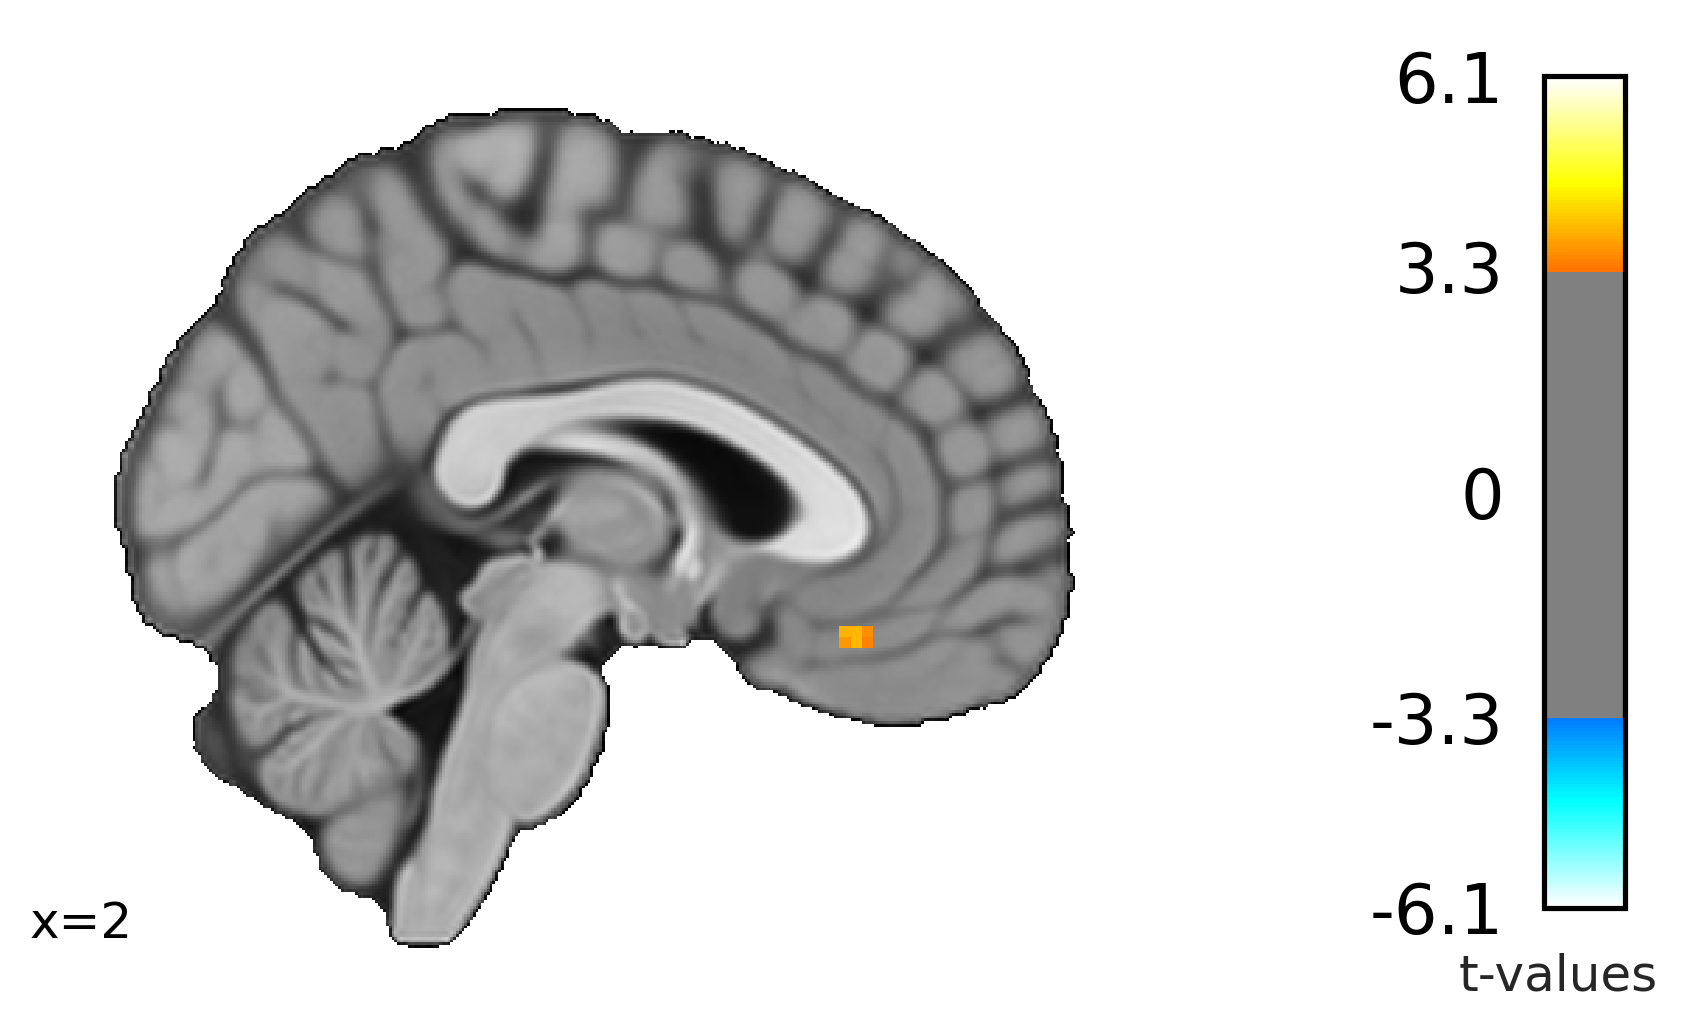
\includegraphics[width=\linewidth/2]{paper/src/figures/FigureS1_inaccessible_subsequent.png}
     \caption*{\textbf{Figure S1. Medial prefrontal cortex activation during guess responses given at the 24-hour category retrieval predicted the subsequent regain of conscious access to the memories.} \\ \vspace{0.5em}
     Medial prefrontal component of the episodic retrieval network predicted conscious recognition success. We contrasted the guess responses on the 24-hour category retrieval task that would subsequently yield correct sure responses on the recognition task with those other guess responses given on the 24-hour category task that would subsequently yield correct guess responses on the recognition task. This revealed a cluster in the medial prefrontal cortex (peak at MNI [0, 30, -16], p\textsubscript{uncor} < 0.001, T(18) = 4.19). Results presented in this panel were acquired with the whole-brain fMRI sequence. See Table S12 for details.}
\end{figure}

\newpage


 \begin{figure}[!ht]
    \centering
\begin{subfigure}[]{0.6\linewidth}
    \centering
    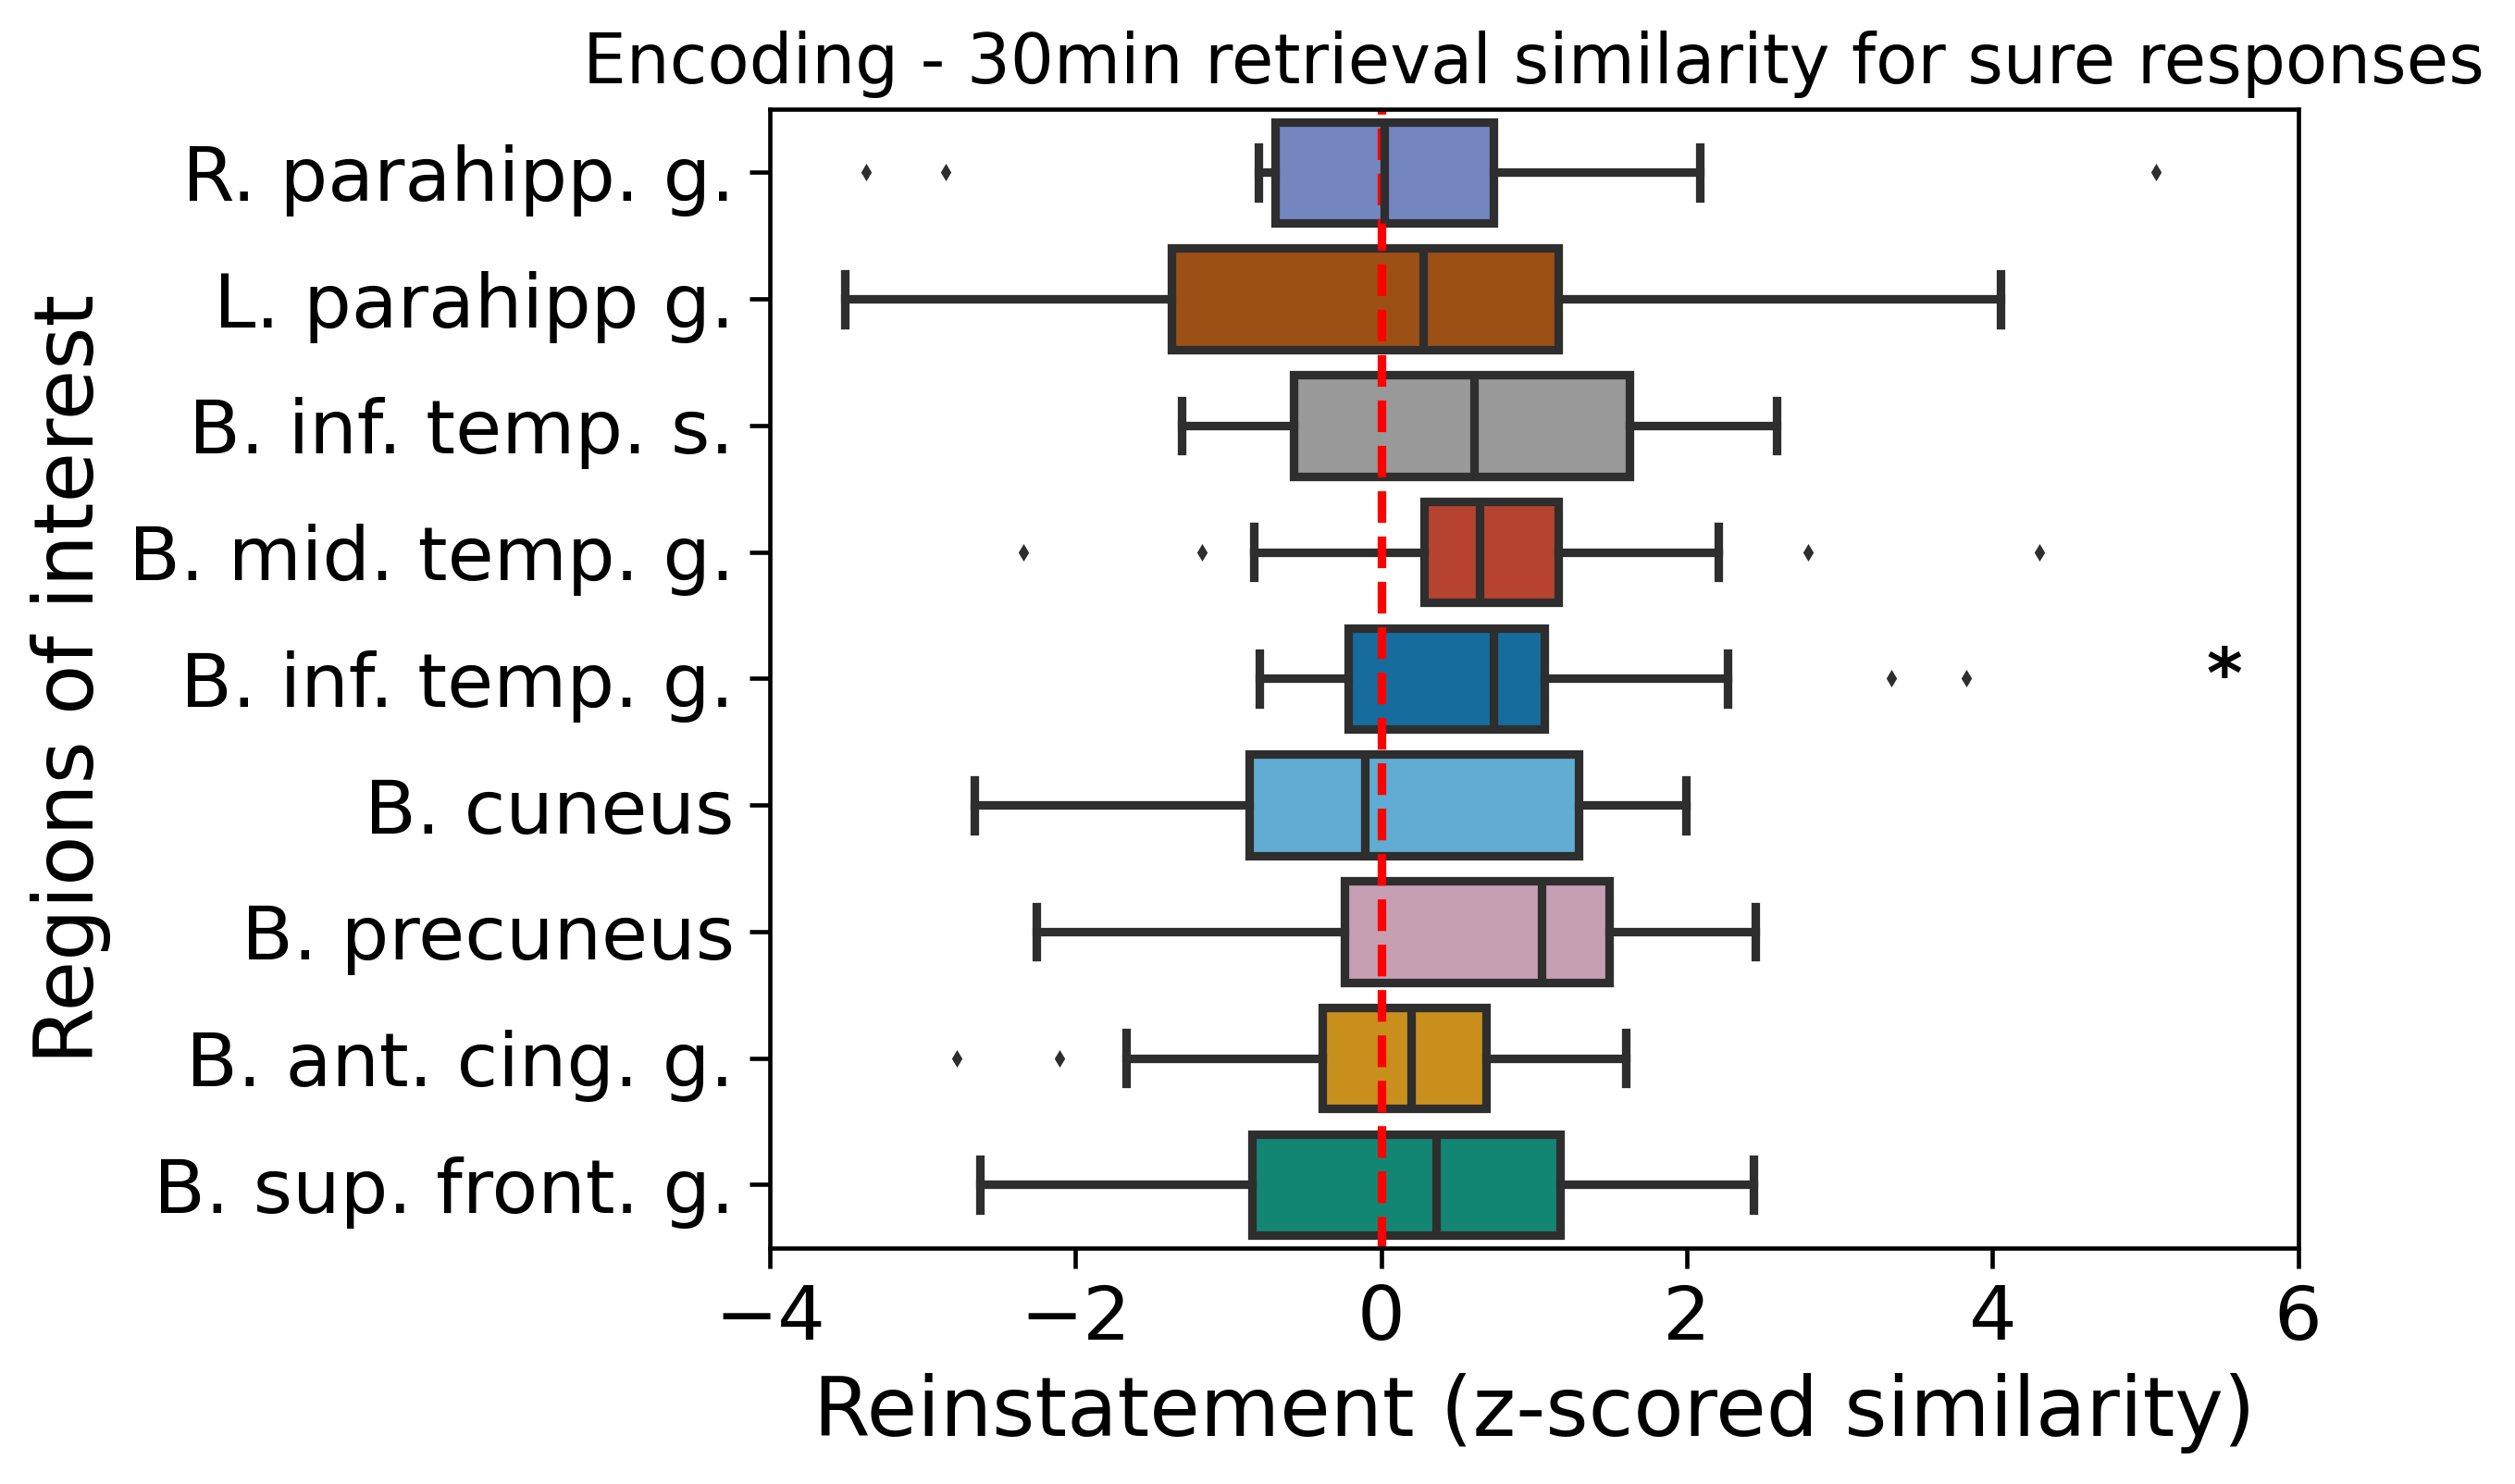
\includegraphics[width=\linewidth]{paper/src/figures/20240530_wb-array_n__enc_ret1_perm_consc_consc-unconsc_incorr.png}
\end{subfigure}
\begin{subfigure}[]{0.19\linewidth}
    \centering
    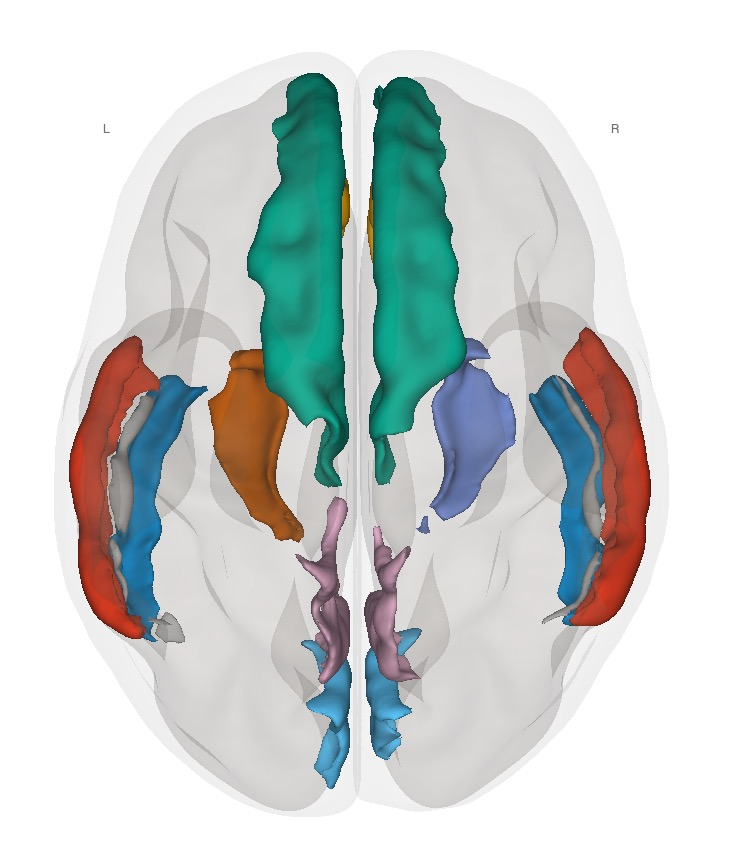
\includegraphics[width=\linewidth]{paper/src/figures/wb_rois_top.jpg}
\end{subfigure}
\begin{subfigure}[]{0.19\linewidth}
    \centering
    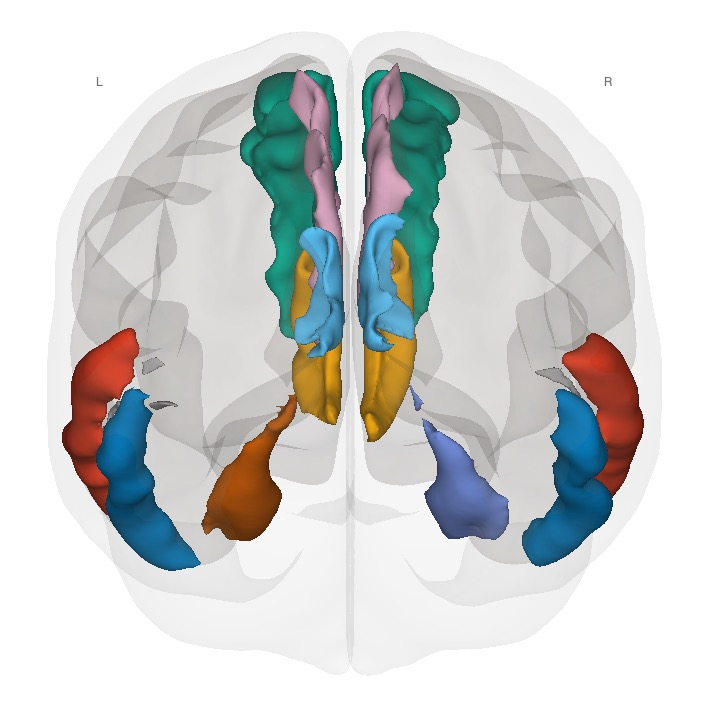
\includegraphics[width=\linewidth]{paper/src/figures/wb_rois_back.jpg}
\end{subfigure}
     \caption*{\textbf{Figure S2. Similarity of voxel patterns between encoding and the 30-minute category retrieval task were relevant for retrieval accuracy.} \\ \vspace{0.5em}
Encoding – retrieval similarity (ERS) analysis for the 30-minute category retrieval yielded significance in the bilateral inferior temporal gyrus for correct sure responses (t(16) = 2.3, p = 0.035, B\textsubscript{10} = 1.9).  Results presented in this panel were acquired with the whole-brain fMRI sequence. *p < 0.05, **p < 0.01 by Student’s t test. Abbreviations: R., right; L., left; B., bilateral; parahipp., parahippocampus; inf., inferior; mid., middle; ant., anterior; cing., cingulate; sup., superior; front., frontal; s., sulcus, g., gyrus.
}
\end{figure}

\newpage


 \begin{figure}[!ht]
    \centering
     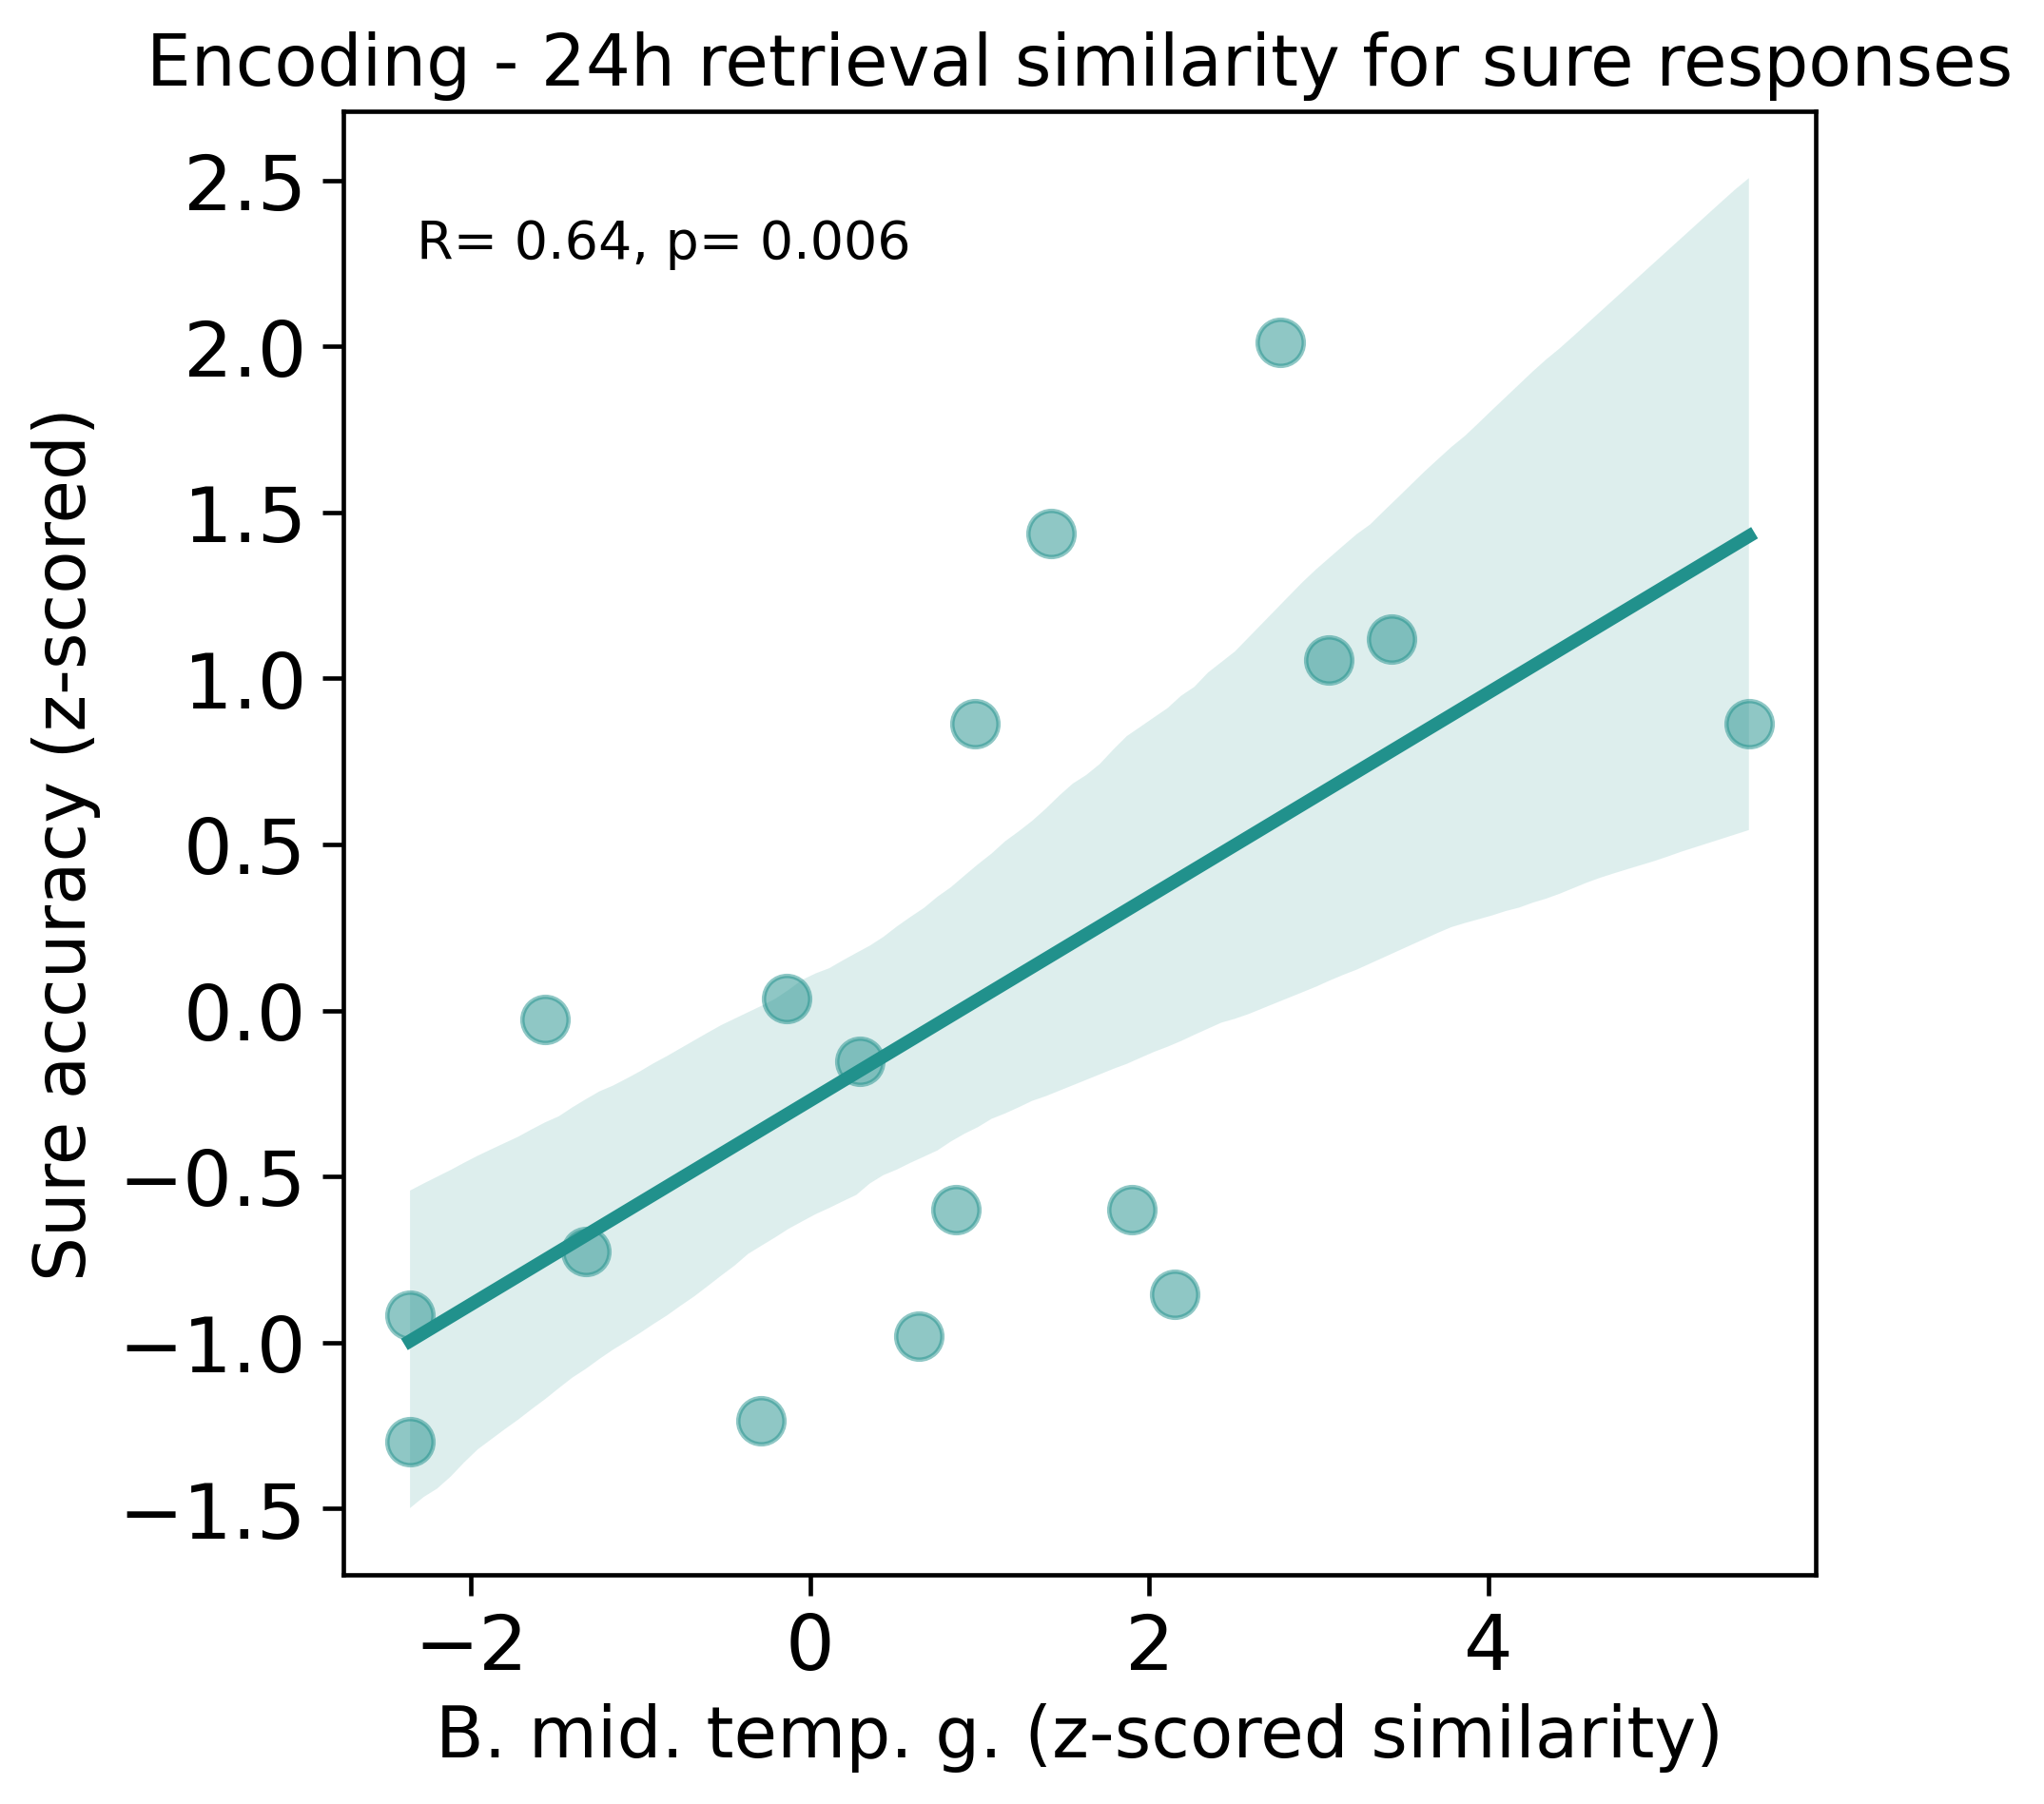
\includegraphics[width=0.6\linewidth]{paper/src/figures/20240530_wb-array_n__enc_ret2_perm_consc_consc-unconsc_incorr_B. mid. temp. g._ERS_correl.png}
     \caption*{\textbf{Figure S3. Similarity of voxel patterns between encoding and the 24-hour category retrieval were relevant for retrieval success.} \\ \vspace{0.5em}
   Encoding - 24-hour category retrieval similarity in bilateral middle temporal gyrus underlying correct sure responses given on the category retrieval task revealed a non-significant mean value comparison but a significant between-subjects correlation with the accuracy of sure responses given on the 24-hour category task (number of correct sure trials, p = 0.006, R = 0.64, B\textsubscript{10} = 10.4). Results presented in this panel were acquired with the whole-brain fMRI sequence. Abbreviations: B., bilateral; mid., middle; temp., temporal; g., gyrus.}
\end{figure}

\newpage

 \begin{figure}[!ht]
    \centering
     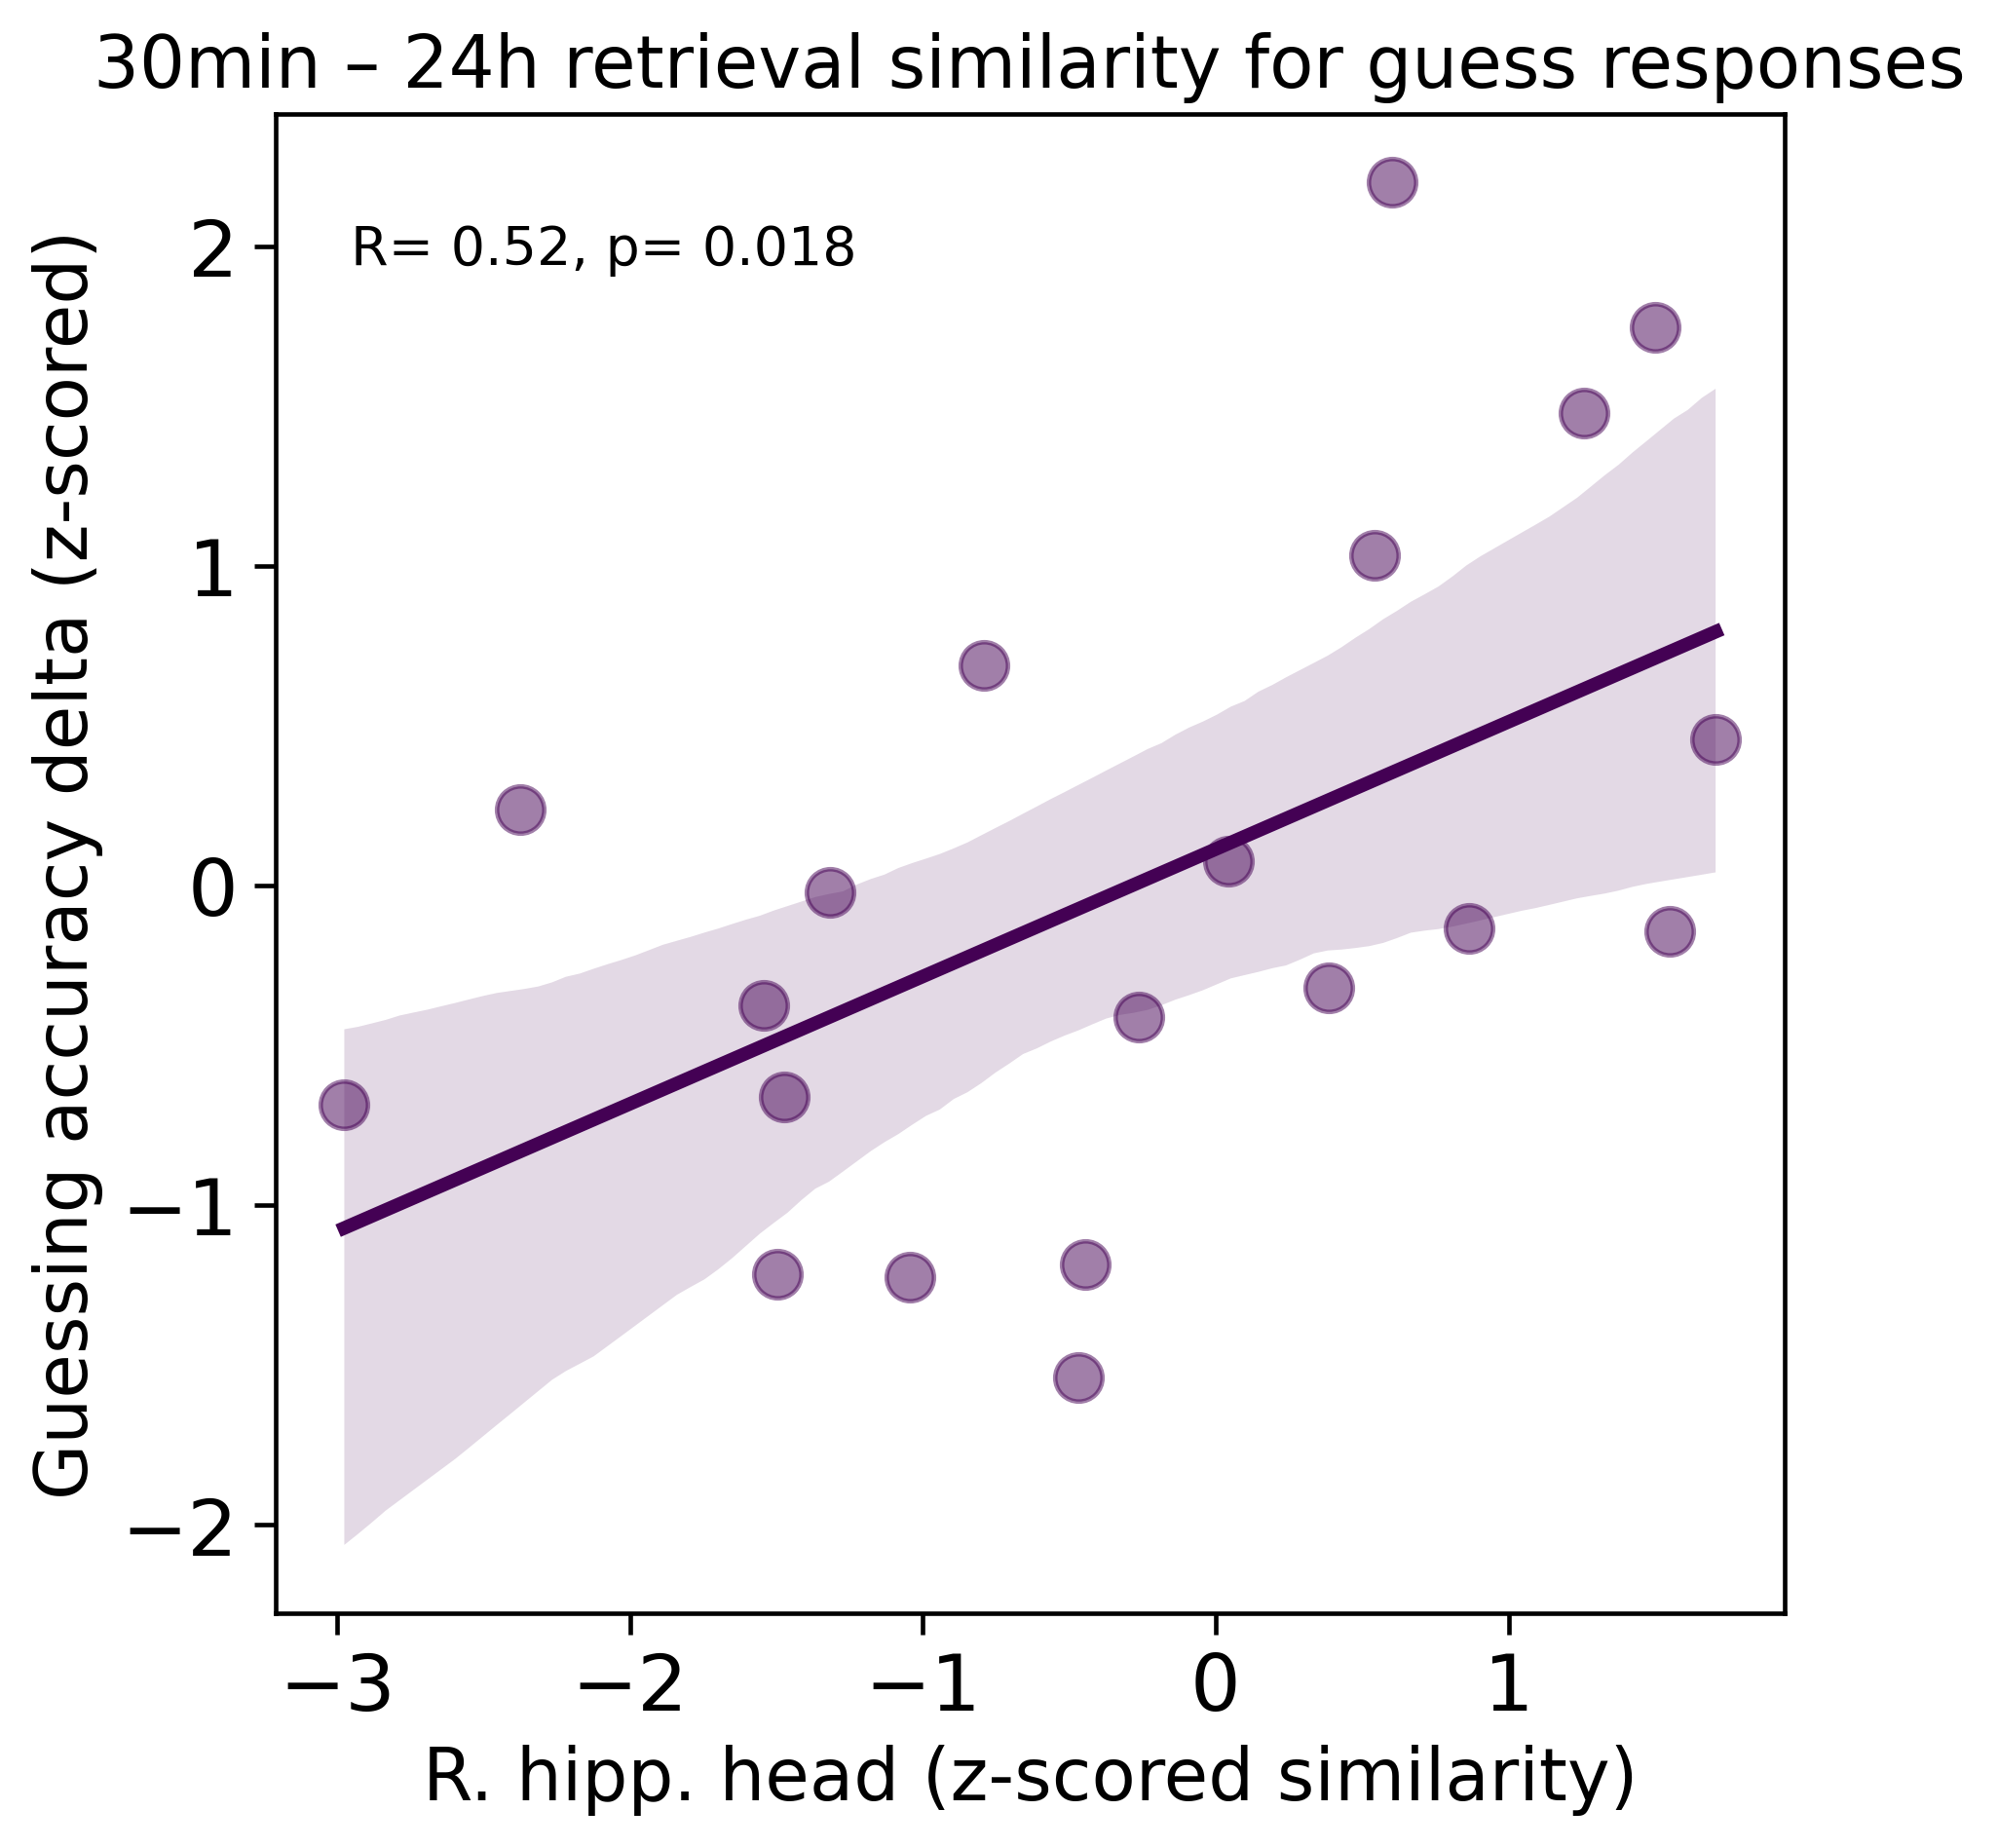
\includegraphics[width=\linewidth/2]{paper/src/figures/20240530_hipp-array_n_ret1_ret2_perm_consc_unconsc_corr-unconsc_incorr_R. hipp. head_ERS_correl.png}
     \caption*{\textbf{Figure S4. Similarity of voxel patterns between the 30-minute and the 24-hour category retrieval are relevant for the accuracy of guess responses.} \\ \vspace{0.5em}
Retrieval-retrieval similarity of voxel patterns in the right hippocampal head underlying correct guess responses revealed a non-significant mean value comparison but a significant between-subjects correlation with the delta of correct guess responses (i.e., number of correct guess responses at 24 hours minus number of correct guess responses at 30 minutes, p = 0.018, R = 0.52, B\textsubscript{10} = 3.7). Results presented in this panel were acquired with the small FOV fMRI sequence. Abbreviations: R., right; hipp., hippocampus.}
\end{figure}



\newpage

 \begin{figure}[!ht]
    \centering
\begin{subfigure}[]{0.6\linewidth}
    \centering
    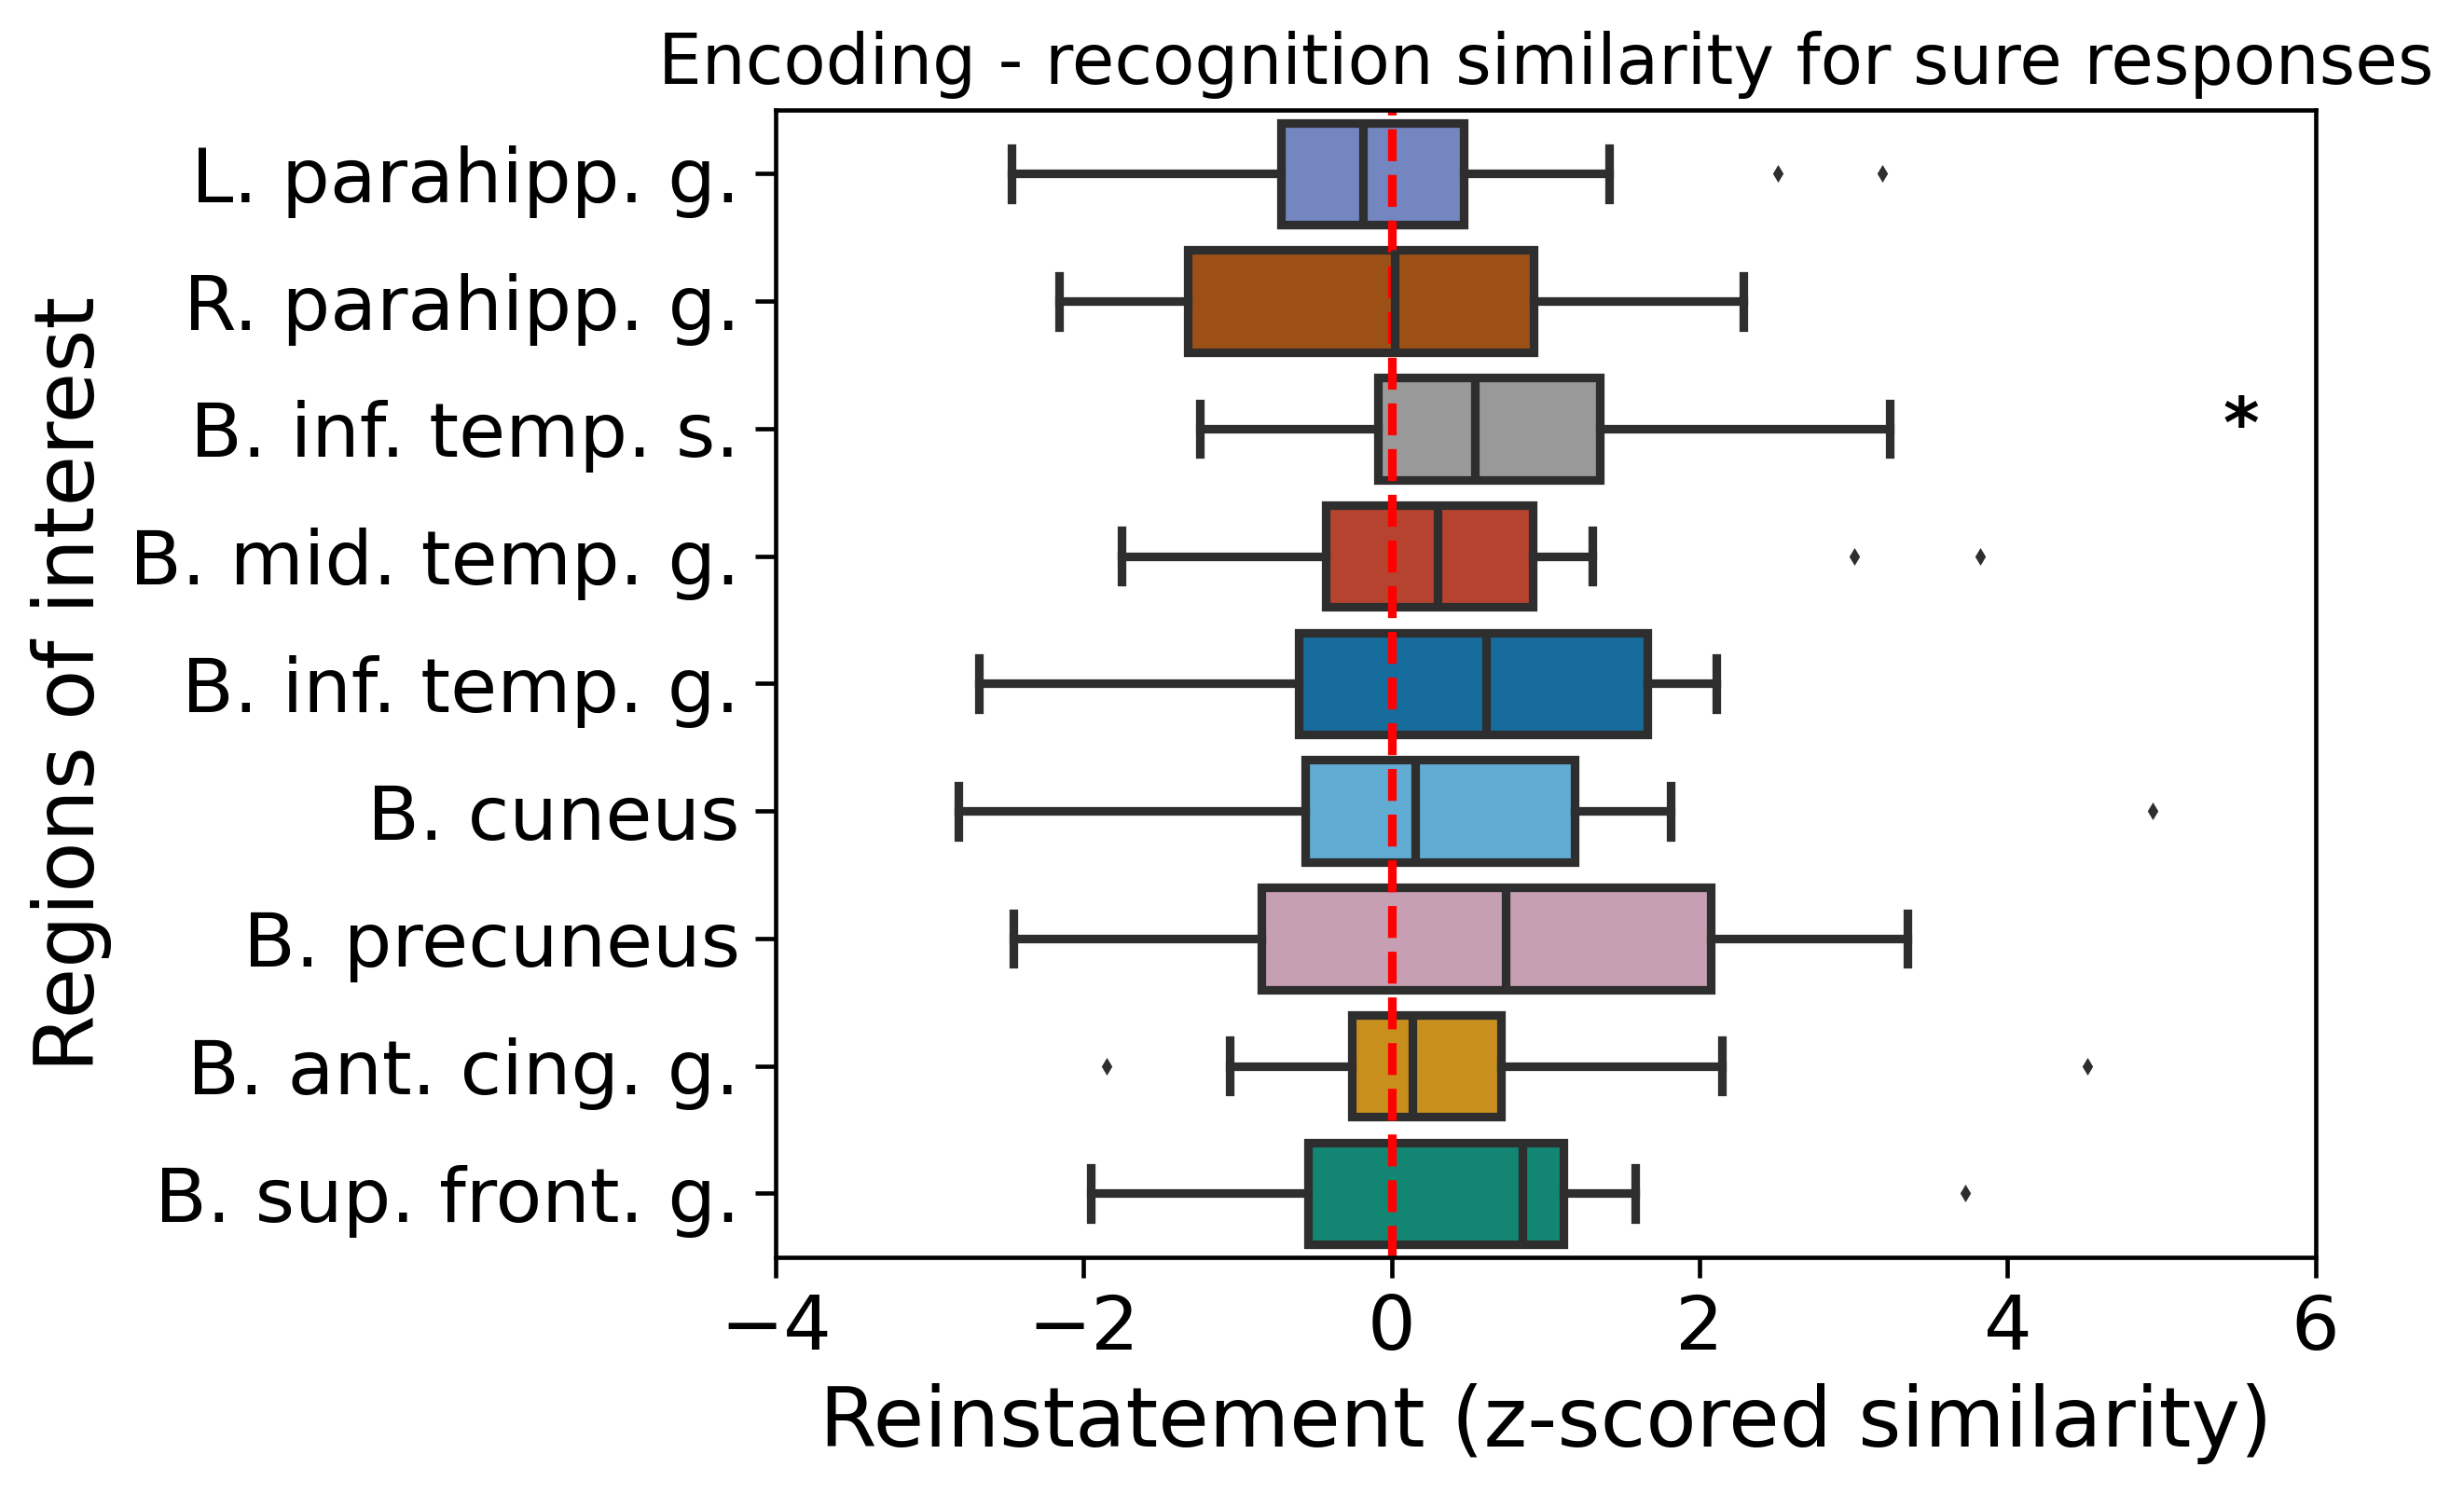
\includegraphics[width=\linewidth]{paper/src/figures/20240710_wb-all_memory_n_enc_recog_perm_consc_consc-unconsc_incorr.png}
\end{subfigure}
\begin{subfigure}[]{0.19\linewidth}
    \centering
    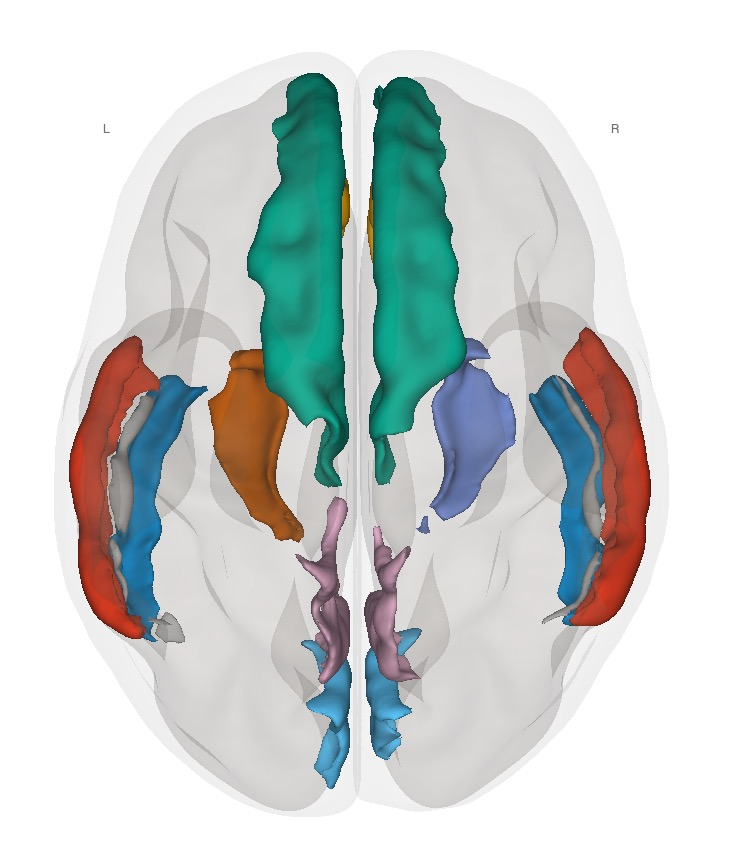
\includegraphics[width=\linewidth]{paper/src/figures/wb_rois_top.jpg}
\end{subfigure}
\begin{subfigure}[]{0.19\linewidth}
    \centering
    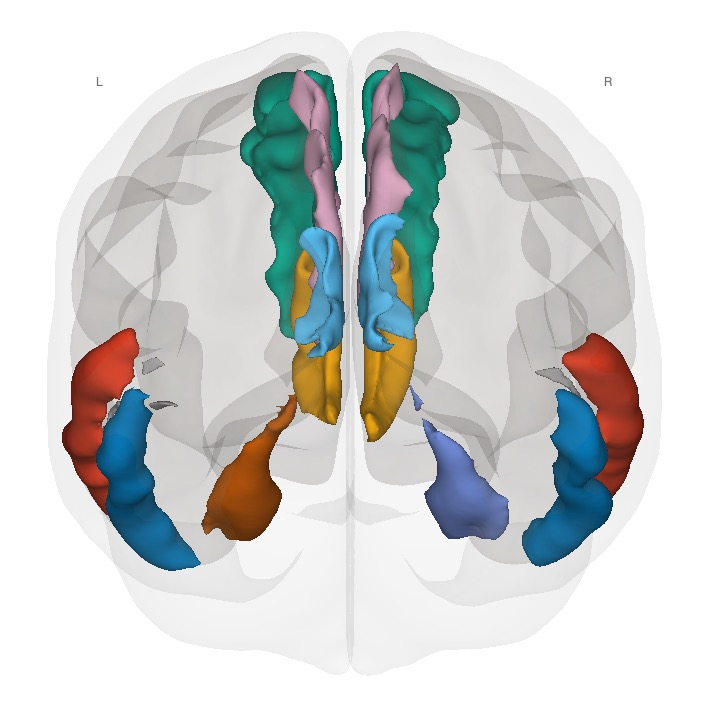
\includegraphics[width=\linewidth]{paper/src/figures/wb_rois_back.jpg}
\end{subfigure}
     \caption*{\textbf{Figure S5. Similarity of voxel patterns between encoding and recognition at 24 hours was relevant for retrieval success.} \\ \vspace{0.5em}
Significant mean value comparison in bilateral inferior temporal sulcus regarding correct sure responses (p = 0.026, t(17) = 2.55, B\textsubscript{10} = 2.9). Results presented in this panel were acquired with the whole-brain fMRI sequence. *p < 0.05, **p < 0.01 by Student’s t test. Abbreviations: R., right; L., left; B., bilateral; parahipp., parahippocampus; inf., inferior; mid., middle; ant., anterior; cing., cingulate; sup., superior; front., frontal; s., sulcus, g., gyrus.
}
\end{figure}


\newpage


 \begin{figure}[!ht]
    \centering
     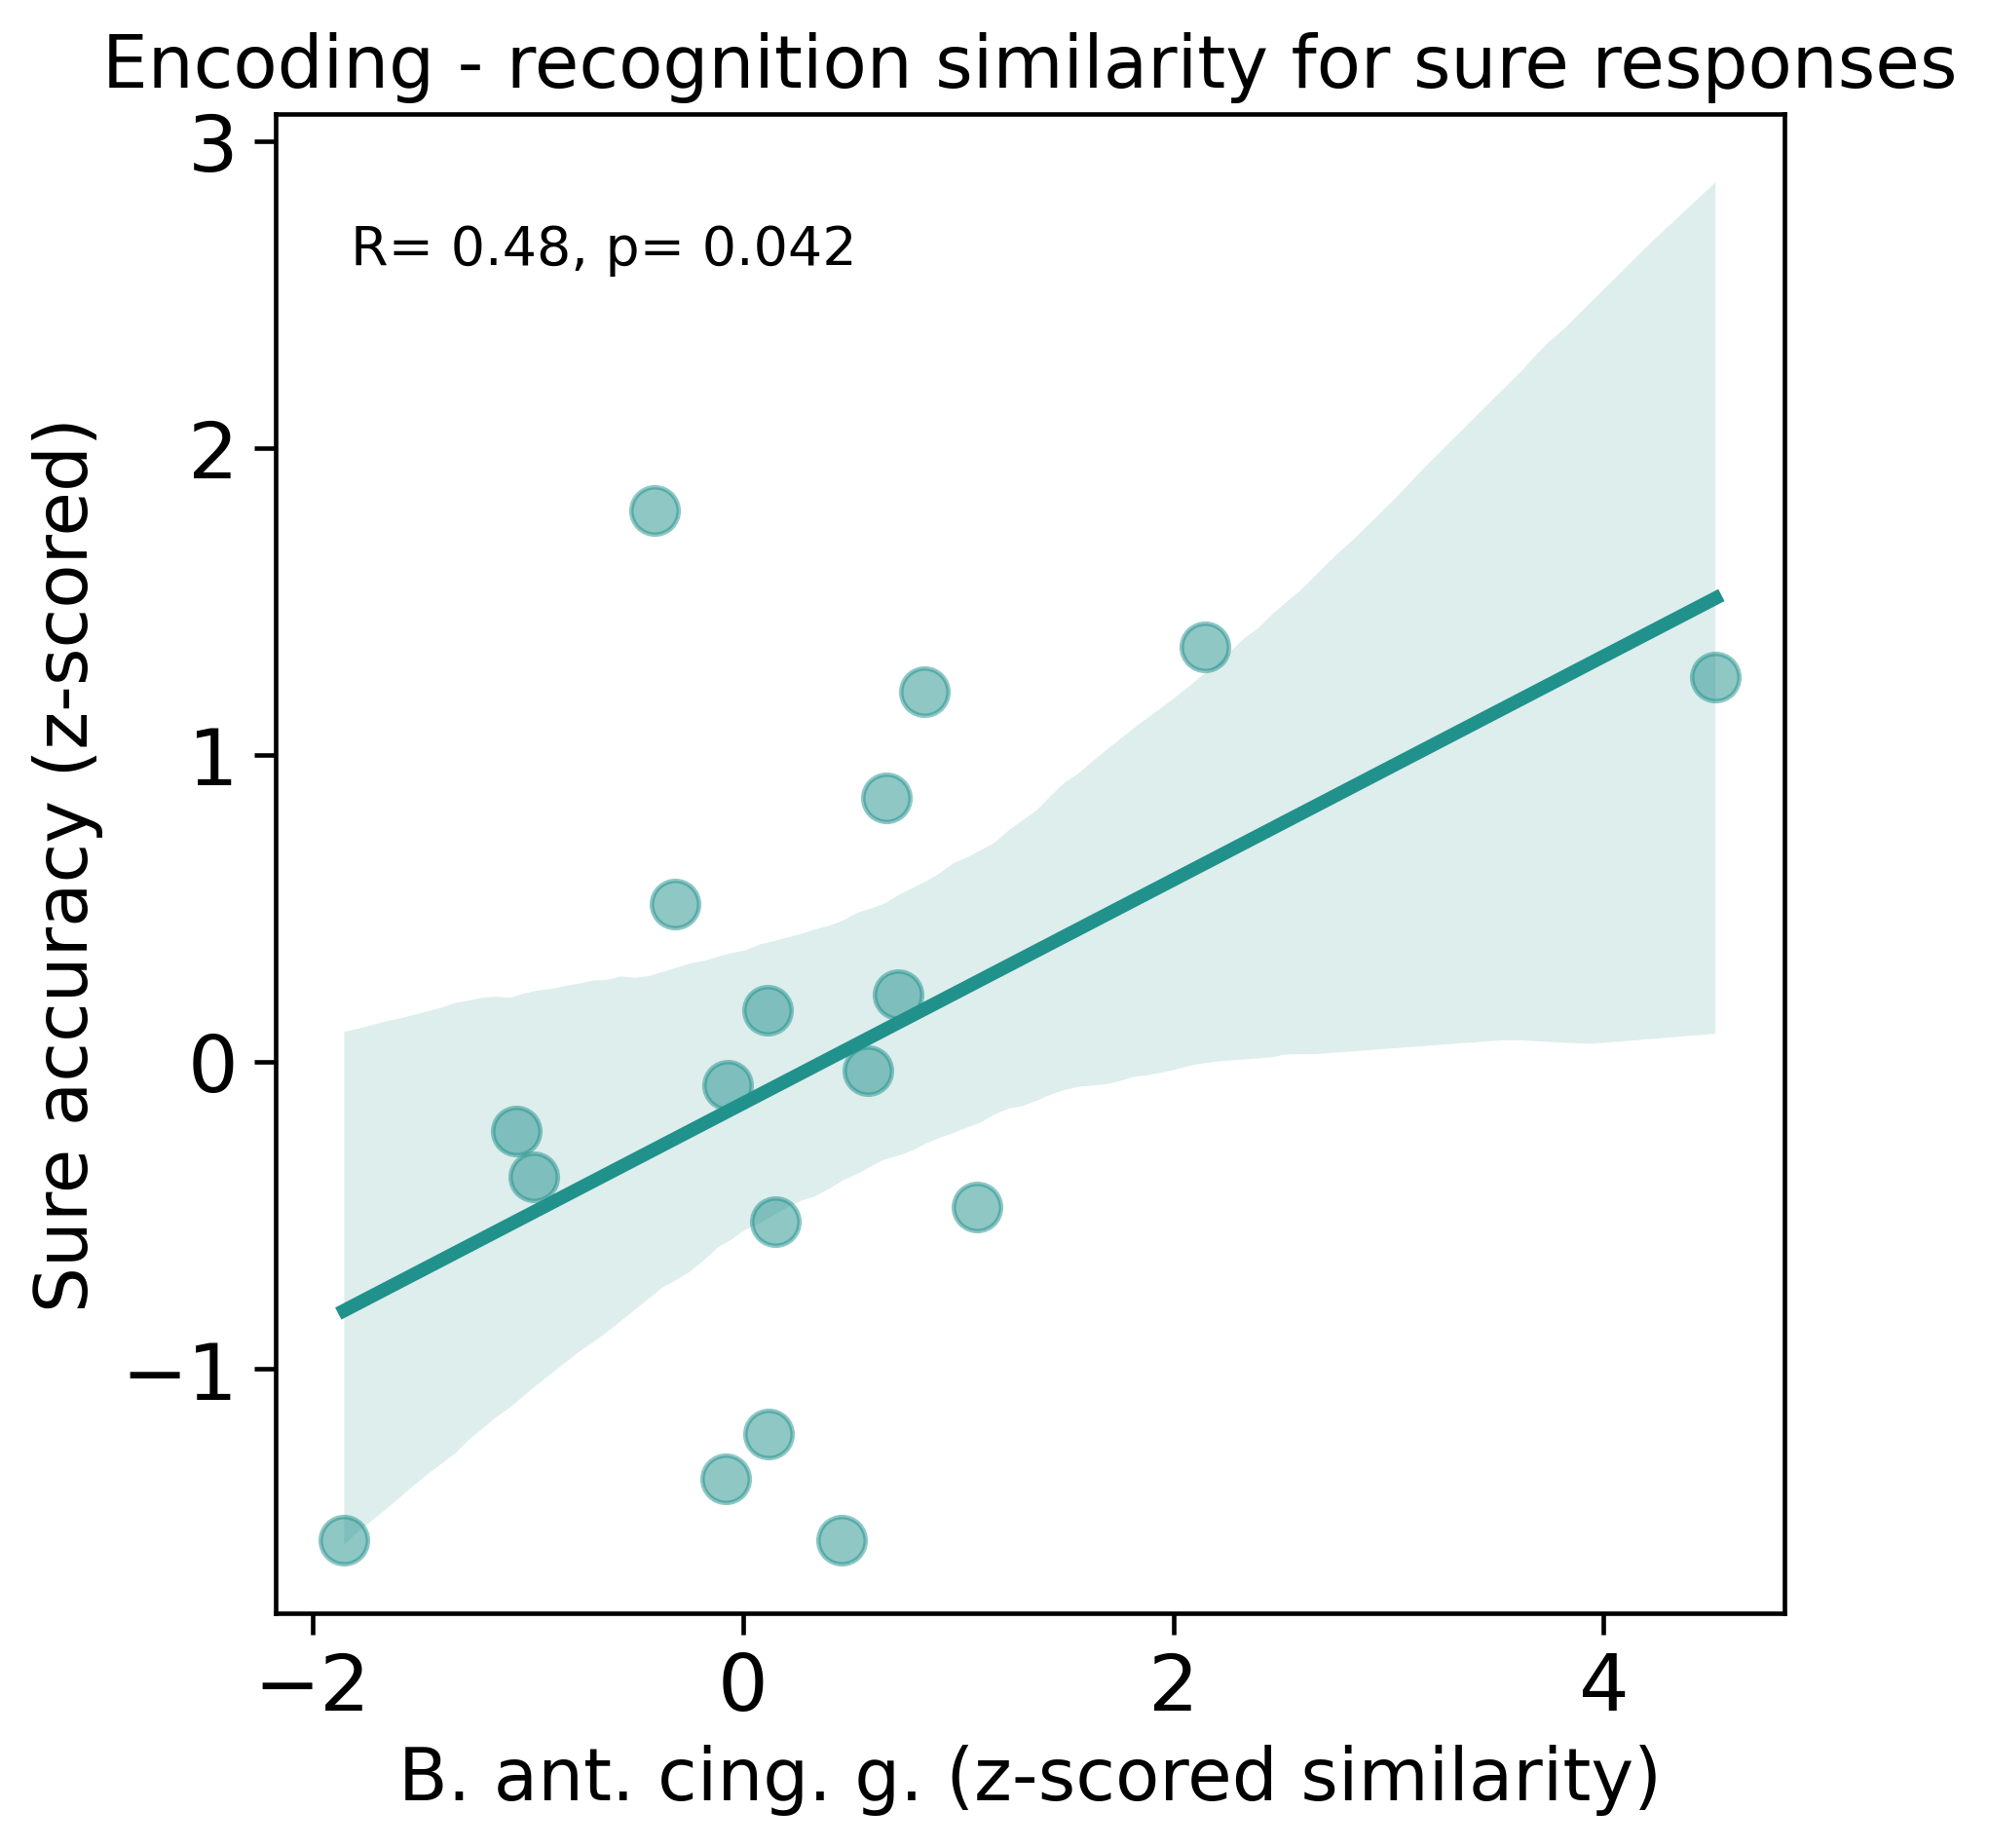
\includegraphics[width=\linewidth/2]{paper/src/figures/20240710_wb-all_memory_n_enc_recog_perm_consc_consc-unconsc_incorr_B. ant. cing. g._ERS_correl.png}
     \caption*{\textbf{Figure S6. Similarity of voxel patterns between encoding and recognition at 24 hours was relevant for retrieval success.} \\ \vspace{0.5em}
 Pattern similarity in bilateral anterior cingulate gyrus (B. ant. cing. g.) underlying correct sure responses revealed a non-significant mean value comparison but a significant between-subjects correlation with the number of correct sure responses given on the recognition task (p = 0.041, R = 0.48, B\textsubscript{10} = 2.0).  Results presented in this panel were acquired with the small FOV fMRI sequence. Abbreviations: B., bilateral; ant., anterior; cing., cingulate; g., gyrus.}
\end{figure}



%    \clearpage    
%    \input{paper/src/supplementary/appendix_tables.tex}
    
%\end{appendix}
%TC:endignore

\end{document}
